% created on 2019-12-13
% @author : bmazoyer
\documentclass[a4paper, twoside, openright]{book}
\usepackage[utf8]{inputenc}
\usepackage{helvet}
\renewcommand{\familydefault}{\sfdefault}
\usepackage{geometry}
\geometry{
left=22mm,
top=30mm,
right=22mm,
bottom=30mm
}
\usepackage{xcolor}
\definecolor{bordeau}{rgb}{0.3515625,0,0.234375}
\usepackage[absolute,overlay]{textpos}
\usepackage[]{graphicx}
\usepackage{lipsum}
\usepackage{array}
\usepackage{caption}
\usepackage{multicol}
\usepackage{hyperref}
\usepackage{afterpage}
\usepackage{setspace}
\usepackage{pgffor}
% Zach added packages--------||
\usepackage{comment}
\usepackage{amsmath,amssymb}
\usepackage{bm}
\usepackage{mathtools}
\usepackage{tikz}
\usepackage{color,soul}
\usepackage{fancyhdr}
\usepackage{tikz}
\usepackage{dirtree}
\usepackage{comment}
\excludecomment{zach}

\usepackage{pdfpages}

\usepackage[toc,page,header]{appendix}

% For CASToR algorithms -----------------------------------------------||
\usepackage[skins]{tcolorbox}
\usepackage[ruled]{algorithm2e} %vlined to gain room
% new comment style for algorithm package
\newcommand\mybluecomm[1]{\footnotesize\ttfamily\textcolor{blue}{#1}}
\SetCommentSty{mybluecomm}
%add a "step" keyword
\SetKw{KwStep}{step}
%------------------------------------------------------------------------||
% ToDo packages --------- -----------------------------------------------||
\usepackage[colorinlistoftodos,prependcaption,textsize=tiny]{todonotes}
\usepackage{xargs} 
\newcommandx{\unsure}[2][1=]{\todo[linecolor=red,backgroundcolor=red!25,bordercolor=red,#1]{#2}}
\newcommandx{\change}[2][1=]{\todo[linecolor=blue,backgroundcolor=blue!25,bordercolor=blue,#1]{#2}}
\newcommandx{\info}[2][1=]{\todo[linecolor=OliveGreen,backgroundcolor=OliveGreen!25,bordercolor=OliveGreen,#1]{#2}}
\newcommandx{\improvement}[2][1=]{\todo[linecolor=Plum,backgroundcolor=Plum!25,bordercolor=Plum,#1]{#2}}
\newcommandx{\thiswillnotshow}[2][1=]{\todo[disable,#1]{#2}}
%------------------------------------------------------------------------||


% Package for chapter summary in each chapter start
\usepackage{minitoc}


% Zach Commands 
\newcommand{\argmax}[1]{\underset{#1}{\operatorname{arg}\,\operatorname{max}}\;}

\def\bhline{\noalign{\ifnum0=`}\fi\hrule \@height  
\boldarrayrulewidth \futurelet \@tempa\@xhline}

\def\@xhline{\ifx\@tempa\hline\vskip \doublerulesep\fi
      \ifnum0=`{\fi}}
      
\newcommand{\br}{\ms\bhline\ms}
\newcommand{\mr}{\ms\hline\ms}

\DeclareMathSizes{10}{10}{7}{5}   % For size 10 text

\newcommand{\RNum}[1]{\uppercase\expandafter{\romannumeral #1\relax}}

% acronyms 
\usepackage[acronym, toc]{glossaries}
\glsdisablehyper 
\makeglossaries
%\thispagestyle{plain}
%\chaptermark{Abbreviation}
%\addcontentsline{toc}{chapter}{Abbreviations} \noindent
%\renewcommand{\nomname}{List of Abbreviations}

%--- Acronyms -----------------------------------------------------------------%
% \acrodef{label}[acronym]{written out form} % acronym syntax
%\acrodef{etacar}[$\eta$ Car]{Eta Carinae}   % acronym example
%--- Acronyms -----------------------------------------------------------------%
% how to use acronyms:
% \ac = use acronym, first time write both, full name and acronym
% \acf = use full name (text + acronym)
% \acs = only use acronym
% \acl = only use long text
% \acp, acfp, acsp, aclp = use plural form for acronym (append 's')
% \acsu, aclu = write + mark as used
% \acfi = write full name in italics and acronym in normal style
% \acused = mark acronym as used
% \acfip = full, emphasized, plural, used
%--- Acronyms -----------------------------------------------------------------%
%\chapter*{List of Abbreviations}
%\begin{acronym}
%        \acro{pet}[PET]{Positron Emission Tomography}
%\end{acronym}

\newacronym{pet}{PET}{Positron Emission Tomography}
\newacronym{spect}{SPECT}{Single-photon Emission Computed Tomography}
\newacronym{lor}{LOR}{Line of Response}
\newacronym{fdg}{FDG}{Fluorodeoxyglucose}
\newacronym{hybrid}{HYBRID}{Healthcare Yearns for Bright Researchers for Imaging Data}
\newacronym{itn}{ITN}{Initial Training Network}
\newacronym{pmt}{PMT}{Photomultiplier Tube}
\newacronym{sipm}{SiPM}{Silicon Photomultiplier}
\newacronym{fov}{FOV}{Field of View}
\newacronym{ct}{CT}{Computed Tomography}
\newacronym{mr}{MR}{Magnetic Resonance }
\newacronym{fbp}{FBP}{Filtered Back Projection}
\newacronym{castor}{CASToR}{Customizable and Advanced Software for Tomographic Reconstruction}
\newacronym{psf}{PSF}{Point Spread Function}
\newacronym{sop}{SOP}{Standard Operating Procedure}
\newacronym{nsclc}{NSCLC}{Non-Small-Cell Lung Carcinoma}
\newacronym{mip}{MIP}{Maximum Intensity Projection}
\newacronym{tof}{TOF}{Time of Flight}
\newacronym{tac}{TAC}{Time Activity Curve}
\newacronym{nhp}{NHP}{Non-Human Primate}

% nomenclature:
\newglossaryentry{angelsperarea}{
  name = $a$ ,
  description = The number of angels per unit area,
}
\newglossaryentry{numofangels}{
  name = $N$ ,
  description = The number of angels per needle point
}
\newglossaryentry{areaofneedle}{
  name = $A$ ,
  description = The area of the needle point
}



% No new paragraphs indentation 
\usepackage[parfill]{parskip}

% Add some colours for highlighting 
\usepackage{color,soul}

%SI units 
\usepackage{siunitx}

% Rules for tables with extra space around
\usepackage{booktabs }

% Chemistry and isotopes
\usepackage[version=4]{mhchem}

% Greek !!
\usepackage[greek,english]{babel}
\usepackage{alphabeta}
%----------------------------||
\setlength{\columnseprule}{0pt}
\setlength\columnsep{10pt}

\newcommand\blankpage{%
    \null
    \thispagestyle{empty}%
    \addtocounter{page}{-1}%
    \newpage}

%Bibliography style
\usepackage[sort&compress, square, numbers]{natbib}
%\bibliographystyle{abbrvnat}
\bibliographystyle{unsrtnat}
%\usepackage{notoccite}

% Thesis title
\newcommand{\PhDTitle}{Modelling and Reconstruction of \mbox{Whole Body} parametric maps in PET-MRI Pharmacological imaging} 

% Name
\newcommand{\PhDname}{Zacharias Chalampalakis} 

% PDF metadata
\hypersetup{
	pdfauthor={\PhDname},
	pdfsubject={Manuscrit de thèse de doctorat},
	pdftitle={\PhDTitle}
}

% Zach added configuration --------------------------------------------------

% Place title on top of each page and page numbers
\pagestyle{fancy}
\fancyhf{}
\fancyhead[ER]{\nouppercase\leftmark}
%\fancyhead[ER]{\if@mainmatter \nouppercase\leftmark\fi}
\fancyhead[OL]{\nouppercase\rightmark}
\fancyhead[EL,OR]{\thepage}


\begin{document}
	\doublespacing
	
    %%%%%%%%%%%%%%%%%%%%%%%%%%%%%%%%%%%%%%%%%%%%%%%%%%%%%%%%%%%%%%%%%%%%%%%%%%%%%%%%%%%%%%%%%%%%%%%%%%%%%%%%%%%%%%%%%%%%%%%%%%%%%%%%%%%%%%%%%%%%%%%%%%%%%%%%%%%%%%%%%%%%%%%
%%%%%%%%%%%%%%%%%%%%%%%%%%%%%%%%%%%%%%%%%%%%%%%%%%%%%%%%%%%%%%%%%%%%%%%%%%%%%%%%%%%%%%%%%%%%%%%%%%%%%%%%%%%%%%%%%%%%%%%%%%%%%%%%%%%%%%%%%%%%%%%%%%%%%%%%%%%%%%%%%%%%%%%
%%% Modèle pour la 1ère de couverture des thèses préparées à l'Université Paris-Saclay, basé sur le modèle produit par Guillaume BRIGOT / Template for back cover of thesis made at Université Paris-Saclay, based on the template made by Guillaume BRIGOT
%%% Mis à jour par Aurélien ARNOUX (École polytechnique)/ Updated by Aurélien ARNOUX (École polytechnique)
%%% Les instructions concernant chaque donnée à remplir sont données en bloc de commentaire / Rules to fill this file are given in comment blocks
%%% ATTENTION Ces informations doivent tenir sur une seule page une fois compilées / WARNING These informations must contain in no more than one page once compiled
%%%%%%%%%%%%%%%%%%%%%%%%%%%%%%%%%%%%%%%%%%%%%%%%%%%%%%%%%%%%%%%%%%%%%%%%%%%%%%%%%%%%%%%%%%%%%%%%%%%%%%%%%%%%%%%%%%%%%%%%%%%%%%%%%%%%%%%%%%%%%%%%%%%%%%%%%%%%%%%%%%%%%%%
%%% Version du 23 mai 2019 (Merci à Thibault CHEVALÉRIAS (CEA) pour ses suggestions et corrections)
%%%%%%%%%%%%%%%%%%%%%%%%%%%%%%%%%%%%%%%%%%%%%%%%%%%%%%%%%%%%%%%%%%%%%%%%%%%%%%%%%%%%%%%%%%%%%%%%%%%%%%%%%%%%%%%%%%%%%%%%%%%%%%%%%%%%%%%%%%%%%%%%%%%%%%%%%%%%%%%%%%%%%%%


\label{form_first}

%%% Formulaire / Form
%%% Remplacer les paramètres des \newcommand par les informations demandées / Replace \newcommand parameters by asked informations
%%%


\newcommand{\NNT}{20XXSACLXXXX} 															%% Numéro National de Thèse (donnée par la bibliothèque à la suite du 1er dépôt)/ National Thesis Number (given by the Library after the first deposit)

\newcommand{\ecodoctitle}{Dénomination} 													%% Nom de l'ED. Voir site de l'Université Paris-Saclay / Full name of Doctoral School. See Université Paris-Saclay website
\newcommand{\ecodocacro}{Sigle}																%% Sigle de l'ED. Voir site de l'Université Paris-Saclay / Acronym of the Doctoral School. See Université Paris-Saclay website
\newcommand{\ecodocnum}{000} 																%% Numéro de l'école doctorale / Doctoral School number
\newcommand{\PhDspeciality}{voir spécialités par l'ED} 										%% Spécialité de doctorat / Speciality 
\newcommand{\PhDworkingplace}{Nom de l'établissement} 										%% Établissement de préparation / PhD working place : l'Université Paris-Sud, l'Université de Versailles-Saint-Quentin-en-Yvelines, l'Université d'Evry-Val-d'Essonne, l'Institut des sciences et industries du vivant et de l'environnement (AgroParisTech), CentraleSupélec,l'Ecole normale supérieure de Cachan, l'Ecole Polytechnique, l'Ecole nationale supérieure de techniques avancées, l'Ecole nationale de la statistique et de l’administration économique, HEC Paris, l'Institut d'optique théorique et appliquée, Télécom ParisTech, Télécom SudParis   
\newcommand{\defenseplace}{Ville de soutenance} 											%% Ville de soutenance / Place of defense
\newcommand{\defensedate}{Date} 															%% Date de soutenance / Date of defense

%%% Établissement / Institution
%%% Si la thèse a été produite dans le cadre d'une co-tutelle, commenter la partie "Pas de co-tutelle" et décommenter la partie "Co-tutelle" / If the thesis has been prepared in guardianship, comment the part "Pas de co-tutelle" and uncomment the part "Co-tutelle"

	%%%%%%%%%%%%%%%%%%%%%%%%%
	%%% Pas de co-tutelle %%%
	%%%%%%%%%%%%%%%%%%%%%%%%%

\newcommand{\logoEtt}{blank}																%% NE PAS MODIFIER / DO NOT MODIFY
\newcommand{\vpostt}{0.1} 																	%% NE PAS MODIFIER / DO NOT MODIFY
\newcommand{\hpostt}{6}																		%% NE PAS MODIFIER / DO NOT MODIFY
\newcommand{\logoEt}{etab} 																	%% Logo de l'établissement de soutenance. Indiquer le sigle / Institution logo. Indicate the acronym : AGRO, CENTSUP, ENS, ENSAE, ENSTA, HEC, IOGS, TPT, TSP, UEVE, UPSUD, UVSQ, X 
\newcommand{\vpos}{0.1}																		%% À modifier au besoin pour aligner le logo verticalement / If needed, modify to align logo vertilcally
\newcommand{\hpos}{11}																		%% À modifier au besoin pour aligner le logo horizontalement / If needed, modify to align logo horizontaly

		%%%%%%%%%%%%%%%%%%
		%%% Co-tutelle %%%
		%%%%%%%%%%%%%%%%%%

%\newcommand{\logoEt}{etab} 																%% Logo de l'université partenaire. Placer le fichier .png dans le répertoire '/media/etab' et indiquer le nom du fichier sans l'extension / Logo of partner university. Place the .png file in the directory '/media/etab' and point the file name without the extension
%\newcommand{\vpos}{0.1}																	%% À modifier au besoin pour aligner les logos verticalement / If needed, modify to align logos vertilcally
%\newcommand{\hpos}{11}																		%% À modifier au besoin pour aligner les logos horizontalement / If needed, modify to align logos horizontaly
%\newcommand{\logoEtt}{etab2}  																%% Logo de l'établissement de soutenance. Le nom du fichier correspond au sigle de l'établissement /  Institution logo. Filename correspond to institution acronym : AGRO, CENTSUP, ENS, ENSAE, ENSTA, HEC, IOGS, TPT, TSP, UEVE, UPSUD, UVSQ, X 
%\newcommand{\vpostt}{0.1} 																	%% À modifier au besoin pour aligner les logos verticalement / If needed, modify to align logos vertilcally
%\newcommand{\hpostt}{6}																	%% À modifier au besoin pour aligner les logos horizontalement / If needed, modify to align logos horizontaly


%%% JURY

% Lors du premier dépôt de la thèse le nom du président n’est pas connu, le choix du président se fait par les membres du Jury juste avant la soutenance. La précision est apportée sur la couverture lors du second dépôt / Choice of the jury's president is made during the defense. Thus, it must be specified only for the second file deposition in ADUM.
% Tous les membres du juty listés doivent avoir été présents lors de la soutenance / All the jury members listed here must have been present during the defense.

%%% Membre n°1 (Président) / Member n°1 (President)
\newcommand{\jurynameA}{Prénom Nom}
\newcommand{\juryadressA}{Statut, Établissement (Unité de recherche)}
\newcommand{\juryroleA}{Président}

%%% Membre n°2 (Rapporteur) / Member n°2 (Reviewer)
\newcommand{\jurynameB}{Prénom Nom}
\newcommand{\juryadressB}{Statut, Établissement (Unité de recherche)}
\newcommand{\juryroleB}{Rapporteur}

%%% Membre n°3 (Rapporteur) / Member n°3 (Reviewer)
\newcommand{\jurynameC}{Prénom Nom}
\newcommand{\juryadressC}{Statut, Établissement (Unité de recherche)}
\newcommand{\juryroleC}{Rapporteur}

%%% Membre n°4 (Examinateur) / Member n°4 (Examiner)
\newcommand{\jurynameD}{Prénom Nom}
\newcommand{\juryadressD}{Statut, Établissement (Unité de recherche)}
\newcommand{\juryroleD}{Examinateur}

%%% Membre n°5 (Directeur de thèse) / Member n°5 (Thesis supervisor)
\newcommand{\jurynameE}{Claude COMTAT}
\newcommand{\juryadressE}{Professeur, Université Paris-Saclay, CEA, CNRS, Inserm (Laboratoire d’Imagerie Biomédicale Multimodale Paris Saclay)}
\newcommand{\juryroleE}{Directeur de thèse}

%%% Membre n°6 (Co-directeur de thèse) / Member n°6 (Thesis co-supervisor)
\newcommand{\jurynameF}{Prénom Nom}
\newcommand{\juryadressF}{Statut, Établissement (Unité de recherche)}
\newcommand{\juryroleF}{Co-directeur de thèse}

%%% Membre n°7 (Invité) / Member n°7 (Guest)
\newcommand{\jurynameG}{Prénom Nom}
\newcommand{\juryadressG}{Statut, Établissement (Unité de recherche)}
\newcommand{\juryroleG}{Invité}

%%% Membre n°8 (Invité) / Member n°8 (Guest)
\newcommand{\jurynameH}{Prénom Nom}
\newcommand{\juryadressH}{Statut, Établissement (Unité de recherche)}
\newcommand{\juryroleH}{Invité}

%% Il est possible d'ajouter des membres supplémentaires selon le même modèle / More jury members can be added according to the same model

\label{layout_first}
%%% Mise en page / Page layout      
%%% NE RIEN MODIFIER EXCEPTÉ LA PARTIE CONCERNANT LE JURY (voir \label{jury}) SI BESOIN / DO NOT MODIFY EXCEPT SECTION CONCERNING JURY (see \label{jury}) IF NEEDED
%%%%%%%%%%%%%%%%%%%%%%%%%%%%%%%%%%%%%%%%%%%%%%%%%%%%%%%%%%%%%%%%%%%%%%%%%%%%%%%%%%%%%%%%%%%%%%%%%%%%%%%%%%%%%%%%%%%%%%%%%%%%%%%%%%%%%%%%%%%%%%%%%%%%%%%%%%%%%%%%%%%%%%%
%%%%%%%%%%%%%%%%%%%%%%%%%%%%%%%%%%%%%%%%%%%%%%%%%%%%%%%%%%%%%%%%%%%%%%%%%%%%%%%%%%%%%%%%%%%%%%%%%%%%%%%%%%%%%%%%%%%%%%%%%%%%%%%%%%%%%%%%%%%%%%%%%%%%%%%%%%%%%%%%%%%%%%%




\thispagestyle{empty}
.
\begin{textblock}{5}(0,0)
	\textblockcolour{bordeau}
	
\includegraphics [scale=1]{media/bande.png}
	\vspace{300mm}
\end{textblock}

\begin{textblock}{1}(0.6,9.5)
	
	\Huge{\rotatebox{90}{\color{white}{\fontsize{38}{54}\selectfont Thèse de doctorat}}}
\end{textblock}

\begin{textblock}{1}(0.6,3)
	\Large{\rotatebox{90}{\color{white}{NNT : \NNT}}}
\end{textblock}

\begin{textblock}{1}(\hpostt,\vpostt)
	\textblockcolour{white}
	
\includegraphics[scale=1]{media/ed/EOBE.jpeg}
\end{textblock}

%\begin{textblock}{1}(\hpos,\vpos)
%	\textblockcolour{white}
%		\includegraphics[scale=1]{media/etab/\ilogo}	
%\end{textblock}


%% Texte
\begin{singlespace}
\begin{textblock}{10}(5.7,3)
	\textblockcolour{white}
	
	\color{bordeau}
	\begin{flushright}

		\huge{\PhDTitle} \bigskip %% Titre de la thèse 
		\vfill
		\color{black} %% Couleur noire du reste du texte
		\normalsize {Thèse de doctorat de l'Université Paris-Saclay} \\
		préparée à \PhDworkingplace \\ \bigskip
		\vfill
		École doctorale n$^{\circ}$\ecodocnum ~\ecodoctitle ~(\ecodocacro)  \\
		
		\small{Spécialité de doctorat: \PhDspeciality} \bigskip %% Spécialité 
		\vfill  
		\footnotesize{Thèse présentée et soutenue à \defenseplace, le \defensedate, par} \bigskip
		\vfill
		\Large{\textbf{\textsc{\PhDname}}} %% Nom du docteur
		\vfill
	\end{flushright}
	
	\color{black}
	%% Jury
	\begin{flushleft}
		
		\small Composition du Jury :
	\end{flushleft}
	%% Members of the jury

	\small
	%\begin{center}
	\newcolumntype{L}[1]{>{\raggedright\let\newline\\\arraybackslash\hspace{0pt}}m{#1}}
	\newcolumntype{R}[1]{>{\raggedleft\let\newline\\\arraybackslash\hspace{0pt}}lm{#1}}
	
	\label{jury} 																				%% Mettre à jour si des membres ont été ajoutés ou retirés / Update if members have been added or removed
	\begin{flushleft}
	\begin{tabular}{@{} L{9.5cm} R{4.5cm}}
		\jurynameA  \\ \juryadressA & \juryroleA \\[5pt]
		\jurynameB  \\ \juryadressB & \juryroleB \\[5pt]
		\jurynameC  \\ \juryadressC & \juryroleC \\[5pt]
		\jurynameD  \\ \juryadressD & \juryroleD \\[5pt]
		\jurynameE  \\ \juryadressE & \juryroleE \\[5pt]
		\jurynameF  \\ \juryadressF & \juryroleF \\[5pt]
		\jurynameG  \\ \juryadressG & \juryroleG \\[5pt]
		\jurynameH  \\ \juryadressH & \juryroleH \\[5pt]
	\end{tabular} 
	\end{flushleft}   
	%\end{center}
\end{textblock}
\end{singlespace}
\afterpage{\blankpage}
    
    % created on 2019-12-13
% @author : bmazoyer
\newenvironment{dedication}
  {\clearpage           % we want a new page
   \thispagestyle{empty}% no header and footer
   \vspace*{\stretch{1}}% some space at the top 
   \itshape             % the text is in italics
   \raggedleft          % flush to the right margin
  }
  {\par % end the paragraph
   \vspace{\stretch{3}} % space at bottom is three times that at the top
   \clearpage           % finish off the page
  }
  
\begin{dedication}
Dedication
\end{dedication}
\afterpage{\blankpage}
    \cleardoublepage
    
    % created on 2019-12-13
% @author : bmazoyer
\chapter*{Acknowledgements}

First and foremost, I want to thank my primary supervisor Dr Claude Comtat who believed in me and supported me every step of the way during my PhD project. I thank him for the patience he showed while discussing all my questions and ideas and his experience in guiding me throughout this project. Without ever applying pressure on me he has inspired me to deepen my knowledge and solidify my understanding of all involved concepts in our project.
 After these years working together, beyond the scientific values that he passed to me I have learned a lot about patience and being humble.

In addition, I want to thank my second supervisor Dr Simon Stute who provided me with the tools and technical knowledge to kick-off my project and also for sharing his vision of the CASToR tools with me and his more practical point of view of the research in the field.
With that, I want to also thank the CASToR collaboration and development team, particularly Dr Simon Stute, Dr Thibaut Merlin and Dr Marina Filipović. Without their previous work in developing and documenting these tools and their assistance in my developments and project work, this PhD project would not have been possible.

I want to thank my lab that hosted me during the last three and a half years, the former IMIV and current BioMaps laboratory of Paris Saclay. They provided a very friendly work environment and assisted with all the particular aspects of my project. I cannot list everyone from the lab here, but I would like to particularly express my gratitude to Dr Florent Besson for assisting with my project and sharing ideas on future projects. Also, I would like to thank Dr Florent Sureau who although joined the lab during the last few months of my project had a strong impact on my work and helped me by initiating interesting discussions on the project and by reviewing my work and this manuscript.

I would like to thank the Hybrid ITN project and partners, not only for selecting me and funding my project but also for providing me with unique opportunities to experience research in academia and industry as well as making me part of the Hybrid researcher community, which was and will be very useful in my professional development.

Beyond the professional life, moving to Paris and coping with the stress of the PhD life would not have been possible without the help of some exceptional friends that I have made here. Particularly George, George, George, George (in that order!) and Dimitris but also many many more that I can not mention due to limiting space. Also, I would like to thank my friends from Greece and the UK who besides my absence are always close to me, and also my international friends from the Hybrid community.

Finally and above all I want to thank my family, my parents and brothers but also my extended big (but not fat) Greek family for their love and support throughout my journey. No more degrees, I promise!



    \cleardoublepage
    
    %\pagenumbering{arabic}
    \frontmatter
    \section*{Abstract}
Positron Emission Tomography (PET) is used extensively for clinical applications, with the majority of practices relying on qualitative and semi-quantitative measures. But PET imaging has the ability to deliver fully quantitative functional information of underlying imaged processes by use of dynamic imaging and modelling. That unique quantitative information can be utilised as biomarkers for clinical applications, with special focus on precision medicine. Multiple bed position protocols for dynamic whole-body (DWB) imaging have been developed to extend the effective Field of View (FOV),, at the cost of considerable limitations in acquisition counts and sampling frequency. The objective of this thesis is to improve the quality of whole body parametric imaging for DWB imaging applications on a hybrid PET/MR scanner.

In our first contribution we presented the development of a fully automated protocol for DWB imaging on a clinical PET/MR system, which resulted in reduced delays during acquisition that translates to increased acquisition counts and sampling frequency. Use of full automation enabled optimized planning of individual bed positions, making best use of the effective FOV. 

For the second contribution we developed dynamic reconstruction algorithms within an existing open source reconstruction software. We evaluated on benefits offered by use of various dynamic models in reconstruction, using simulated and real PET dynamic data with focus on a single-bed position of the DWB acquisition.
Results agreed with previous findings on the use of dynamic reconstruction. In the particular case of DWB imaging dynamic reconstruction showed desirable properties for whole-body parametric image accuracy and precision, while providing images of comparable image noise to regular single bed dynamic protocols processed with regular reconstruction techniques.

In our third contribution we present an extension of the developed functionalities on the reconstruction software for direct multi-bed dynamic reconstruction of DWB data. This methodology enables the synchronous use of all DWB acquisition data within a single reconstruction loop. The method was applied on a DWB pharmacokinetic study performed on a clinical PET/MR system and comparison was made with regular frame static reconstructions followed by post reconstruction parametric modelling. The results between the two methods were in good agreement, with no introduction of bias on the evaluated metrics. Furthermore, the use of dynamic reconstruction resulted in noticeable noise reduction in the activity and parametric images. In this application a modelling error correction method using adaptive residual modelling was also applied and evaluated, which showed promising results in reducing modelling errors and error propagation while also allowing for genericity in the use of dynamic reconstruction algorithms.

Overall, our findings showed that dynamic reconstruction is necessary in DWB parametric imaging to achieve accurate and stable quantification. Many methods have been proposed in this project that showed how reconstruction can be optimised for multi-bed DWB imaging, by making best use of all dynamic and bed PET raw data in the reconstruction process. But before widespread use of dynamic reconstruction some methodological improvements need to be addressed further to guarantee artefact free and reliable parametric imaging. Most notably there is need for accurate estimation of underlying complex elastic motion in the dynamic datasets, followed by the correction of these motion types within the dynamic reconstruction process.

    \section*{Résumé}
La tomographie par émission de positons (TEP) est fréquemment utilisée pour des applications cliniques, avec une majorité des pratiques reposant sur des mesures qualitatives et semi-quantitatives. Mais l'imagerie TEP a la capacité de fournir des informations fonctionnelles entièrement quantitatives sur les processus sous-jacents explorés, grâce à l'imagerie dynamique et à la modélisation cinétique. Ces informations quantitatives peuvent être utilisées comme biomarqueurs pour des applications cliniques, en particulier pour la médecine de précision. Des protocoles avec des positions du lit multiples, dédiés à l'imagerie dynamique du corps entier (DWB), ont été développés afin d'étendre le champ de vue effectif, au prix de restrictions dans le nombre de détections et la fréquence d'échantillonnage. L'objectif de cette thèse est d'améliorer la qualité de l'imagerie paramétrique du corps entier pour les applications d'imagerie DWB sur un système hybride TEP-IRM.

Dans notre première contribution, nous avons présenté le développement d'un protocole entièrement automatisé pour l'imagerie DWB sur un système TEP-IRM clinique, qui a permis de réduire les délais d'acquisition, ce qui se traduit par une augmentation du nombre de détections et de la fréquence d'échantillonnage. Le recours à l'automatisation complète a permis d'optimiser la planification des positions des lits, en utilisant au mieux le champ de vue effectif. 

Pour la deuxième contribution, nous avons développé des algorithmes de reconstruction dynamique dans un logiciel ouvert, et évalué les avantages offerts par l'utilisation de divers modèles cinétiques dans la reconstruction de données TEP dynamiques simulées et réelles. Ces évaluations étaient focalisées sur les reconstructions de lits individuels des protocoles DWB. Dans le cas particulier de l'imagerie DWB, la reconstruction dynamique a montré des propriétés favorables pour l'exactitude et la précision des images paramétriques du corps entier, tout en fournissant des images dont le bruit est comparable à celui des protocoles dynamiques standards à position de lit unique, reconstruits avec des techniques ordinaires.

Dans notre troisième contribution, nous présentons une extension des fonctionnalités développées précédemment: la reconstruction dynamique simultanée de toutes les données multi-lits. Cette méthodologie permet l'utilisation synchrone de toutes les données d'acquisition DWB dans une seule boucle de reconstruction. La méthode a été appliquée à une étude pharmacocinétique DWB réalisée sur un système TEP-IRM. Une comparaison a été faite avec des reconstructions statiques standards suivies d'une modélisation cinétique post reconstruction. Les résultats obtenus avec les deux méthodes étaient en bon accord, sans introduction de biais sur les métriques évaluées. En outre, l'utilisation de la reconstruction dynamique a entraîné une réduction notable du bruit dans les images d’émission et paramétriques. 

Dans notre quatrième contribution, une méthode de détection et de correction des erreurs de modélisation utilisant la modélisation résiduelle adaptative a été appliquée et évaluée. Elle a montré des résultats prometteurs pour la réduction des erreurs de modélisation et leur propagation, tout en permettant la généricité dans l'utilisation des algorithmes de reconstruction dynamique.

Nos résultats ont montré que la reconstruction dynamique est nécessaire en imagerie paramétrique corps-entier pour obtenir une quantification précise et stable. De nombreuses méthodes ont été proposées dans ce projet afin d’optimiser le processus de reconstruction TEP pour l'imagerie DWB, en utilisant au mieux les données dynamiques acquises sur plusieurs positions de lit. Pour généraliser son utilisation, certaines améliorations méthodologiques doivent encore être apportées pour garantir une imagerie paramétrique fiable et sans artefact, notamment en ce qui concerne les mouvements du patient.



    \dominitoc % Initialize minitoc
    \setcounter{tocdepth}{1} % Set depth for table of contents
    \tableofcontents
    \listoffigures
    \listoftables
    \printglossary[type=\acronymtype,title=Acronyms,nonumberlist]
    
    
    \chapter{Introduction}
Positron Emission Tomography (PET) has grown over a period of multiple decades from a tool used infrequently and primarily limited to research applications into a clinical imaging tool which plays a major role in many clinical practices and applications. 
In combination with multiple available radiotracers, the compounds that enable PET imaging to target and gather information of function at the molecular level, PET can provide unique biomarker information. The non-invasive nature of PET imaging, in combination with its potential for fully quantitative and reliable reproducibility of biomarker information are some very important aspects that make it desirable in delivery of precision medicine. Precision medicine is defined as an approach for disease treatment and prevention that takes into account individual variability in genes, environment, and lifestyle for each person. PET can play a vital role towards wider adoption of precision medicine due to its potential in delivery of unique biomarker information~\cite{Subramaniam2017}.

Engineering advancements over the last decades have led to the development of highly efficient PET systems and in the creation of Hybrid imaging systems, notably the PET/CT and PET/MR systems. The clinical need for multi-modality information has led to fast adoption of such hybrid systems in clinical practice, with “one-stop-shop” protocols providing mutli-modality information in single imaging sessions. Finally, hybrid systems have enabled use of imaging information in “synergy”, to provide new and superior information on underlying function and anatomy. 

Despite PET’s great success in clinical integration and applicability, the use of the modality and the main focus of many years of development have been concentrated on static imaging and qualitative or semi-quantitative measures. These have been driven mainly by applications in oncology, where these measures have so far been deemed sufficient in clinical pathways of cancer patients. At the same time, the ability of PET to provide fully quantitative measures of the biological functions under study has been reserved for research orientated applications and developments of new tracers or study of human physiology. 
But recently, the increasing focus on precision medicine has led to renewed attention to PET’s dynamic capabilities, for quantification of biologically relevant parameters by monitoring tracer kinetics and dynamic behaviour. These quantitative capabilities of PET are expected to be at the centre of future developments and clinical research for the next decade~\cite{Lammertsma2017,Meikle2021}.

\subsection*{Problemata}
The majority of the current clinical applications of PET can be found in oncology, where imaging information over the whole body is needed to detect and characterise primary and metastatic disease. 
Whole body information though is desirable for many current and potential future applications of dynamic PET, that can result in fully quantitative measures and biomarkers information over the whole body. Beyond the use of such information for precision oncology, it can be used to study kinetics of drugs distribution and function over the whole body.
This information can be used, while considering the human body as a single system, in the study of interactions and signalling between organs of the body to investigate complex physiology and pathology interactions.
A major limitation in acquisition of the required PET data over the whole body is the limited axial field of view (A-FOV) of the majority of current clinical systems. The majority of the PET systems provide an axial coverage between 15 and 26 cm ~\cite{Vandenberghe2020}. 
In practice whole-body coverage is achieved using multiple bed positions at different axial locations to provide the desired axial coverage~\cite{Schubert1996}, or alternatively via continuous axial bed motion (CBM) during the acquisition~\cite{Panin2014}. 
Both acquisition strategies can be extended for dynamic whole-body acquisition, by use of multiple repeated whole-body passes~\cite {Karakatsanis2011,Karakatsanis2013,Rahmim2019}.
More recently these dynamic whole-body protocols have been integrated within some commercial PET systems~\cite{Hu2020}. 
These acquisition protocols pose challenges that arise from the resulting temporal gaps in the acquired dynamic data of any given bed position. These gaps are introduced at each bed position by the time spent on imaging other bed positions and by scanner system delays due to the time required to translate bed in the axial direction and prepare for the next acquisition of the next position. The result is a sharp reduction in both total counts collected for each axial location as well as in temporal sampling frequency. Furthermore, acquisition of information from fast temporal changes in the early phase of the dynamic study are compromised, as those are not sampled adequately for all bed positions. Consequently, parameter estimates from dynamic whole-body PET acquisitions are potentially compromised by the above limitations in acquisition, degrading their precision and accuracy.
Recently, scanners with increased A-FOV have been developed offering increased sensitivity and substantially more or total-body coverage, that enables synchronous dynamic imaging of the whole body without the need of multiple bed positions and the associated issues with temporal gaps. ~\cite{Karp2020,Siegel2020, Cherry2018}.
These systems are currently found in very few pilot PET centres around the wold, and are not widely adopted in clinics yet. Since the first Total-Body scanner came online there has been an increased focus in the research for clinical applications of such systems, one of which is the use for dynamic whole-body imaging. As such the research interest in this field is expected to increase in the next years, with particular focus on clinical utility as well as practical aspects of ease-of-use and cost-effectiveness.

\subsection*{Challenges and Contributions}
PET dynamic data can be used to extract kinetic parameters over regions of interest or on the voxel level, with the later being used to create parametric images of the applied dynamic model.
Parametric images can provide information that is helpful in identifying and separating out different regions that exhibit different dynamic behaviour, without imposing predefined VOIs in the analysis~\cite{Gallezot2019}.  
One of the major challenge in dynamic whole-body acquisitions using multiple whole-body passes is the estimation of accurate parametric images. Generation of parametric images from dynamic data requires fitting of the dynamic model of interest on time activity curves (TAC) for every voxel in the image. Due to the poor statistics and high noise associated with TAC measurements at the voxel level, which are further degraded by DWB acquisition protocols, parametric image estimates can be heavily corrupted by noise and potentially biased. 
The main objective of this thesis was to explore acquisition optimization and novel reconstruction strategies for improvement of whole-body parametric maps. 
The contributions can be separated into two major parts. The first part A) is focused in optimization of the DWB protocol on a clinical PET/MR scanner, aiming in the reduction of temporal gaps in the DWB acquisition and increase of collected counts as well as increase of sampling frequency. The second part B) is focused on the improvement in the use of acquired DWB PET data by exploiting dynamic reconstruction algorithms. As part of this PhD project, various dynamic reconstruction method algorithms were implemented in an open source reconstruction platform, for use with simulated and real data acquired form clinical scanners. An innovative approach for direct multi-bed dynamic reconstruction was developed and applied on real DWB data, for the direct reconstruction of parametric images and temporal regularisation of the reconstructed activity image data.

\subsection*{HYBRID-ITN}
\Gls{hybrid} is an industrial academic \gls{itn}, funded by the European Union's Horizon 2020 research and innovation programme under the Marie Sk\l{}odowska-Curie grant agreement No 764458.
The aim of the \gls{hybrid} group is to advance and fully exploit the potential of integrated, dual-modality and multi-parametric imaging offered by multi-modality hybrid imaging. Quantitative and parametric imaging is at the centre of focus of the group. 

The main challenges that were addressed by the group define the three main work packages of the programme:
\begin{itemize}
    \item WP2: Data collection \\
    The aim of the data collection group is to address challenges of multi-modality data acquisitions for the reliable formation of parametric and multi-parametric images. 
    \item WB3: Data processing \\
    The aim of the data processing group is to explore and improve on methods of extracting information using multi-parametric imaging and multiple parameters. 
    \item WB4: Clinical translation \\
    The aim of this group is to explore integration techniques of multi-parametric imaging into clinical use-case scenarios. 
\end{itemize}

This PhD project was conducted as part of the data collection group WP2 (WP2.4). The aim of the project was to expand computation and use of fully-quantitative parametric maps in PET to whole-body datasets. Specifically the direction of the project was towards development of clinically viable schemes for parametric whole-body PET/MR imaging for improved characterisation of oncological diseases throughout the body. 

Secondments between the partner organisations were planned within the \gls{hybrid} network. The aim of secondments is for the participating PhD students to learn from practices in other organisation and engage in multi-centre research projects. Two academic and one industrial secondment was planned for each student. 
In this project, secondments were planned with the University Medical Center Groningen (UMCG), the Medical University of Vienna (MUW) and with General Electric healthcare (GEHC). These were conducted with the following order, with the described motives and outcomes.

\begin{itemize}
    \item UMCH \\
    This secondment was planned in order to gain experience in PET kinetic modelling for research studies and explore uses of analysis methods that can translate in practices to this PhD project. 
    \item MUW \\
    The initial purpose of this secondment was to make use of already developed advanced reconstruction techniques from this project, to a cohort of epilepsy dynamic PET dataset at MUW for generation of parametric images. Due to the current pandemic, the majority of the secondment was conducted remotely. The collaboration project was slightly adapted to be performed by distance and focused more on motion correction aspects for dynamic brain PET. 
    \item GEHC: Milwaukee \\
    The secondment was planned at the main factory facility which hosts the research and development team of GE's PET/MR systems. The purpose of the secondment was to .
    In addition this secondment served as an experience of research and development in an industrial setup.
    \item GEHC: Zürich \\
    The secondment with GE also took part at the University hospital of Zürich, where GE conducts clinical research and development of protocols. 
\end{itemize}

Apart from the secondments, the \gls{hybrid} network conducted many meetings (approximately twice a year) where all the participants would come together and discuss progress. These meetings served substantially in exchange of ideas and guidance on individual research projects as well as in forming of collaborations. 



\subsection*{Organization of the manuscript}
The manuscript is organised into two major parts. \textbf{Part \RNum{1}} outlines the methodologies involved in this project that are necessary for the understanding of the work carried out in this project. It is separated in four chapters which cover PET physics, pharmacokinetics, PET reconstruction theory and implementations in custom software respectively. \textbf{Part \RNum{2}} of the manuscript provides the contributions made in this thesis in the form of three chapters.

Chapter~\ref{Chap3_1:AcquisitionOptimization} describes the development of a custom fully-automated protocol for dynamic whole body imaging on the Signa PET/MR and show results using this protocol on a \gls{nhp} scan.

Chapter~\ref{Chap3_2:SimStudy} describes the development and implementation of novel reconstruction methods within the CASToR software that were subsequently used in this project. The rest of the chapter outlines in detail an extensive simulation study conducted for the evaluation of the developed reconstruction methods for DWB parametric imaging. This simulation study was submitted for publication to the
\textbf{Physics in Medicine \& Biology} journal. 

Chapter~\ref{Chap3_3:IsotoPK} presents the application of the developed reconstruction methods to dynamic whole body data from a first in man pharmacokinetic study conducted our centre. The results of this application were presented in the \textbf{European Association of Nuclear Medicine} 2020 conference. Finally the rest of the chapter provides the results of the application of adaptive modeling in dynamic reconstruction for DWB imaging, that was presented to the \textbf{IEEE/MIC} 2020 conference. 

Finally, secondary contributions made in collaboration projects as part of the ITN programme are shown in the end of the manuscript in the Secondary Contributions section. 
    \mainmatter
    \part{Theory and Methods}
    %\chapter{Theory \& Methods}

\chapter{Positron Emission Tomography}
\minitoc
% Positron Emission tomography (includes Physics, detector basics, Event types and data types, PET ring systems and acquisition modes (2D and 3D) , Corrections, , PET WB acquisition mode and fussion -> multibed, Hybrid PET systems (PET-CT, PET-MR)) 
This section covers aspects of the main principles of \gls{pet} and serves as a brief introduction into the notions that are necessary for the description of the work carried out in this thesis. It is not an exhaustive review of the processes involved in \gls{pet} imaging. Readers can find more basics principles explained in detail in the textbooks which are frequently referenced in this chapter.

\section{Historical Perspective}
The main principles of a \Gls{pet} imaging system were developed and demonstrated with a working scanner prototype in late 1970s by Ter-Pogossian et al.~\cite{Ter-Pogossian1975} and Phelps et al.~\cite{Phelps1975}. The main concept of their prototype, which forms the basis of \gls{pet} devices, was the placement of detectors in a circular formation around the imaged object and the detection of annihilation photon pairs which serves as "Electronic" collimation. The combination of these principles makes \gls{pet} imaging superior to single photon based imaging devices still until today as it does not require a physical collimator which considerable reduces the sensitivity of SPECT imaging systems.
Early systems were limited due to cost and engineering limitations to an axial coverage of a few axial planes, and were mostly used in brain imaging. Development of scanner models with larger diameter and larger axial \gls{fov} enabled use for imaging of other organs than the brain~\cite{Nutt2002}.% where in combination with the FDG tracer (a glucose analogue tracer) quickly showed potential imaging outside of the brain~\cite{Nutt2002}.
The expanded \gls{fov} along with the capability of achieving whole-body coverage by use of shifted axial acquisitions~\cite{Dahlbom1992} (multiple axial bed positions to achieve whole-body coverage) have established the use of \gls{pet} in oncology~\cite{Bomanji2001} and driven many more technological developments towards higher sensitivity for improved small lesion detectability and reduction of scan time~\cite{Jones2017}.


\section{Fundamental physics of PET}

\subsection{Positron emission}
As its name suggests, \gls{pet} is an imaging method based in positron emission. Positron emission is a spontaneous process that happens as part of the β$^{+}$ decay process of radionuclides. 
Radionuclides are comprised of atoms with excess energy that decay to stable forms via routes that result to emission of radiation.
The rate at which a radionuclide undergoes decay depends on its characteristic half-life $T_{1/2}$. This is defined as the time taken for half of the nuclei of a specific radionuclide to decay. The rate of decay at any time $t$ is defined as the activity $A(t)$,measured in Becquerels (Bq), which changes over time according to
\begin{equation} \label{Decay}
A(t) = A_0 e^{-\lambda t} \ ,
\end{equation}
where $A_0$ is the activity at reference time $t_0=0$ and $\lambda$ is the decay constant, for which 
\begin{equation} \label{Decayconstant}
\lambda = \frac{ln(2)}{T_{1/2}} \ .
\end{equation}
%
The β$^{+}$ decay process results to the emission of a positron (e$^{+}$) particle and a neutrino (ν). The positron is given part of the excess radioisotope energy in the form of kinetic energy, which when emitted within a material is gradually lost from continuous interactions with other atoms of the material until the positron approaches close to a rest. During this period the positron follows a tortuous random path. The positron range can be defined for a sufficient large number of emissions as either the FWHM or the mean of the distribution of distances between the emission and annihilation positions. The positron range value will depend on the positrons energy spectrum and the interacting material properties. After most of its kinetic energy has been expended, the positron rapidly interacts with an electron and annihilates. This interaction results in the conversion of the two particles into two photons of 511 \si{k\electronvolt} which are emitted in almost opposite directions ($\sim$180$^{\circ}$). Due to the non-zero kinetic energy during the annihilation, the excess energy results to a small acollinearity of the photon pair. For \textit{in vivo} [$^{18}$F]-\gls{fdg} imaging, a common radiolabeled tracer used in PET oncology applications, it has been shown that the FWHM acollinearity is approximately 0.54$^{\circ}$~\cite{Shibuya2007}.
%
A list of positron emitting radionuclides which are commonly used in \gls{pet} imaging is given in table~\ref{tab:radioisotopes} along with relevant characteristics for PET imaging \cite{Conti2016}.

\begin{table}[htbp]
  \caption{Commonly used radioisotopes and their relevant characteristics for PET imaging.}
\makebox[\textwidth][c]{
    \begin{tabular}{cccc}
\toprule
  Radionuclide & Half-life & \multicolumn{1}{c}{ e$^{+}$ maximum energy (\si{M\electronvolt})} & \multicolumn{1}{c}{Mean range in water (mm)} \\
\midrule
\ce{^15O} & 2 min & 1.732 &  3.0    \\
\ce{^13N} & 10.0 min & 1.199  & 1.8  \\
\ce{^11C} & 20.4 min & 0.96 & 1.2   \\
\ce{^18F} & 110 min & 0.634 &  0.6  \\
\ce{^68Ga} & 67.8 min & 1.899 &2.9      \\
\ce{^64Cu} & 12.7 h & 0.653 &  0.7  \\
\ce{^89Zr} & 78.4 h& 0.902 & 1.3    \\
\bottomrule
\end{tabular}%
}
\label{tab:radioisotopes}%
\end{table}%

\subsection{Interactions with matter}
The mean range of positrons from commonly used PET radionuclides is in the order of a few millimetres within tissue and almost all positrons are annihilated within the body.
On the other hand the 511 \si{k\electronvolt} photons have less chances of interacting within the body and a large fraction of them will exit the imaged object without interacting. 

The two most probable interactions for photons of 511 \si{k\electronvolt} in tissue are photoelectric absorption and Compton scattering. In photoelectric absorption the photon is completely absorbed while interacting with an atomic electron of the inner shell, to which it provides all of its energy. In Compton scattering the photon interacts with an atomic electron of an outer shell, to which it passes part of its energy. This process results in a change of direction and reduction of the energy of the original photon, while the loosely bound electron is ejected from the atom. Between the two processes, the Compton effect is the dominant interaction for 511 \si{k\electronvolt} photons in tissue. Elastic scattering (Rayleigh scattering) is another interacting process in which no loss of energy occurs and the direction of the incident photon is changed by a relatively small angle. This interaction is more dominant in lower energies than 511 \si{k\electronvolt} photons.
%
\begin{figure} [h!]
\centering
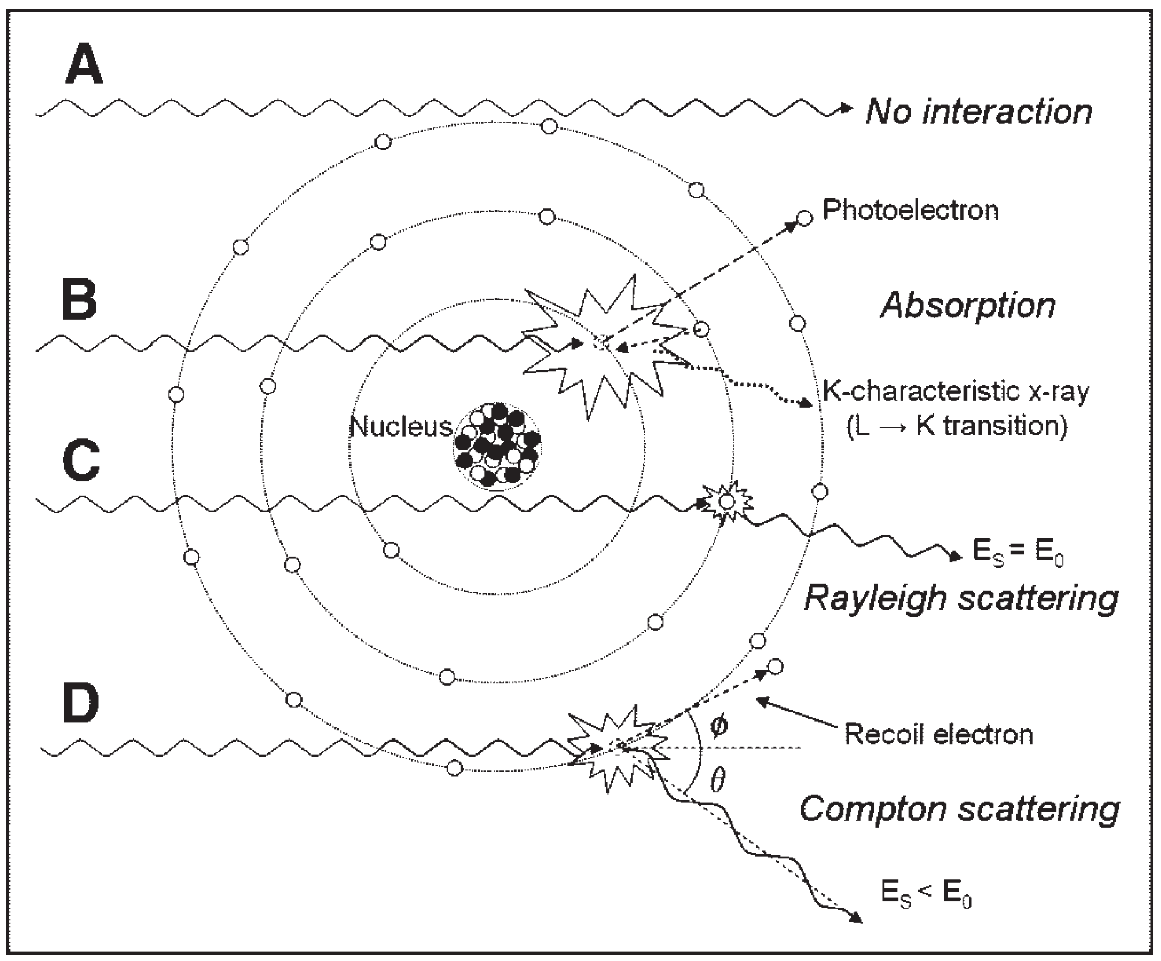
\includegraphics[scale=0.45,angle=0]{2_Theory_Methods/figures/Interactions.pdf}
\caption{Illustration of the described interactions. (A) No interaction resulting in transmission of photon. (B) Photoelectric absorption from inner shell electron, resulting in its ejection and followed by an inner electron transition and characteristic X-Ray emission. (C) Elastic (Rayleigh) scattering conserving the energy of the photons but resulting in small angle change in direction. (D) Compton scattering with outer shell electron resulting to change of energy and direction of incident photon. Adapted from \textit{Seibert et al.}~\cite{Seibert2005}.} 
\label{fig_2:511_interactions}
\end{figure} 
%
\subsection{Attenuation}
Knowledge of the probabilities for interaction of the 511 \si{k\electronvolt} photons in a material can be used to calculate a precise attenuation factor that can be applied at the macroscopic level. Given a well collimated photon beam of intensity $I_0$, the intensity $I_x$ at depth $x$ within the material (along the direction of the beam) will be reduced due to interactions with the material according to Beer-Lambert's law
\begin{equation} \label{Attenuation}
I_x = I_0 e^{-\mu x} \ ,
\end{equation}
where $\mu$ is the linear attenuation coefficient (in cm$^{-1}$). This factor accounts for all possible interactions, whether absorption or scattering, and its value depends on the material properties and the energy of the photons.
%
%Specifically for \gls{pet} where we are interested in the detection of both annihilation photons, the attenuation in the direction of the photon pair can be summed up, resulting in a factor that is independent of the depth of the annihilation and is only depended of the attenuation coefficient of the tissues or materials crossed by the line connecting the two photon detections and the total length of the line within the body, as shown in figure~\ref{fig_2:511_attenuation}~\cite{Phelps1975}. 
%
%\begin{figure} [h!]
%\centering
%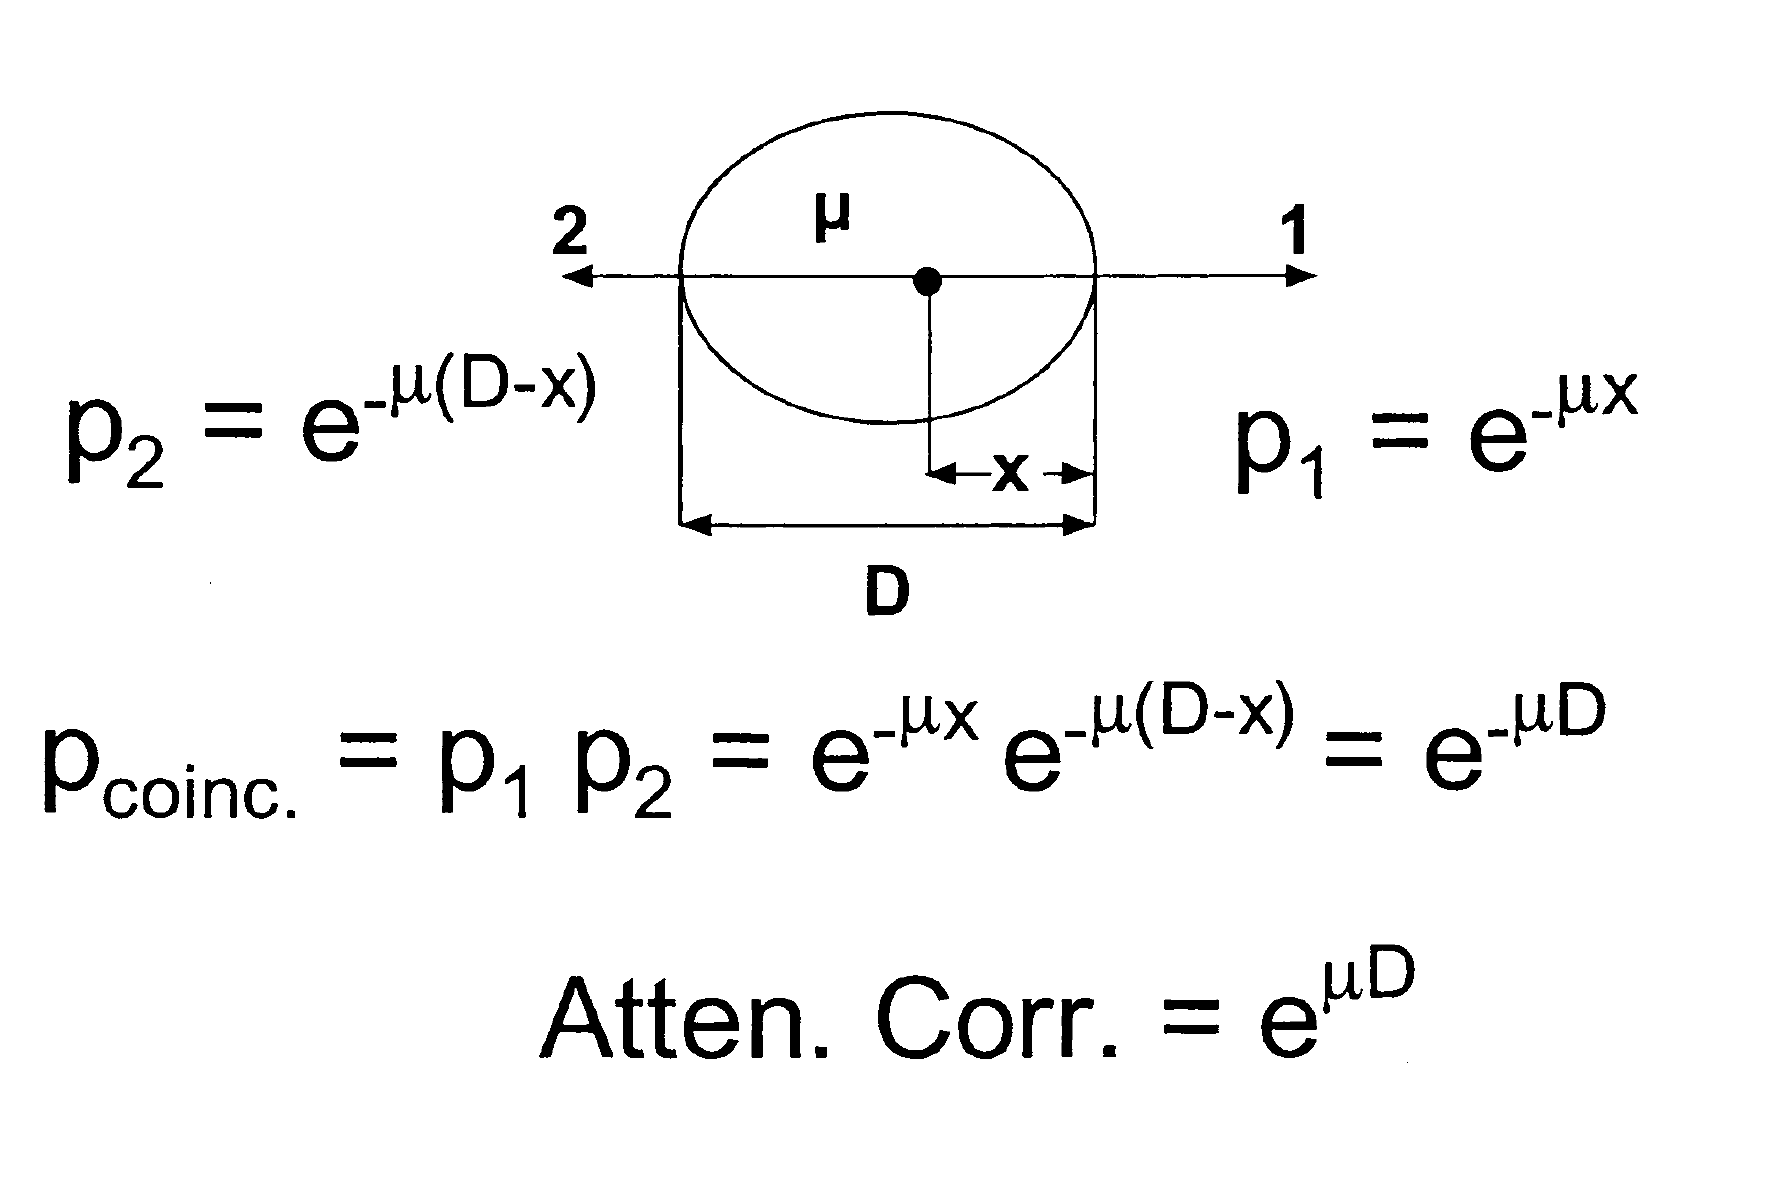
\includegraphics[scale=0.45,angle=0]{2_Theory_Methods/figures/Phelps_LOR_attenuation_correction.png}
%\caption{Attenuation of LORs TODO:  to include in text ! } 
%\label{fig_2:511_attenuation}
%\end{figure} 
%
\section{PET Systems}

\subsection{PET Detectors}
The goal of a PET imaging system is to stop and detect the annihilation photon pairs and record information that can be used to estimate the annihilation event's position.
The basic component for the detection of annihilation gammas is the scintillation crystal. These are inorganic crystals that emit light (lower energy photons) upon interaction with the gammas. The amount of produced light is proportional to the energy deposited by the gamma interactions and can be used to deduce energy information of the interaction. Photosensitive detectors are coupled with the crystals to capture the produced light and output an electronic signal that can be digitally registered. Traditionally \glspl{pmt} are used in most PET systems, while some more recent systems make use of \glspl{sipm}. Depending on their mode of operation \glspl{sipm} can allow for better efficiency and response speed and can be used in conditions where \glspl{pmt} could not, such as within the MR field of PET-MR hybrid systems. More details on \gls{sipm} integration in PET/MR are given in section~\ref{sec:PET_MR_Systems}.
%
%\footnotetext{https://www.radiologycafe.com/radiology-trainees/frcr-physics-notes/pet-imaging}
\begin{figure} [h!]
\centering
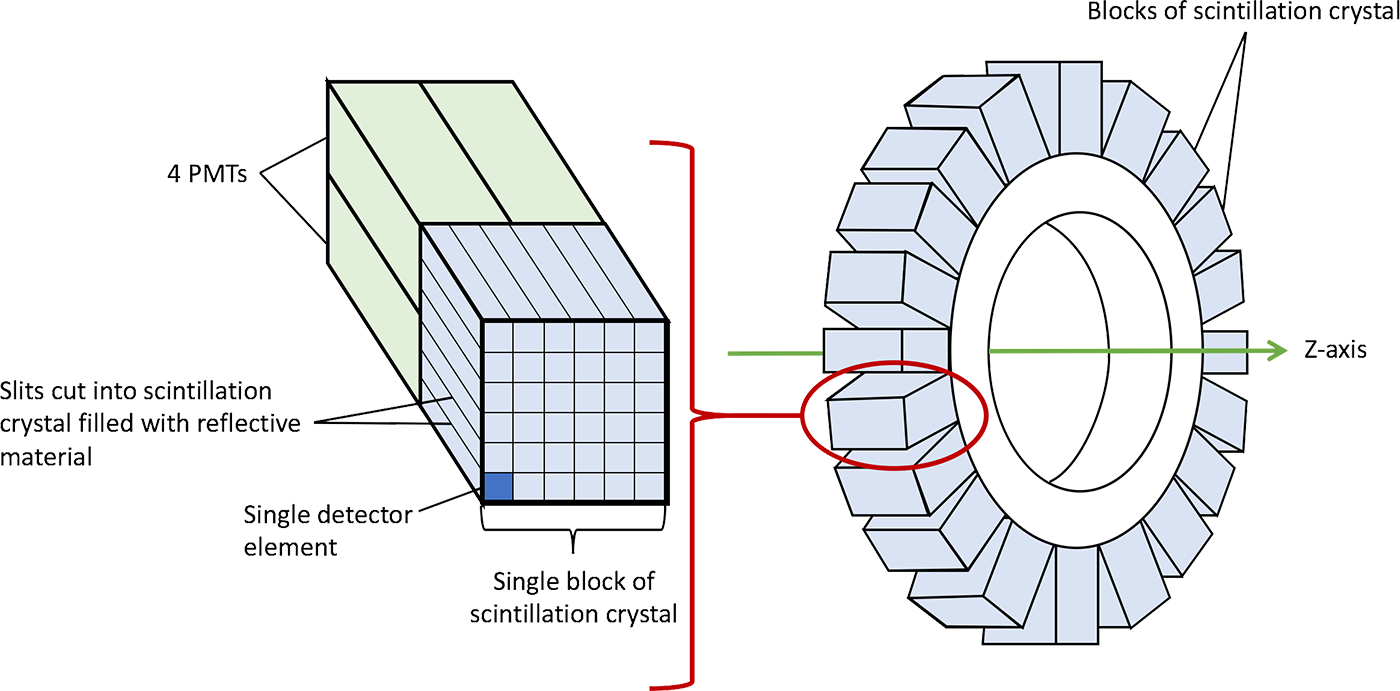
\includegraphics[scale=0.28,angle=0]{2_Theory_Methods/figures/block_detector.png}
\caption{Example illustration of PMT based block detector diagram and their placement within a PET ring (Adapted from www.radiologycafe.com) } 
\label{fig_2:BlockDetectorAndRing}
\end{figure} 
%\begin{figure} [h!]
%\centering
%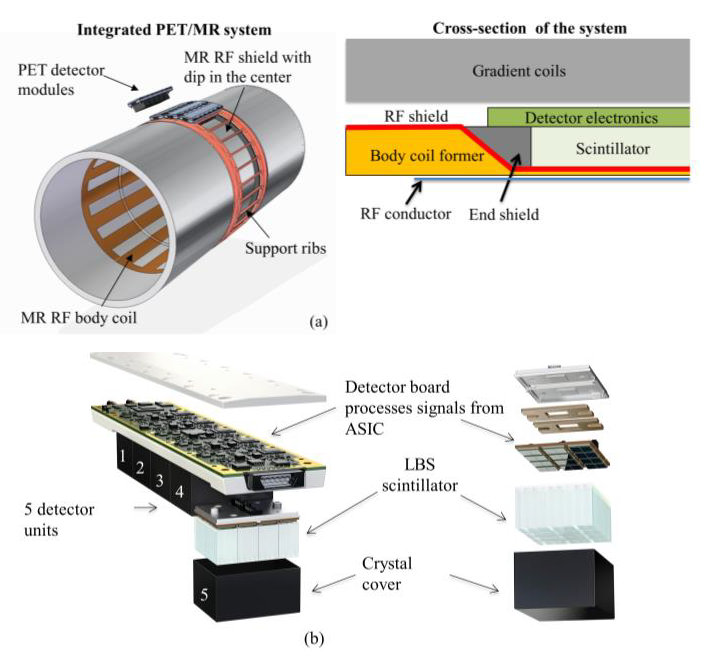
\includegraphics[scale=0.45,angle=0]{2_Theory_Methods/figures/SignaPETMR_Integrated_System.png}
%\caption{Schematic of an hybrid PET-MR system with, comprising of detector module units (bottom) in a ring formation within the MR RF body coil (top)~\cite{Levin2016}.} 
%\label{fig_2:SignaPETMR_Integrated_System}
%\end{figure} 
%%
%
The most common configuration of the PET detectors is within a block or module configuration, where a smaller number of photosensitive detectors to number of crystals is used. An example of a single crystal block to 4 \glspl{pmt} is shown in figure~\ref{fig_2:BlockDetectorAndRing} for PMT based scanners. The crystals are partially cut into segments to reduce lateral dispersion of light and improve localisation of detection by the \glspl{pmt}. In the example of figure~\ref{fig_2:BlockDetectorAndRing} the crystal is cut in a 6$\times$6 configuration.

The blocks or modules are placed in ring configurations that provide full 360$^{\circ}$ of coverage in the transaxial direction. Multiple rings are often placed adjacent to each together to increase axial coverage and solid angle coverage which provides increased detection sensitivity. 

\subsection{PET Data coincidence sorting}
Individual events recorded by the detectors are called \textit{single} events. In \gls{pet} detection of annihilation events requires the detection of both annihilation generated photons. To identify these photons the detection system makes use of "coincidence detection". Pairs of single events detected within a predefined timing window are assumed to be photons originating from an single annihilation, these are defined as \textit{true coincidence events}.
The line connecting the two detectors that record the coincident event is defined as the \gls{lor}. 
%In reality this is a volume of response, that accounts for the volume intersected by the face of the two involved detector elements. But the term~\gls{lor} is used to describe a detection event in PET.

Improved timing resolution of detector systems has allowed for further information of the annihilation point to be made by capturing the arrival difference of the two photons. This difference can help localise the point on the \gls{lor} where the annihilation took place, within some range of uncertainty defined by the detector timing resolution. This capability of PET is refereed to as \textit{time-of-flight} (TOF).
This information, collected for each coincidence event, can then be used within the image reconstruction for imporved results as it will be explained in chapter~\ref{Chap2_3:Reconstruction}.
%Due to uncertainties in the photosensitive detectors which result in timing uncertainly, a timing resolution τ is defined for the system.
%The coincidence timing window is then set at 2τ to sort pairs of events as coincidences.
%As detectors and systems improve on timing resolution it now also possible to record the difference in arrival time between two coincidence photons, owing to the difference in distance travelled from annihilation to detection and the finite speed of light. That difference provides additional information for each detection, refereed to as \textit{time-of-flight} (TOF). This additional information can be used for better positional estimation of annihilation events across the \gls{lor}, as shown in figure~\ref{fig_2:TOF_bin}, resulting in improved reconstructed image quality and sensitivity.
%
%
\begin{figure} [h!]
\centering
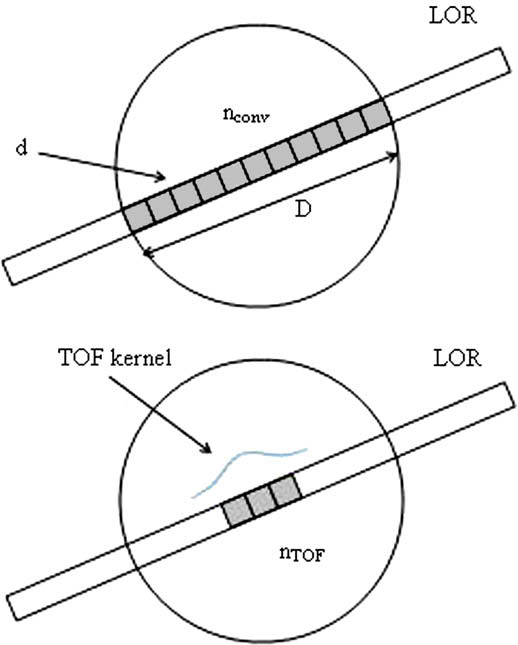
\includegraphics[scale=0.55,angle=0]{2_Theory_Methods/figures/TOF_bin.png}
\caption{Comparison of non-TOF (top) and TOF of annihilation event position across an LOR (bottom)~\cite{Conti2009}.} 
\label{fig_2:TOF_bin}
\end{figure} 
%
Unfortunately not all events recorded within the coincidence window will always be originating from the same annihilation event, they could also be one of the following type of events. 
%
\begin{itemize}
\item\textbf{Random event}\\
As the rate of single events increases the chances of photons originating from different annihilation events being detected within the coincidence timing window are also increasing. These photons will not have interacted with the body before being detected.
In this case the system will record coincidence events that are not correlated. These events are refereed as random events. 
The rate of random events is directly proportional to the size of the timing window and to the square of the activity in the scanner. These events are uncorrelated to the imaged object and hence degrade the acquired data and subsequently image quality and quantification.  
The expected rate of random coincidences can be estimated using the rates of single events or using delayed coincidence windows. These estimations are then pre-processed and subsequently applied as corrections in the image reconstruction process. 
Randoms estimations can be made using the rates of single events or using delayed coincidence windows, which can then be applied as corrections during the image reconstruction process. 
%
%Photons travelling in straight line (no interaction with the body)
%
\item\textbf{Scatter events}\\
As described scattering of the annihilation gammas results in changes to its energy and direction of travel. Subsequent detection of scattered gammas results in mis-positioned \glspl{lor} that also degrade the data, image quality and quantification. 
Because scattered gammas have lower energy than 511 \si{k\electronvolt}, they can be rejected by applying a low energy threshold in the detectors. But due to energy resolution limitations this threshold is set low enough to best avoid rejection of true coincidence events while still filtering a reasonable amount of scattered events.
To correct for the remaining events that are being recorded as true coincidences, special scatter simulation algorithms are employed to estimate the amount of scatter coincidences in the data and account for it during the image reconstruction process~\cite{Watson1996,Polycarpou2011}.

\item\textbf{Multiple events}\\
Multiple single events (more than two) can be are recorded within the coincidence timing window in which case they are refereed to as a multiple event. As these cannot be used to resolve \glspl{lor}, they are either rejected completely or in some cases further processed to deduce which pair of single events are more likely to  be true coincidences using techniques that vary between scanner models and manufacturers. 

\item\textbf{Delayed event}\\
As described above, an estimation of randoms can be made using an additional detection channel to capture coincidences with a delay of several times the duration of the coincidence window. These events are considered uncorrelated and serve as an direct measurement of randoms. Specific variance reduction techniques are then applied on these randoms estimations before being used as corrections in reconstruction, to avoid inducing additional noise in the data~\cite{Bailey2005}.

\item\textbf{Prompt event}\\
True, random and scatter events that meet the acceptance criteria for detection are indistinguishable at the time of detection and recorded as valid coincidence events. They are refereed to as prompt events.
These are pre-corrected or used directly in the reconstruction process along with the corrections, depending on the use of either analytical or statistical reconstruction methods respectively.
\end{itemize}
%
\begin{figure} [h!]
\centering
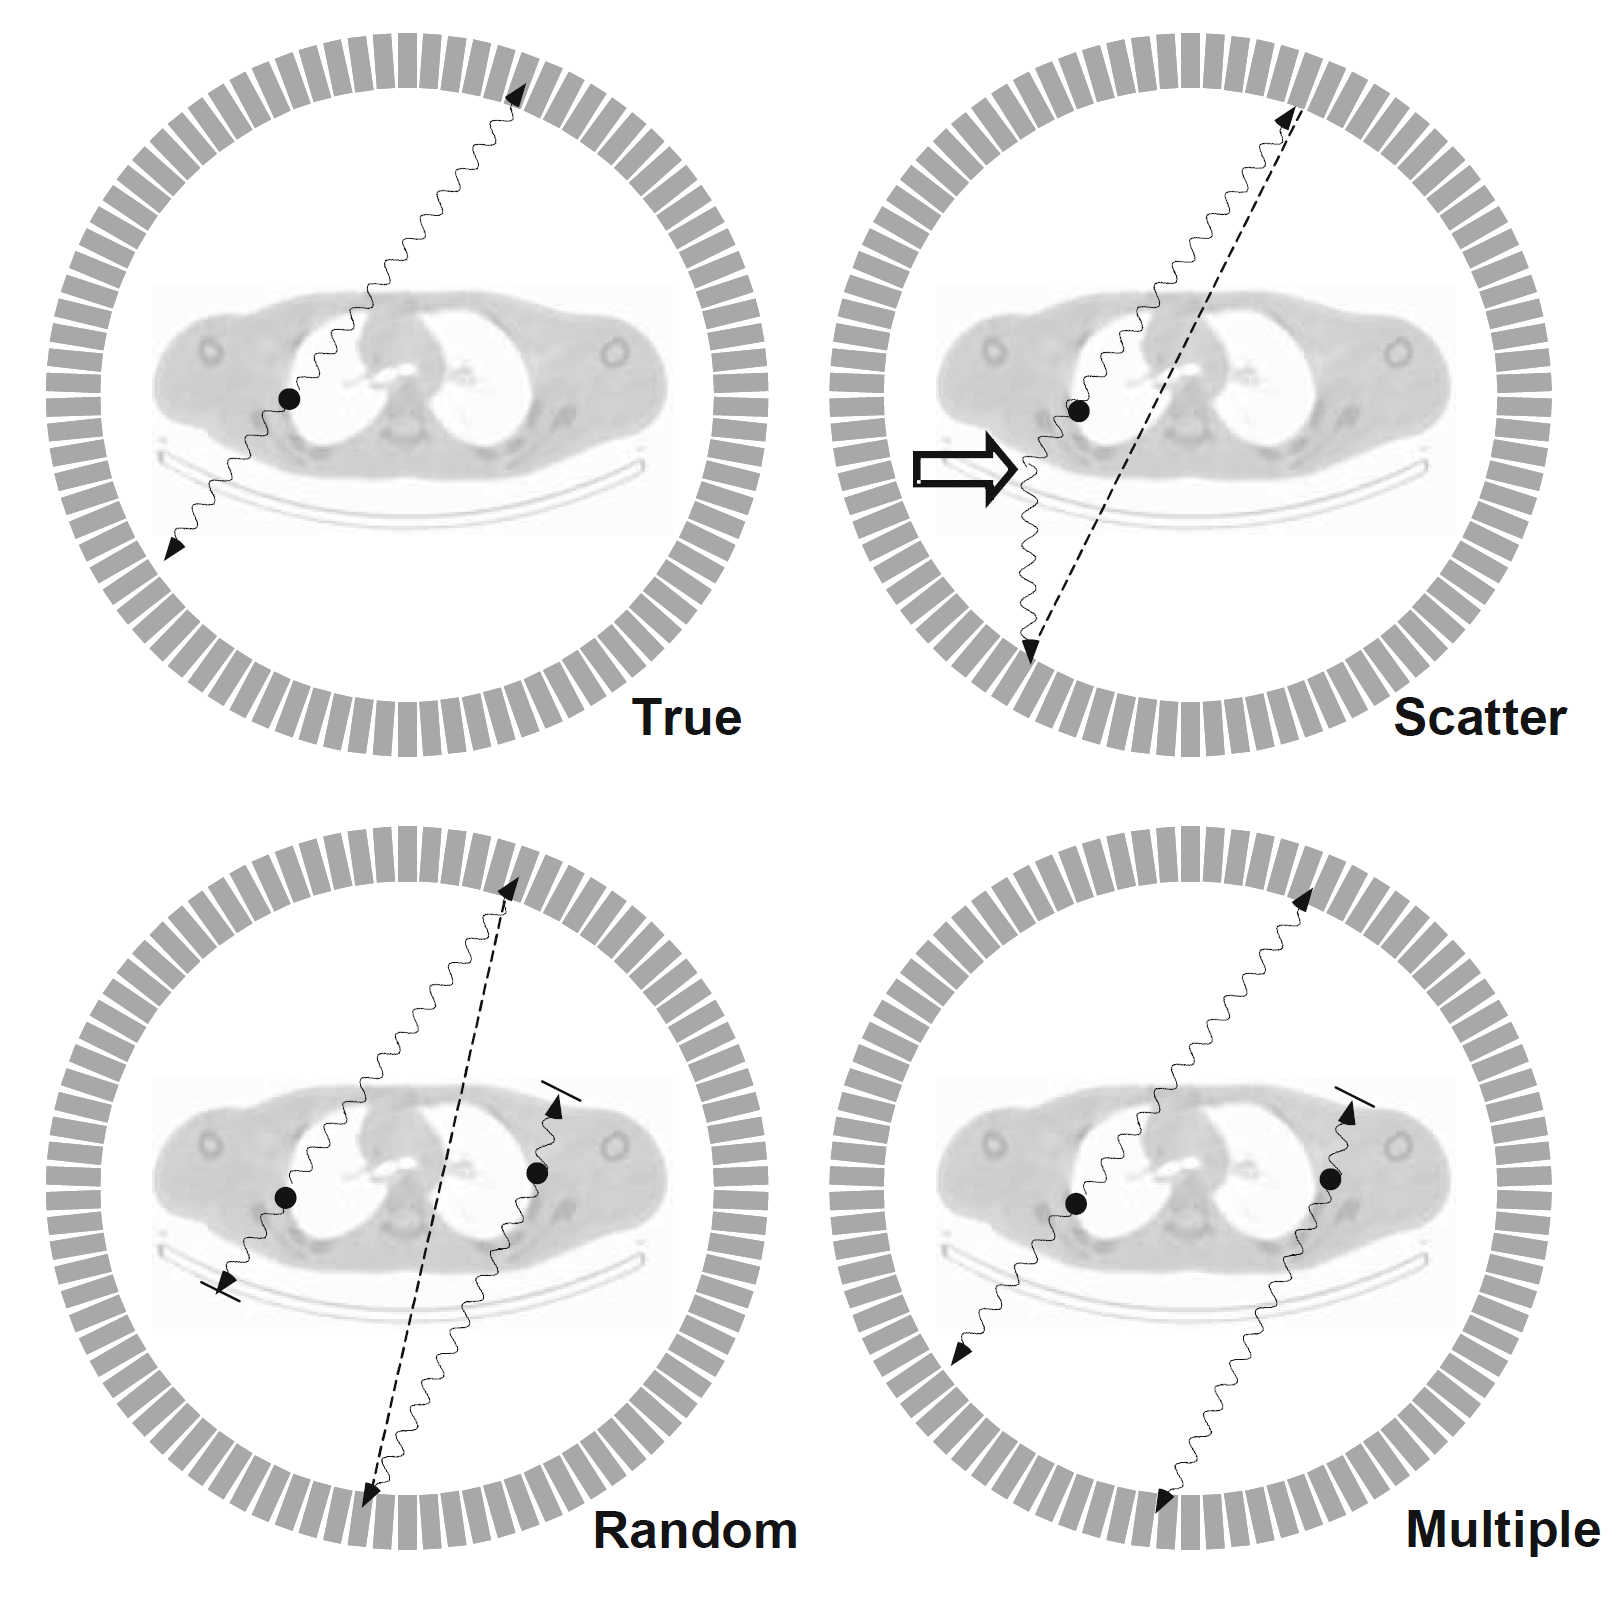
\includegraphics[scale=0.22,angle=0]{2_Theory_Methods/figures/Bailey_Scatter_Random_events.png}
\caption{Representation of different types of detected coincidence events. Adapted from Bailey~\textit{et al.}~\cite{Bailey2005}.} 
\label{fig_2:EventsIlustration}
\end{figure} 
%
%
\subsection{PET acquisition}
As described the ring formation of PET detectors is the dominant geometry used in PET systems. Using multiple rings results in increase of \gls{afov}, solid angle coverage and possible combinations of detectors meaning higher number of ~\glspl{lor}. But early multi ring systems were making use of 2D acquisition, where only direct and cross-plane ring coincidences were allowed. 
This was enforced using tungsten septa between rings, as seen in figure~\ref{fig_2:2D3D}. The use of cross-planes allowed for the increase in axial resolution and the septa result in an uniform axial sensitivity profile as seen in figure~\ref{fig_2:2D3DSensitivityProfiles}.

With evolving detector and electronics technology, 3D acquisition became possible and is now the standard acquisition mode. 3D acquisition offers the same data as 2D acquisition but also includes all the oblique \glspl{lor} data resulting in an increase of sensitivity (4 to 6 times)~\cite{Fahey2002}. The use of oblique views leads to non-uniform sensitivity profiles in the axial direction due to the higher number of \glspl{lor} closer to the center of the \gls{afov}, with the maximum sensitivity at the centre and a minimum at the edges of the \gls{afov}. A comparison between the 2D and 3D sensitivity on the same 45 direct planes is shown as an example in figure~\ref{fig_2:2D3DSensitivityProfiles}.
In addition to more coincidence events, the higher sensitivity and acceptance of single events results to an increase of randoms and scatter events, which in addition may now be originating from activity outside the \gls{afov} of the system. 
%
\begin{figure} [h!]
\centering
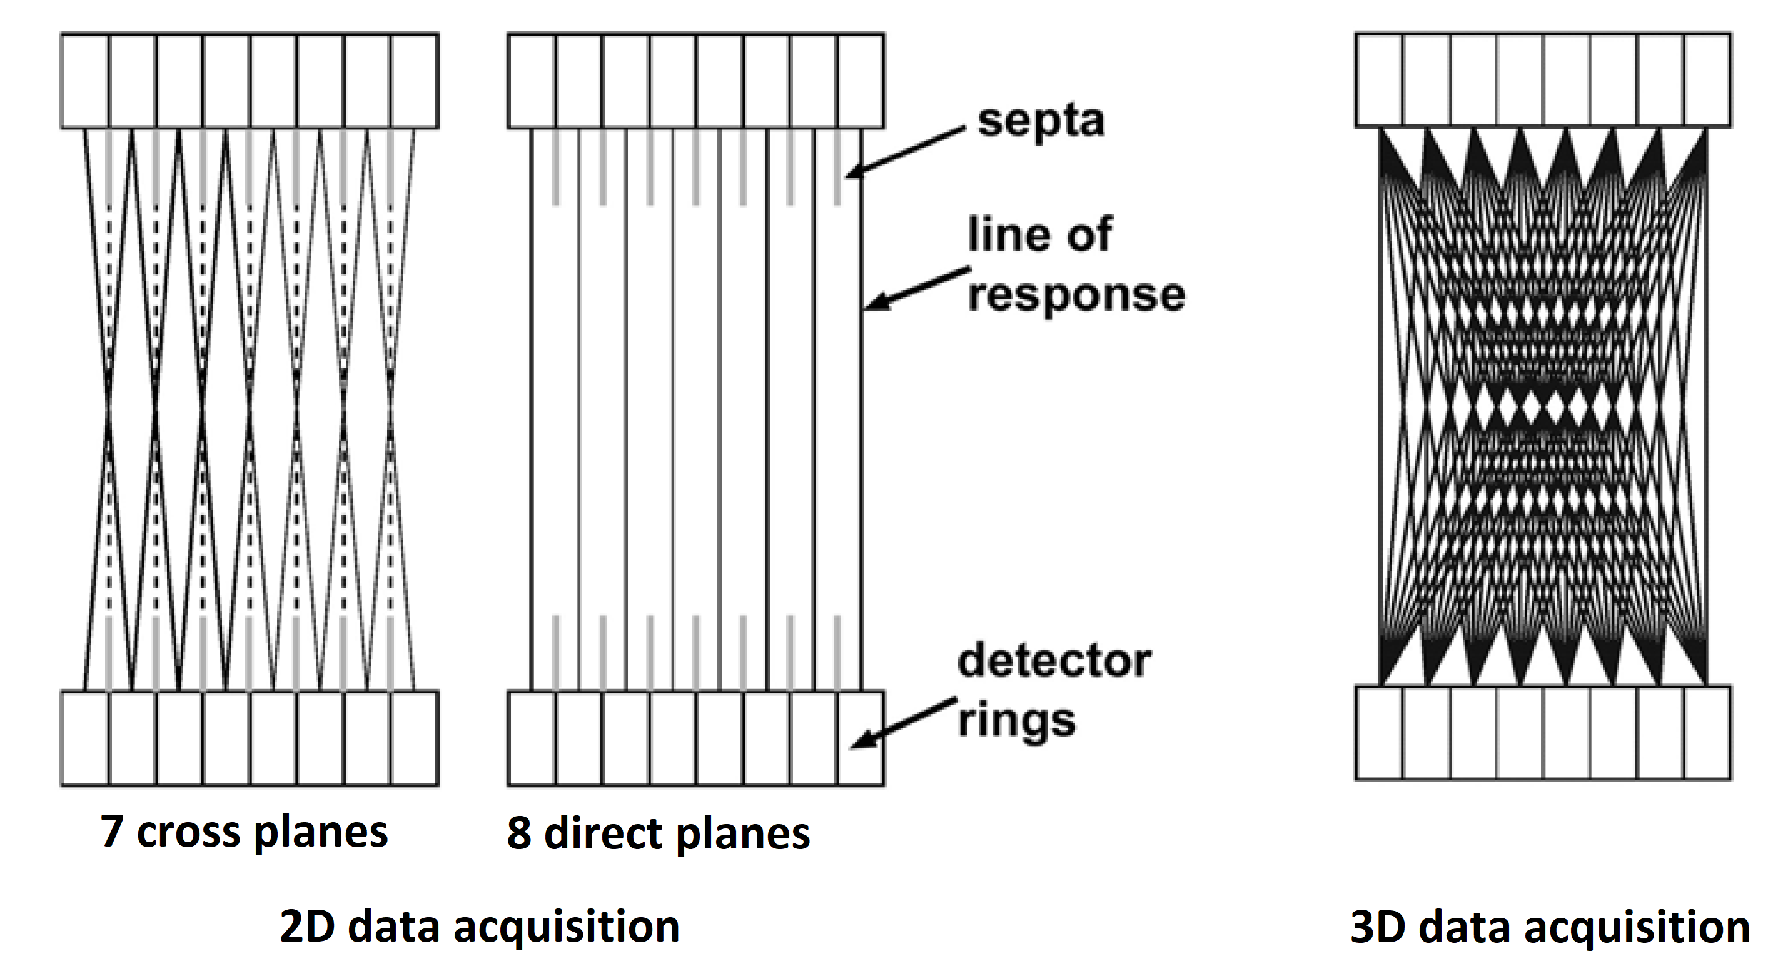
\includegraphics[scale=0.40,angle=0]{2_Theory_Methods/figures/Phelps_2D_3D_Acquisition.pdf}
\caption{Example illustration of LORs for 2D acquisition mode using direct and cross planes (left) and 3D  acquisition mode (right) for an 8 ring scanner with 15 axial slices. Adapted from Cherry S. and Magnus D.~\cite{cherry2004pet}} 
\label{fig_2:2D3D}
\end{figure} 

\begin{figure} [h!]
\centering
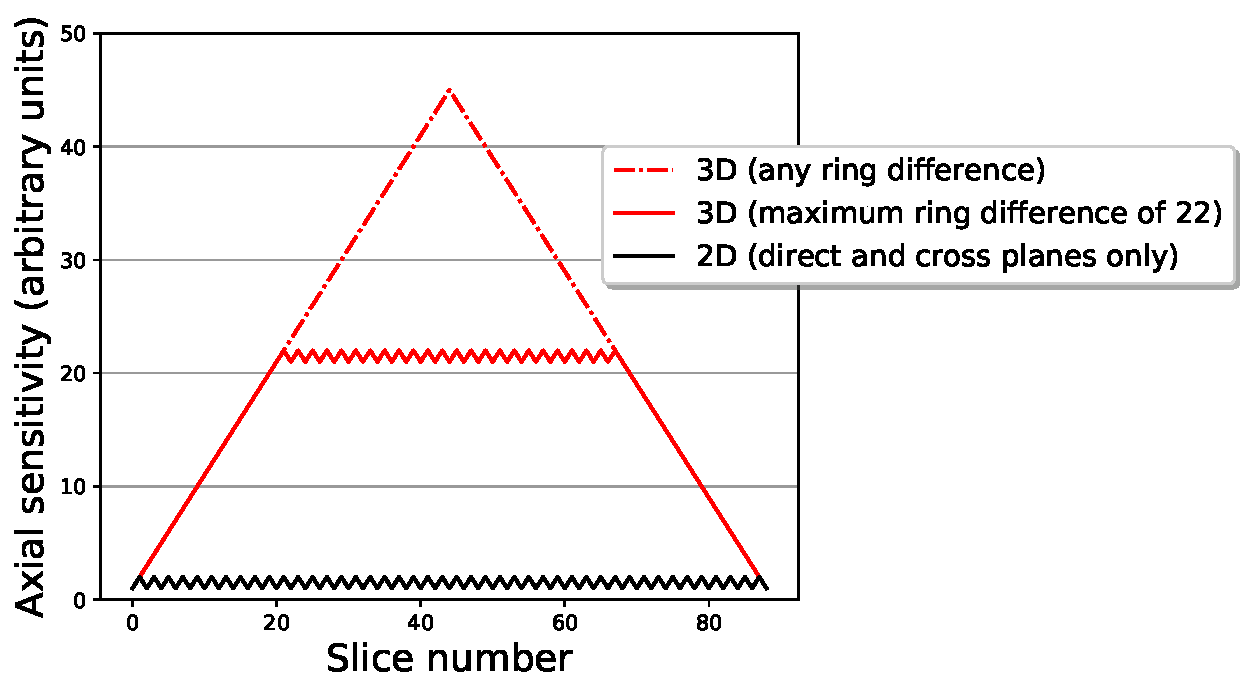
\includegraphics[scale=0.50,angle=0]{2_Theory_Methods/figures/2_2_2D3DSensitivityProfiles.pdf}
\caption{Example of 2D and 3D axial sensitivity profiles, with and without maximum ring difference limits, for a scanner with 45 direct planes which provides 45 direct and 44 cross-plane.} 
\label{fig_2:2D3DSensitivityProfiles}
\end{figure} 
%
%
In 3D mode the maximum angle of events accepted in the axial direction can be sometimes limited by enforcing a maximum ring difference permitted \glspl{lor}. This results in a uniform axial sensitivity profile at a central region of the \gls{afov}.
%
%In multiple beds acquisition, used to image objects with a length larger than the scanner \gls{afov}, in order to maintain an uniform axial sensitivity a degree of overlapping is used. This allows for the regions at the edges of the bed positions to be sampled in two bed acquisitions and even out the sensitivity of the combined acquisition. The degree of overlapping can vary, depending on requirements of sensitivity uniforming and speed of acquisition.
%
\subsection{Storage of PET coincidence events}
The recorded coincidence data are stored digitally to allow post processing and reconstruction of image data.
The different methods for storing the data can result to different storage requirements, allow or not allow for specific event information to be stored and even necessitate different reconstruction techniques. 

\begin{itemize}

\item\textbf{List Mode}\\
In the simplest form coincidence events can be stored in a binary file as a stream of events by the order of their detection. This format follows naturally the detection process and allows for multiple detector information to be included in each event. A time tag is normally included in the data stream every millisecond. The minimum information recorded per event is the detector pair IDs. Any additional information such as time-of-flight, detection energy, etc. can also be included with each event. Additionally for time-of-flight the data can include exact arrival time differences, to make best use of the information instead of binning the ToF as done in the histograms described bellow.
The use of list-mode files is practical for dynamic studies as they takes less storage space than the other alternative formats described bellow, and furthermore they allows for subsequent re-binning into any required temporal framing. Reconstruction algorithms can be derived to reconstruct data directly using the list-mode stream.

\item\textbf{Histogram}\\
Coincidence events per detector pair (\gls{lor}) can be summed together and stored into a single entry. The total number of entries will be equal to the total number of detector pairs. These entries make up a histogram, where effectively all the events have been histogrammed into the detector pairs. No timing information is preserved and hence multiple histograms are required if data are recorded dynamically, in a predefined temporal binning. 
This format can result in smaller files for static imaging compared to list-mode, but in the case of dynamic imaging it frequently results in much larger total size of files as multiple detector pair entries are empty (zero) for some time frames. Furthermore if time-of-flight information is also available, separate histograms need to be created for each time-of-flight bin (discretization of the TOF resolution), which further increases the zero entries and storage requirements. 
Compression is possible in both axial and transaxial direction of the data, refereed to as axial compression (or span) and angular compression (or mashing) respectively~\cite{Fahey2002}. These are employed by some scanner manufacturers to counteract the increasing size of histograms from increasing scanner resolution and better TOF resolution. The compression strength is chosen as a trade-off of file size and degrading image quality properties~\cite{Belzunce2017}. 

\item\textbf{Sinogram}\\
Sinograms are representations of the data in projections though the process of projection using a transformation such as the radon or X-Ray transform~\cite{Natterer1986}. Each pixel of the sinogram represents the integral of events over a specific line though the image space. The name "sinogram" comes from the fact that a point source (off-centred) is represented as a sine wave in the sinogram.
Use of sinograms is inherited from other tomographic imaging methods where data are acquired as projections. Sinograms are used with analytical reconstruction methods, shortly described in chapter~\ref{Chap2_3:Reconstruction}, which require the projection space to be fully and uniformly sampled.
%In \gls{pet}, contrary to list-mode and histograms where the data are directly related to detector elements, conversion of data to sinograms requires certain processing steps to ensure 
%As seen in figure~\ref{fig_2:Sinogram_detector_to_Sino}, parallel \glspl{lor} at a specific direction are used to form the sinogram along a particular row. The sampling of the sinogram space will depend on the size of the sinograms required, and data conversions will be required  to match the required sinogram sampling \cite{Fahey2002}. 
%
%\begin{figure} [h!]
%\centering
%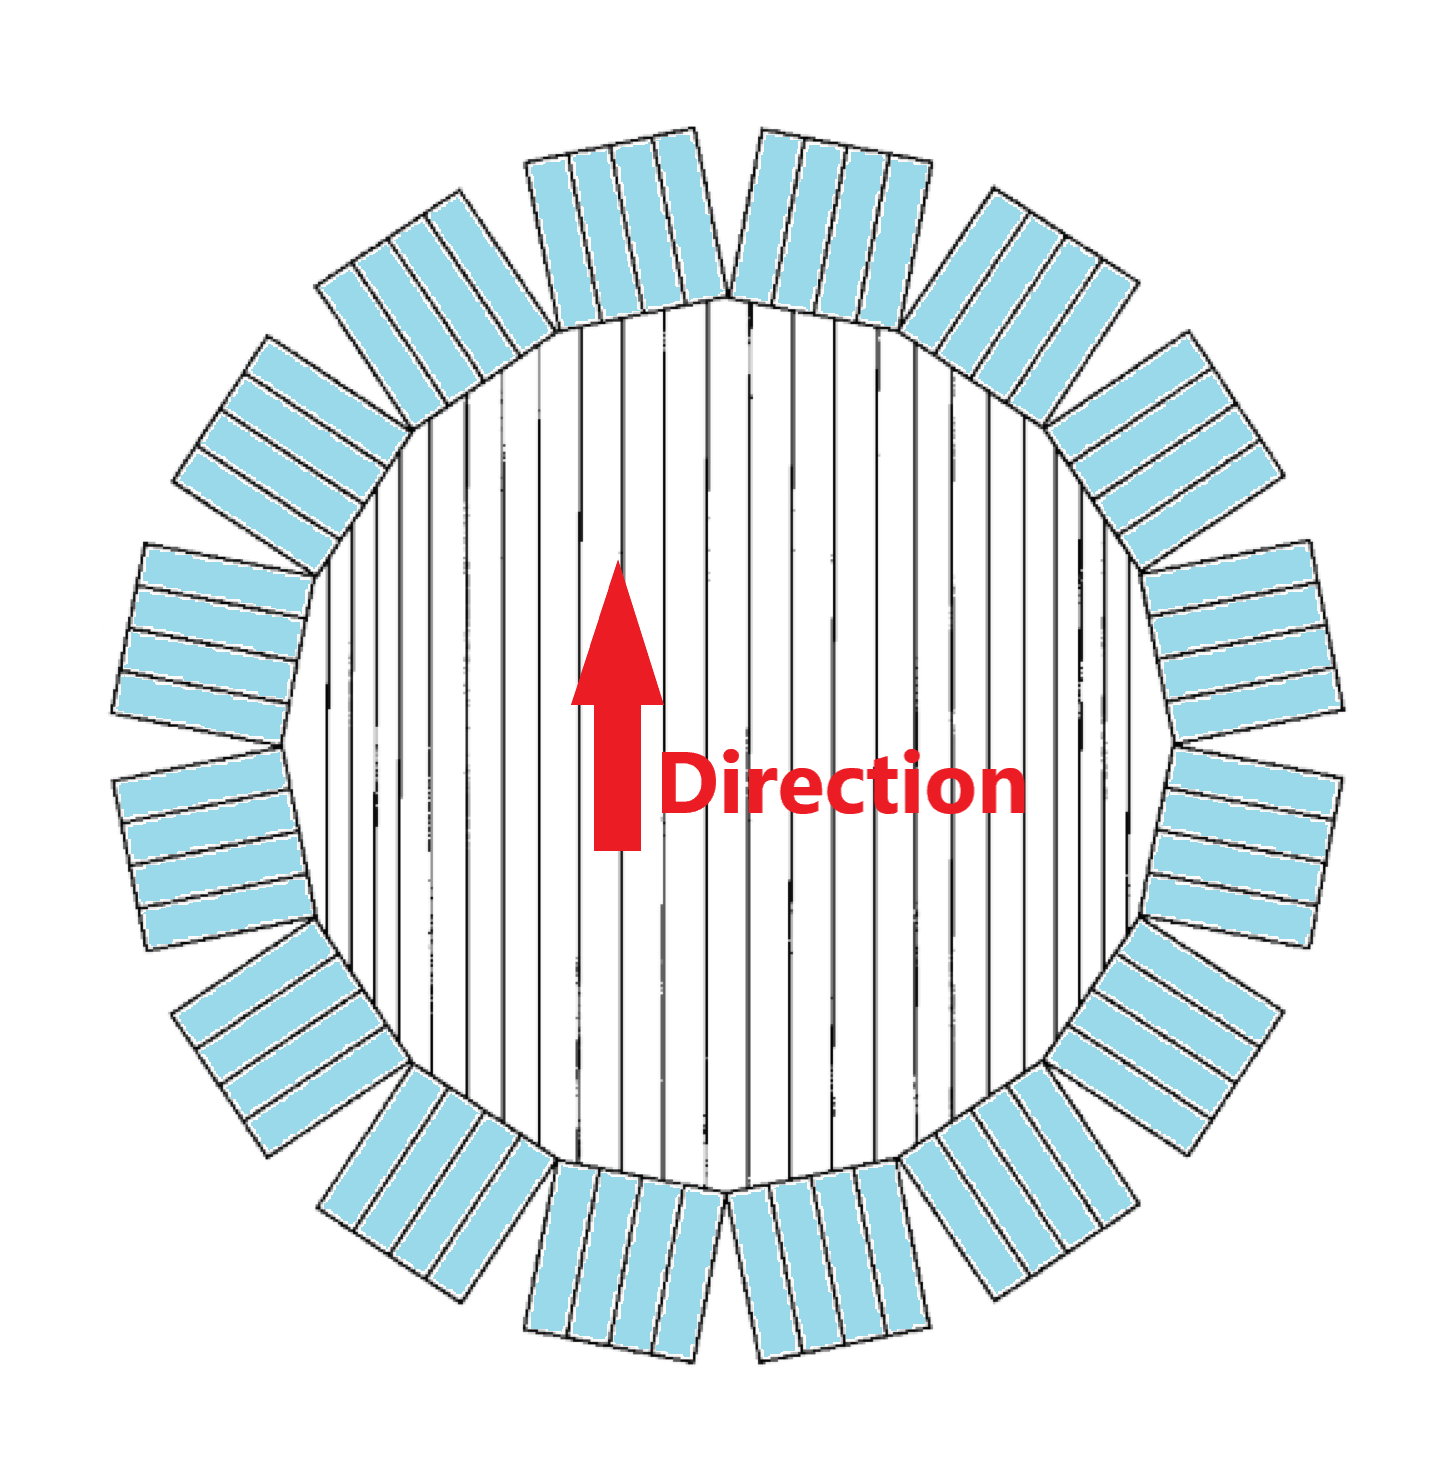
\includegraphics[scale=0.15,angle=0]{2_Theory_Methods/figures/Sinogram_detector_to_Sino.png}
%\caption{Example projection though the PET field of view for a specific direction~\cite{Fahey2002}.} 
%\label{fig_2:Sinogram_detector_to_Sino}
%\end{figure} 
%
%In practice events can be detected in any angle within the transaxial plane as well as the axial planes that are defined by the multiple detector rings that form the \gls{pet} system. In 3D acquisition, crystals from all rings (or under certain maximum ring difference limitations) are allowed to record coincidences. In this case the number of sinograms increases to allow all the possible co-planar angle combinations, and the radon transform is extended in 3D. With the introduction of time-of-flight information, a separate set of sinograms is required for each TOF bin and when dynamic data are captured a separate set per temporal bin. In practice different types of compression have been used to reduce the total size of sinogram raw data.
\end{itemize}

As in this project we did not make use of analytical reconstruction algorithms, we have not described the formation and use of sinograms in detail. 
In the project we made use of both real data from clinical PET scanners and simulated data from analytical simulations. For real data we made use of the list-mode data format, to reduce file size and allow for flexibility in treatment of the data, while for simulations we used the histogram data format as we were limited to that by the nature of analytical simulations.
It is important to note that clinical PET systems are performing reconstructions using histograms or sinograms and although they can record data in list-mode format, they always re-bin the data to histograms or sinograms before performing a reconstruction. 
By contrast in this project we made us of list-mode reconstruction algorithms when using list-mode datasets.

\subsection{PET Corrections and Quantification}
PET has always been used as a quantitative imaging method, providing image values that relate to radioactivity concentration. This is important for semi-quantitative and quantitative interpretations of the imaged data, with quantitative measures being at the foreground on this thesis project.
But accurate quantification of images requires corrections that need to be considered before and during the reconstruction process. The main corrections needed for quantifiable PET our outlined here.

\begin{itemize}
\item\textbf{Randoms correction}\\
As discussed previously, random events in the data are estimated using delayed coincidence detection or by measurements of single event rates between detectors. For most clinical scanner manufacturers and for list-mode data these are normally provided in the same stream of data, with delay events recorded similarly to prompts and with single events recorded for every pre-defined time interval (for example every second) for each detector or detector block. Similarly, for histogram data a separate histogram of random events is provided. A histogram per frame (time bin) is required for multiple frame datasets, for randoms as well as for prompt events. 
In the reconstruction software used in this projects, \gls{castor}~\cite{Merlin2018}, the corrections are provided for each event \gls{lor} or histogram within the raw dataset file. Furthermore, randoms corrections in \gls{castor} are provided in rates (s$^{-1}$) which is a more natural format to use with list-mode data reconstruction and dynamic datasets.
\item\textbf{Scatter correction}\\
As described previously, a certain amount of the annihilation gammas will scatter with the atoms of the travelling medium via Compton scattering, which results in changes of energy and direction of the gammas. Even after energy filtering applied on the detectors, an amount of those scattered gammas will be detected and recorded as coincidence events and degrade the PET data and affect image quality and quantification. The most commonly used approach to account for scatter in clinical scanners is the use of the Single Scatter Simulation algorithm~\cite{Watson1996} to estimate scatter. These simulations are based on an initial activity distribution estimate from the uncorrected PET data and knowledge of the probability of scattering. 
Scatter estimates, similar to random estimates, are used as additive corrections within statistical reconstruction methods. Again, in~\gls{castor} these are provided as \mbox{rates (s$^{-1}$)}. 
\item\textbf{Normalisation}\\ 
Sensitivity between \glspl{lor} will be different due to detector and geometric efficiencies effects. Normalisation coefficients for each \gls{lor} are estimated using measurements and modelling of the normalisation components and are subsequently used in reconstruction to correct for these efficiencies.
\item\textbf{Dead-time correction}\\
After every detection event a certain amount of time is required for sub-systems involved in the detection to become ready for detection again and so interaction events occurring during that recovery time will not be registered. As the number of interactions increases at higher imaged activities, the proportion of events not registered is also increasing. This results is a non-linear system response for different levels of imaged activities. This effect is corrected using dead-time correction which is applied by the of lookup tables that relate single rates to dead-time factors and real-time singles monitoring measurements.
\item\textbf{Attenuation correction}\\
Absorption or scatter interactions within the body result in loss of gammas detection. Even if one of the two annihilation gammas is lost the result is a non registered event and so the probability of attenuation depends on the total probability of interaction within a \gls{lor} and is independent of the annihilation position within that line. This enables the estimation of attenuation factors for each \gls{lor} within the body by use of transmission measurements, either with radioactive sources or X-rays sources. For these measurements earlier scanners made use of positron or single gamma sources to estimate attenuation while most modern clinical systems make use of \gls{ct} or \gls{mr} scans to estimate attenuation factors. 
\item\textbf{Calibration Factor}\\
%Contrary to other nuclear medicine techniques, \gls{pet} is fully quantitative and can be used to deduce absolute activity measurements from the reconstructed image data. 
Finally, after all other corrections have been applied there is a need for a global calibration factor to relate the estimated number of true events to activity concentration. 
PET systems are calibrated against a reference source to obtain such factors. 
\item\textbf{Decay correction}\\
Finally, measurements need to be corrected for decay of the imaged radionuclide for the duration of the acquisition and for decay-correction to a reference time. 
For static imaging the reference time is chosen to be the imaging start time, while for dynamic acquisitions the reference time is commonly chosen to be the time or tracer injection. 
\end{itemize}

\section{Hybrid PET Systems}
\subsection{PET-CT}
As described above attenuation correction is essential for quantitative \gls{pet} imaging. Early \gls{pet} systems made use of external radioactive sources to acquire a transmission scan. Those would be either positron sources or single photon sources. Some of the drawbacks of these methods were that transmission scans would contribute to an increase of image noise on PET images and that transmission scan acquisition was increasing the total duration of the examination.
As PET imaging became more frequently used in clinical applications, the need for fusion of PET images with CT images became apparent, firstly for the clinical value by complementary PET functional images to CT anatomical images and secondly for aiding in attenuation correction and anatomical localisation. These needs led to the development of first hybrid PET systems, with the first PET/CT system being introduced in late 1990s~\cite{Townsend2008}.
The first PET/CT was able to acquire a whole body PET/CT scan, using multiple bed positions as it will be described later in this chapter, within an hour with precisely co-registered CT and PET images that were acquired close in time~\cite{Beyer2000}. The CT scan was also used for PET attenuation correction via scaling of attenuation factors that were measured for the CT X-ray energy to \si{k\electronvolt} of annihilation photons~\cite{Kinahan1998}. PET/CT eliminated the need for radioactive source transmission scans and the problems with excessive noise associated with these relatively poor quality transmission images.

\subsection{PET-MR}
\label{sec:PET_MR_Systems}
MRI provides anatomical images with higher soft-tissue contrast than CT imaging. The option of different acquisitions sequences can allow for different types of soft-tissue contrast in MR imaging, which can also extend to dynamic and parametric MR imaging applications~\cite{Besson2020} and also to functional MRI~\cite{Kolb2012}.
The fusion of PET and MR was technicaly challenging due to interference between the two systems~\cite{Disselhorst2014}.
Initial PET and MR clinical workflows and systems made use of separate PET and MR or PET/CT and MR scanners to scan the patient using the same bed to transfer from one scanner to the other and minimise patient misalignment~\cite{Zaidi2011,Veit-Haibach2013}.

The use of PMT based detectors for synchronous PET/MR imaging was only possible using long optical fibers that shifted the detection of events by the PMTs at a safe distance away from the centre of the magnetic field~\cite{Shao1997,Mackewn2010}. Later advancements in PET detector technology allowed for Avalanche photodiodes (APD) and silicon photomultipliers (SiPM) based detectors, which led to the development of PET inserts~\cite{Kolb2012} for MR and development of fully integrated PET-MR systems that perform synchronous acquisitions~\cite{Delso2011,Grant2016,Levin2016}.

There are currently two PET/MR integrated systems by commercial manufacturers, the Siemens mMR and the GE Signa. In this project we relied on access and real PET data from a GE Signa PET/MR that is available in our centre. But we also made use of Siemens mMR data in a collaboration project with the Medical University of Vienna that is described in the Secondary Contributions section at the end of this manuscript. 

The Signa PET/MR scanner was designed based on an existing 3 Tesla MR scanner (3T MR750w MR scanner) that was modified to accommodate the PET detector ring. The ring comprises of 28 modules with 720 lutetium based scintillator crystals per module. Those were coupled with SiPM detector modules, which are capable of capturing TOF information. A schematic of the modules and their integration in the system ring is shown in figure~\ref{fig_2:SignaPETMR_Integrated_System}. The PET ring provides a total of 89 slices and an \gls{afov} coverage of approximately 25 cm with slice thickness of 2.78 mm.

\begin{figure} [h!]
\centering
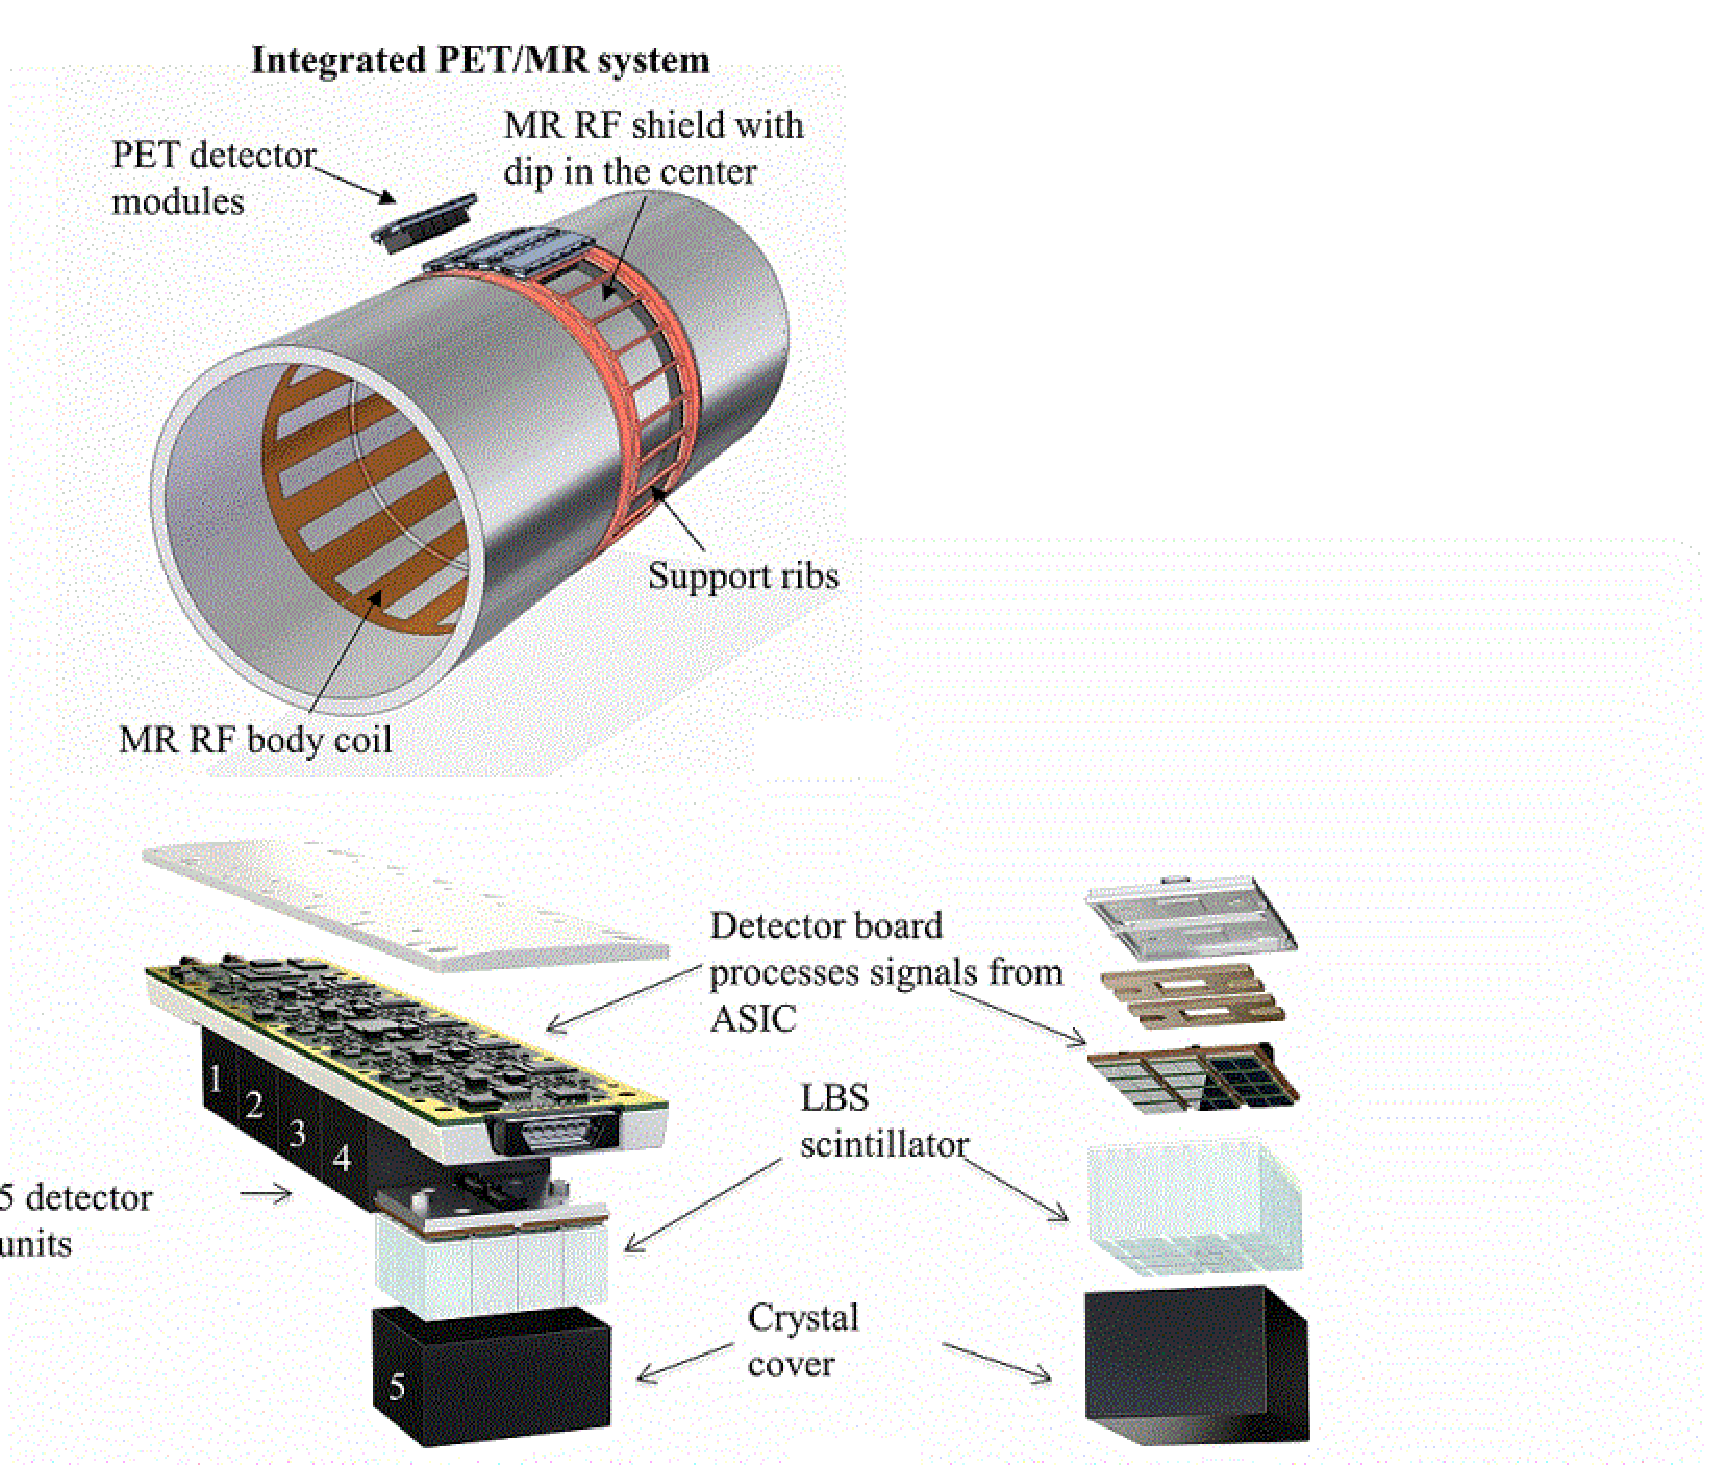
\includegraphics[scale=0.45,angle=0]{2_Theory_Methods/figures/SignaPETMR_Integrated_System.pdf}
\caption{Schematic of the GE Signa hybrid PET-MR system, comprising of detector module units (bottom) in a ring formation within the MR RF body coil (top)~\cite{Levin2016}.} 
\label{fig_2:SignaPETMR_Integrated_System}
\end{figure} 

\section{Whole Body PET: Static Imaging}
For many clinical applications, as for example in oncology, PET imaging over the whole body is essential for detection and characterisation of primary and metastatic disease. Developments in PET detectors technology and reduction of production costs has resulted in increasing axial length of PET scanners using additional detector rings, with currently widespread clinical models offering between 15 to 26 cm of axial coverage~\cite{Vandenberghe2020}.
In practice for static imaging whole-body coverage is achieved using multiple bed positions. The first suggestion and optimization work in extending the effective A-FOV of PET scans using multiple bed positions was by made by Dahlbom~\textit{et al.}~\cite{Dahlbom1992}. This work was made on PET systems operated in 2D mode, where a bed displacement of approximately equal to the system's A-FOV was used to increase the acquisition's effective A-FOV. As systems became capable of acquiring in 3D mode, offering increased sensitivity but resulting in axial varying sensitivity profiles, different strategies were needed for multi-bed acquisitions. The two methods suggested and developed are the \textit{Step and Shoot} (SS)~\cite{Schubert1996} and the \textit{Continuous Bed Motion} (CBM)~\cite{Panin2014} acquisition methods.

\subsection{Step and Shoot}
\label{WB_Static_SS}
The SS method makes use of multiple bed positions that are partially overlapped in the axial direction to increase the sensitivity of the acquisition at the edges of adjacent beds, by combining data of adjacent beds over the overlapping region as shown in figure~\ref{fig3_1:fullOverlap}. 
One way of combining the multi-bed datasets is to reconstruct each bed individually, displace the reconstructed images according to their axial location and combine them using weighted averaging~\cite{Schubert1996}. This method has prevailed in clinical PET systems that use the SS acquisition method, as it does not require addition considerations in the reconstruction process of each bed and the combination of bed images can be performed post-reconstruction. Alternatively the axial displacement of each bed raw dataset can be performed during the projection and back-projection process in iterative reconstruction, which then directly results in the reconstruction of the whole-body image~\cite{Ross2004}. Use of the overlap data in iterative reconstruction can potentially result to improved noise characteristics at the overlapping regions, as the full sampled statistics over these regions are combined prior to each image update~\cite{Ross2004,Stute2014}. 
%
\begin{figure} [ht!]
\centering
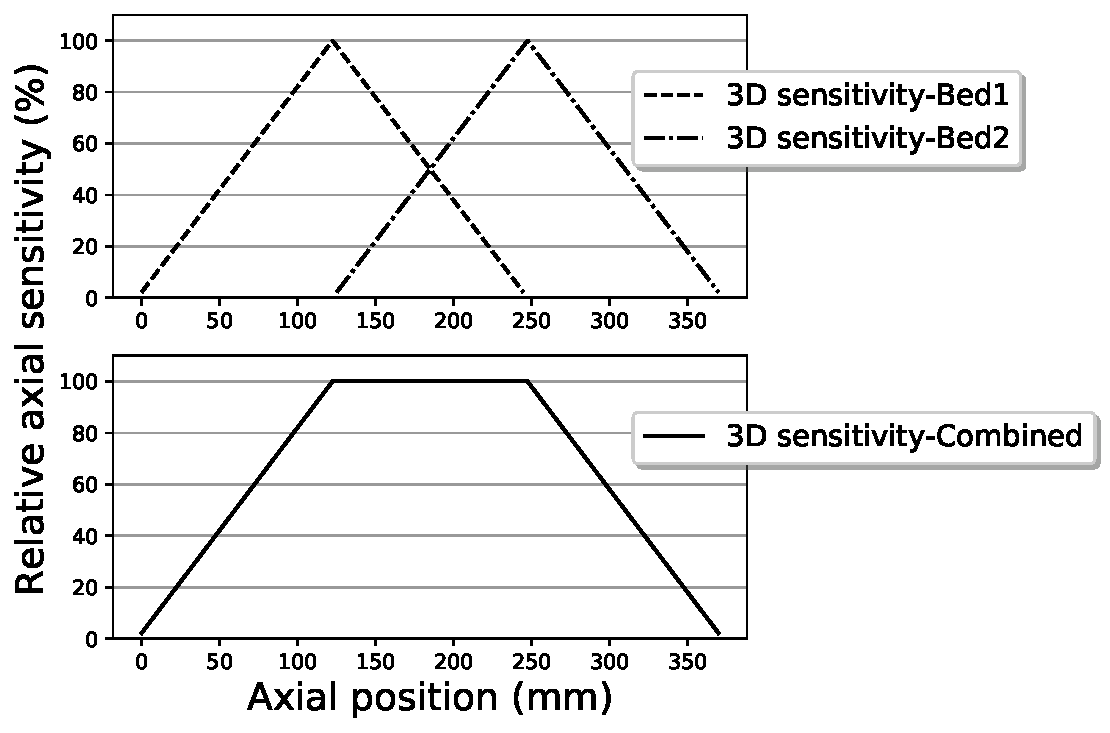
\includegraphics[scale=0.6,angle=0]{2_Theory_Methods/figures/SensitivityProfiles_fullOverlap.pdf}
\caption{Relative axial sensitivity of individual beds (top) and combined sensitivity profile (bottom) for approximately 50\% overlap for the Signa PET/MR.}
\label{fig3_1:fullOverlap}
\end{figure}
%
%The amount of overlap is a parameter to select according to the needs of the axial sensitivity profile.
The axial sensitivity profile for the Signa PET-MR system is shown in figure~\ref{fig3_1:fullOverlap}, where to result to a completely uniform axial sensitivity profile an overlap of 44 slices ($\sim$50\% of \gls{afov}) is required.
The amount of overlap used depends on the needs for uniformity in axial sensitivity and reconstructed image noise. This in term will also depend on the used reconstruction type and the activity distribution of the imaged subject~\cite{Schubert1996}. 
For standard clinical scanning at the Signa PET-MR an overlap of $\sim$27\% is used by default, to balance between sensitivity uniformity and examination time for standard WB examinations. The trade-off is made between the effective A-FOV and the total acquisition time, with the latest being of practical importance for patient comfort and high throughput. In addition the acquisition time per bed is also an important parameter that affects this trade-off. For example newer and higher sensitivity scanners can enable shorter scanning per bed for the same image quality, which enables increased overlapping to improve axial sensitivity uniformity.
Examples of three overlapping options and the provided coverage for the Signa PET/MR are shown in figure~\ref{fig3_1:decreasingOverlap} and~\ref{fig3_1:BodyCoverage} figure respectively.
Many clinical WB protocols actually require imaging of approximately half the length of the body, from head to thighs, which can be accommodated with 5 or 6 bed positions on the Signa PET/MR. When full body coverage is required the number of beds is increased to 9 or 10. %In DWB acquisitions where fast scanning is crucial the overlap can be decreased to maintain the same coverage with a lesser number of bed positions, as shown in option(C) of figure~\ref{fig3_1:BodyCoverage}. 
%
\begin{figure} [ht!]
\centering
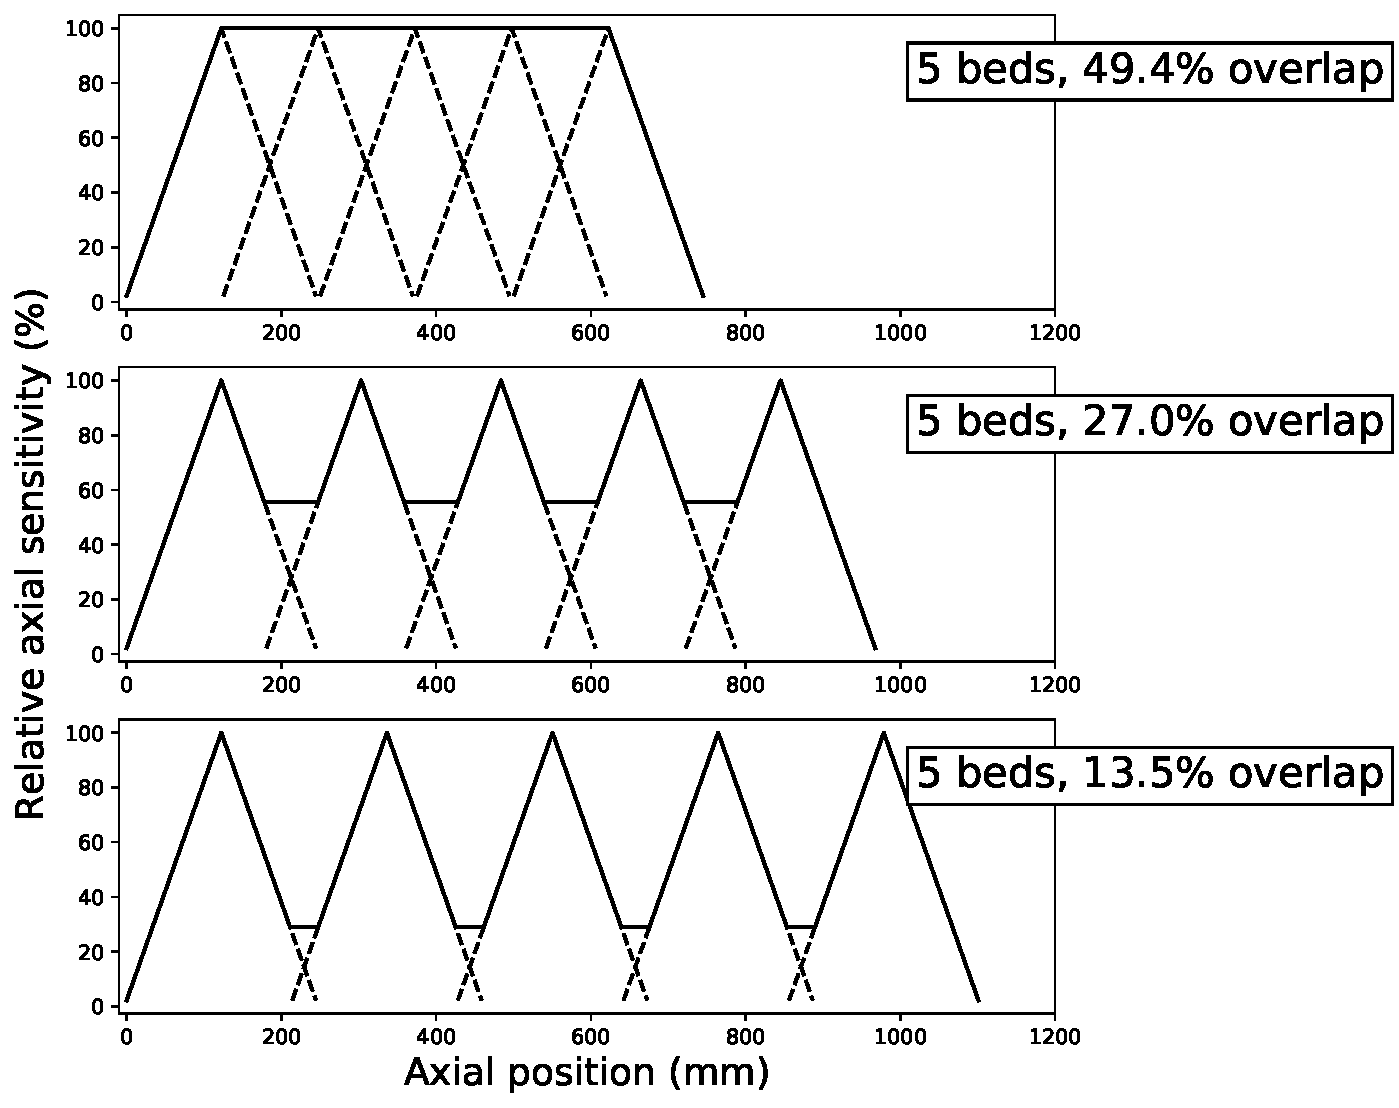
\includegraphics[scale=0.5,angle=0]{2_Theory_Methods/figures/SensitivityProfiles_3Options.pdf}
\caption{Relative axial sensitivity of 5 bed positions with decreasing overlap for the Signa PET/MR.} 
%TODO: Add over-scan in the CBM D-WB protocols. 
\label{fig3_1:decreasingOverlap}
\end{figure}
%
%
\begin{figure} [ht!]
\centering
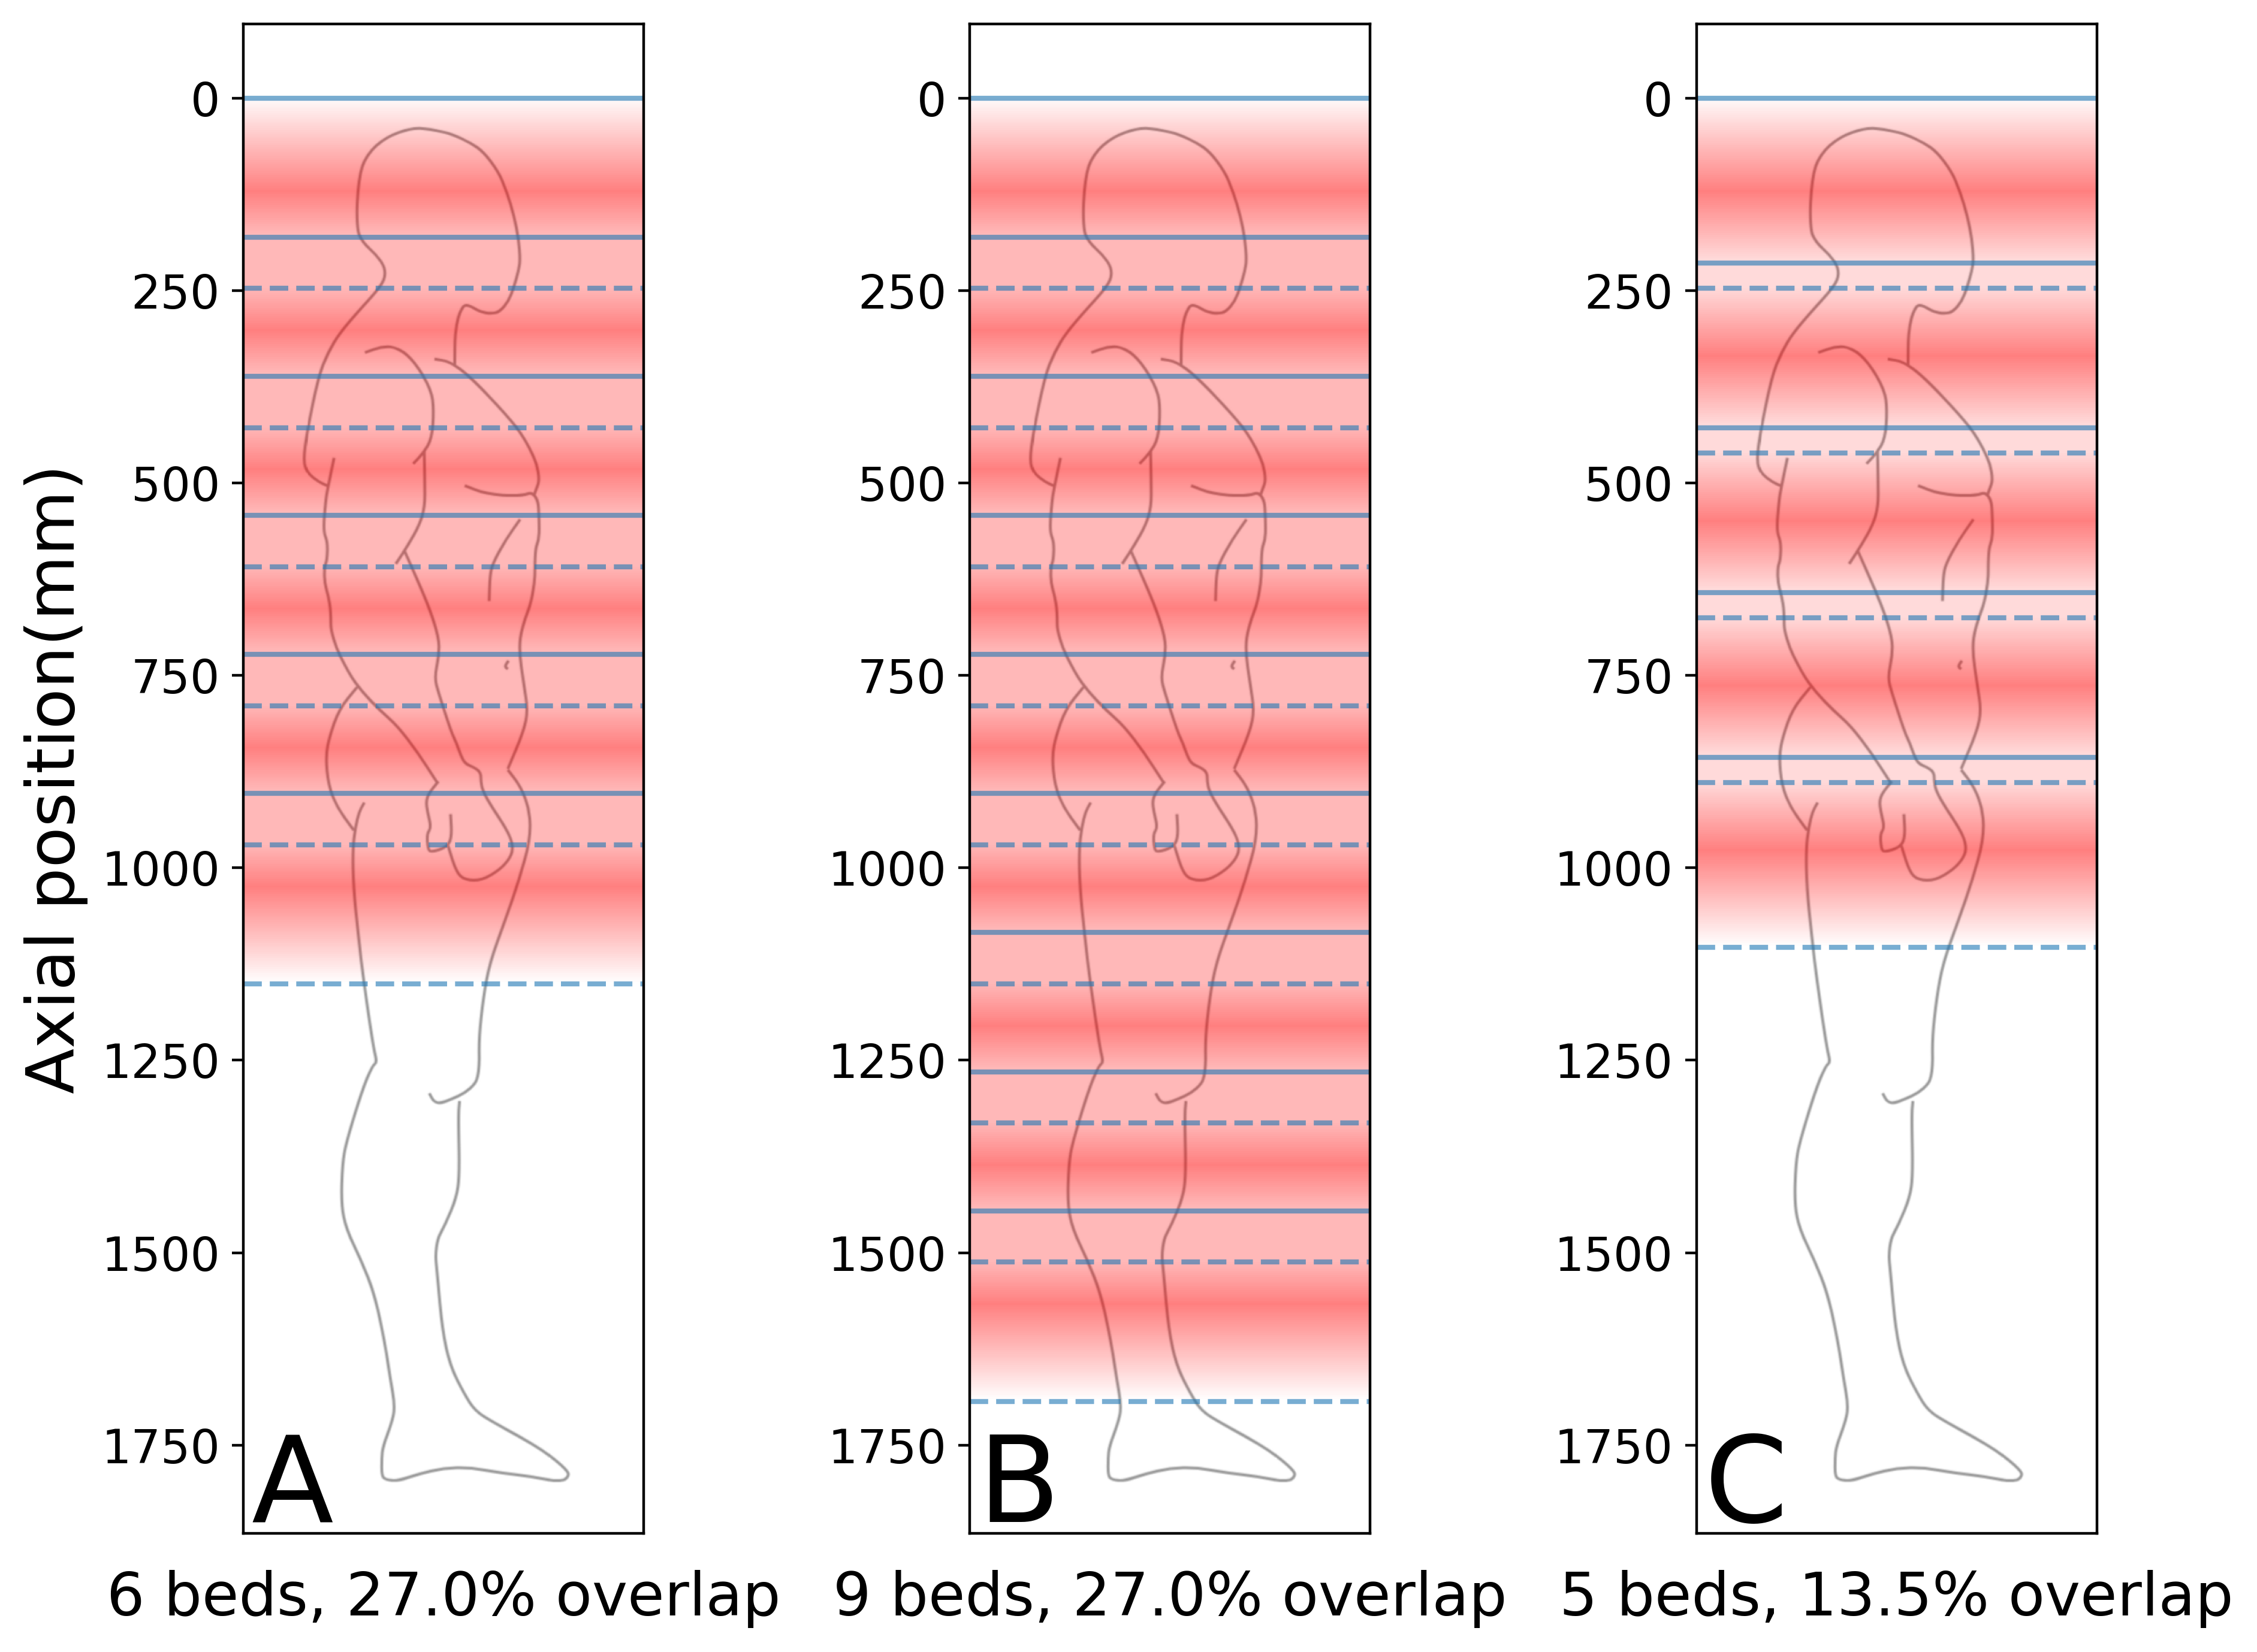
\includegraphics[scale=0.5,angle=0]{3_Results/3_1_DWB_Optimization/figures/SensitivityProfiles_overHuman.png}
\caption{Combinations of overlap and number of beds for static (A\&B) and dynamic whole-body imaging(C). Relative axial sensitivity is shown in shades of red, with bed start (\protect\tikz[baseline]{\protect\draw[line width=0.5mm] (0,.8ex)--++(1,0) ;}) and end (\protect\tikz[baseline]{\protect\draw[line width=0.5mm,densely dashed] (0,.8ex)--++(1,0) ;}) positions.} 
%TODO: Add over-scan in the CBM D-WB protocols. 
\label{fig3_1:BodyCoverage}
\end{figure}
%
%
%
\subsection{Continuous Bed Motion}
Continuous Bed Motion was proposed as an extension of step and shoot acquisition performed with small steps, to provide uniform axial sensitivity profiles~\cite{Dahlbom2001,Brasse2002}. In clinical CBM acquisition protocols the bed positional information are stored in list-mode during the examination and the data are sorted after or during the examination in histograms or sinograms (refereed as "chuncks") before reconstruction. The velocity of the bed movement can be adjusted depending on the amount of desired collected statistics, similar to the acquisition time per bed in SS acquisitions. With recent systems the bed velocity can also be varied within an examination according to the needs and distribution of the imaged activity~\cite{Panin2014}. Beyond the potential technical gains, CBM protocols have also been shown to aid in patient comfort during examination~\cite{Schatka2016}. 
%In particular for dynamic whole-body imaging many aspects of CBM acquisition can be beneficial over SS imaging~\cite{Karakatsanis2016a}.  
%
\section{Whole Body PET: Dynamic Imaging}
As outlined in the introduction, clinical and research applications can benefit from dynamic whole-body (DWB) PET information. In clinical applications DWB data can be used to construct fully quantitative parametric images for diagnosis and response monitoring of disease and pathology over the whole body. In research DWB information can enable studying of the whole body organism and interactions between different tissues, organs or compartments. 

Although recent advancements in PET have led to development of PET/CT systems with increased A-FOV, with approximately half~\cite{Karp2020,Siegel2020} or even total-body axial coverage~\cite{Cherry2018}, the majority of clinical PET systems in use are limited in the range from 15 to 26 cm~\cite{Vandenberghe2020}. 
Based on the same principles and methods used in static WB PET imaging, DWB protocols have been developed with use of repeating whole-body passes (often refereed as "sweeps"). 
These protocols can be implemented using SS acquisition, as proposed in the original work on multi-bed DWB protocols by Karakatsanis~\textit{et al.}~\cite{Karakatsanis2011,Karakatsanis2013}, or as later proposed using CBM~\cite{Karakatsanis2016a,Hu2020}. Such protocols are nowadays implemented in commercial PET/CT systems~\cite{Hu2020} and it has been shown that their use in clinical practice is feasible~\cite{Fahrni2019,Dias2020}.  Their uses in clinical imaging is an ongoing active area of research.% and yet to be proven. 
%\subsection{Challenges in multi-bed DWB protocols}
%DWB studies, similarly to single-bed single-organ dynamic studies, are limited to a total duration of one hour, for practical and patient comfort reasons. 

The transition from single-bed to multi-bed dynamic acquisition poses some considerable limitations in acquisition counts and sampling frequency. The immediate effect of the transition is the introduction of temporal gaps in the acquired data of any given bed position. These are introduced at each bed position by the time spent on imaging other bed positions and by scanner system delays due to the time required to move the bed to the next position and prepare for the next acquisition. These gaps cause a significant reduction in the sensitivity of the acquisition, with fewer total counts collected for each axial location when compared to single bed dynamic acquisitions. Furthermore, estimation of fast temporal changes in tracer uptake are compromised as the early time points of the acquisition are not fully sampled for all beds. Finally the established clinical protocols that make use of image derived input function (IDIF) to ease integration in clinical practice further sacrifice imaging time in the study’s early phase, which is spent in acquiring fast frames over a single bed location, during a dynamic single-bed (SBD) phase, centred over the heart and the aorta~\cite{Karakatsanis2013,Hu2020}.
These limitations pose considerable problems on consequent parameter estimation and in greater extend in parametric imaging performed using data from these protocols over the whole-body. These issues are addressed further in \textbf{Part \RNum{2}} of this thesis manuscript.
%
%For research applications the input function is often measured with invasive methods via an arterial catheter. In these cases the use of the initial dynamic single-bed  (SBD) phase is optional. But when estimation of pharmacokinetic parameters of interest that are sensitive to early kinetics after inject is needed, the single-bed dynamic phase can be included to estimate those parameters over a region of interest covered by the single-bed AFOV. Such use of the single-bed dynamic phase in clinical studies has also been recently explored for estimation of micro-parameters and their potential clinical applications~\cite{Zaker2020}.
%
%Typically all bed positions of the DWB mutli-bed acquisition are sampled equally with the same number of frames and so the number of WB sweeps within the DWB examination will depend on the number of frames per bed and vise versa. The number of frames that can be fitted within the study duration is limited by the system delay times, during which no data are acquired. As the characteristics of the system delays will vary for different imaging systems, it is expected that the framing will have to be adjusted for different systems too. Furthermore the expectation of the underlying kinetics, the expected tracer distribution and also the injected activity and half-life of the used radioisotope are factors that will have to be taken under consideration when considering the DWB protocol framing. 
%An optimization methodology for such parameters is outlined by Karakatsanis \textit{et al.}~\cite{Karakatsanis2013}, used in their work conducted for the characteristics of the GE Discovery RX PET/CT scanner for FDG and Patlak imaging. 

\section{Advancements on extended A-FOV PET systems}
Longer axial coverage has been a desirable characteristic for PET imaging systems, but limitations in technology and costs made it possible only during the recent years. 
As described in recent review articles, earlier attempts to make scanners beyond the 15-26 cm of \gls{afov} were successfully but at the time only for prototypes and limited by cost and hardware capabilities~\cite{Vandenberghe2020,Surti2020}.
Recently the EXPLORER consortium led to the development of scanners with 70 cm and 194 cm \gls{afov}~\cite{Karp2020,Cherry2017}. The adopted term for scanners that can encompass the whole-body is \textit{Total-body} (TP) PET, although the term is used in literature for scanner with less coverage also. More recently, a 106cm \gls{afov} PET-CT scanner was made commercially available by Siemens~\cite{Siegel2020}. 

The increase in~\gls{afov} offers many potential benefits for clinical and research applications. 
Many of the direct clinical applications of such systems are envisioned for standard of care imaging using considerably lesser injected activity, improved image quality and detection limits of lesions, faster throughput etc. Early imaging applications have shown considerable potential towards these aspirations~\cite{Badawi2019,Pantel2020}.
Beyond standard of care, many research opportunities arise from the availability of high sensitivity combined with synchronous imaging of the whole body. 
Particular for dynamic imaging over the whole-body early applications have shown feasibility of whole-body parametric imaging~\cite{Zhang2020a,Zhang2020b,Wang208}, study of fast kinetics including joint estimations of input function~\cite{Feng2019,Feng2021} as well as whole-body parametric imaging with much lesser injected activity~\cite{Liu2021}.
More details on potential uses of systems with extended~\gls{afov} are discussed further in the discussion sections and the conclusion of this manuscript.
 

\chapter{Pharmacokinetics}
\label{Chap2_2:Pharmacokinetics}
%% Brief introduction with 
\Gls{pet} is a quantitative imaging technique that makes use of 
positron-emitting radionuclides for the study of biochemical and physiological processes \textit{in vivo}. The molecules of interest for the processes under study are labelled with a radionuclide and then introduced in the body. The PET imaging system provides information about the distribution of the labelled molecules \textit{in vivo} over time and can be used to deduce information about the underlying process kinetics. 

\section{Principles of pharmacokinetic modelling}
Pharmacokinetics refers to the study of absorption, distribution, metabolism and excretion of drugs in living systems. The study of pharmacokinetics is based on measurements of concentration of drugs and their metabolites in tissues over time. Pharmacokinetic models are mathematical relationships, derived from prior knowledge or previous observations, which can be tested against the measurements in order to describe the underlying behaviour. These models describe the transport and binding rates of tracer from local concentration differences across boundaries, that can be either physical (such as a membrane or an organ outline) or conceptual boundaries as for example for example between bound and unbound tracer. These boundaries define separate compartments with distinct activity concentration which form the basis of pharmacokinetic models, also referred to as compartmental models.
%There are three assumptions are made for compartmental modelling to be valid:
%The first is the tracer assumption which requires that the presence of the tracer in PET studies is not influencing the physiological processes and molecular interactions. This is the case in most PET studies as the specific activity of the tracer (Activity/tracer concentration) is kept low. The second assumption is that the physiological processes and molecular interactions are in constant state during the duration of the PET study. The third and final assumption is that tracer is homogeneously distributed within each compartment. 

The three key assumptions underlying compartmental modelling are:
\begin{itemize}
\item The concentration of the PET tracer is not high enough to influence the physiological processes and endogenous molecular interactions under study.
\item That all physiological processes and interactions are in constant state for the duration of the PET study.
\item The assumption that tracer concentration is instantly uniform in all compartments of the model.
\end{itemize}

By common convention in pharmacokinetic modelling, the first compartment is the arterial plasma pool from where the tracer distributes to tissues. The concentration of tracer in the arterial plasma $C_P(t)$ over time $t$ is measured or deduced from population studies and applied to the model, as an input function that powers the system.
If the tracer is metabolised during the study, this process needs to be modelled using metabolite measurements. Only the concentration of parent tracer can be used as input function in quantitative analysis of the tracer kinetics.
By convention in dynamic PET studies conducted under a single session, the time point $t_0=0$ is set to be the tracer injection time. \\
Compartmental models behave according to a set of first-order ordinary differential equations, which means that change of concentration in one compartment is a linear function of the concentrations of all compartments. This linearity establishes that the measured tissue activity concentration will be the convolution of the input function with the impulse response function (IRF) of the system, which is described by the compartmental model and its parameters.
As such the tissue activity concentration $C_T(t)$ can be modelled as
\begin{equation}
 C_T(t) = C_P(t) \ast \textrm{IRF}(t)  \\ , \\ 
\end{equation}
where $\ast$ is the convolution operator. 

When a measurement of activity concentration is made with \gls{pet}, the measurement will include the underlying tissue activity and activity from the intravascular blood in this tissue. The proportion of tissue volume occupied by intravascular blood is $V_B$ is commonly referred to as blood fraction.The measured activity concentration $C_{PET}$ can be expressed as
\begin{equation}
{C_{PET}}(t)  = (1-V_{B}){C_{T}}(t) + V_{B}C_{B}(t) \\ , \\
\label{eqn:CPET}
\end{equation}
where $C_{B}$ is the total blood activity concentration.
Measurements of the %metabolite corrected
arterial plasma to total blood ratio can be made to relate between $C_{B}$ and $C_P(t)$. 
For the tracers of interest in this PhD project, the ratio of the two concentrations is stable and the relationship between the two concentrations is assumed to be $C_{B}(t) = r C_{P}(t)$. 

\section{One-tissue compartment model}
As the simplest model, the one-tissue compartment model (1TCM) can be described using two constant rates for the input and output of tracer from the tissue, $K_1$ and $k_2$ respectively. A representation can bee seen in figure~\ref{fig:1_2TCM}.

\begin{figure}[ht]
	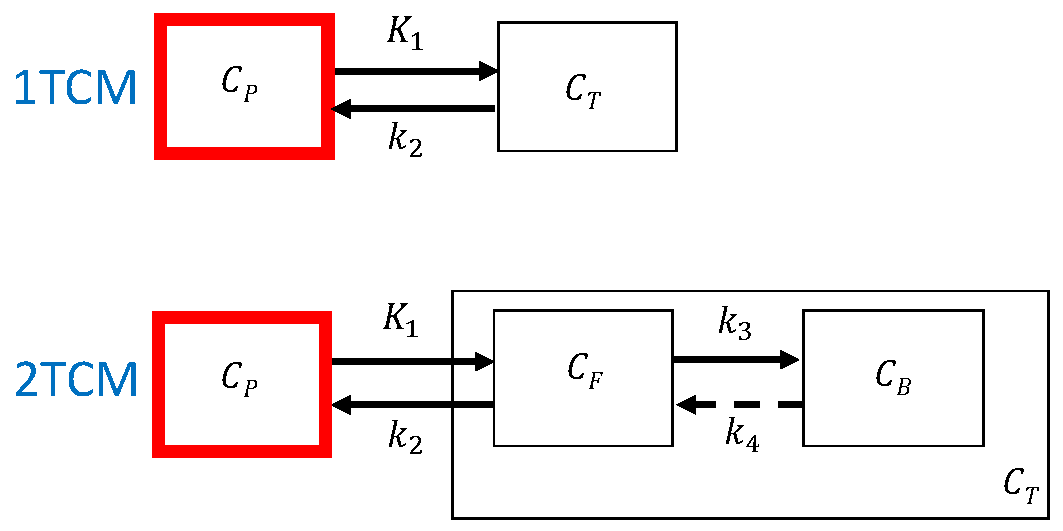
\includegraphics[width=0.8\textwidth]{2_Theory_Methods/figures/TissueCompartmentModels.pdf}
	\centering
	\caption{Representation of compartments and exchanges rates for 1TCM (top) and 2TCM (bottom)}
	\centering
	\label{fig:1_2TCM}
\end{figure}

The rate of change of the activity concentration in tissue $C_T$ will depend on the metabolite corrected arterial plasma input function $C_P$ and the activity concentration in tissue, described by the differential equation~\ref{eqn:1TCM_Diff}.

\begin{equation}
  \frac{\mathrm d C_T(t)}{\mathrm d t} = K_1 C_P(t) - k_2 C_T(t)
  \label{eqn:1TCM_Diff}
\end{equation}
\begin{equation}
   C_T = K_1 e^{-k_2 t} \ast C_P(t) 
  \label{eqn:1TCM}
\end{equation}
\begin{equation}
   C_{PET} =   K_1 e^{-k_2 t} \ast C_P(t) (1-V_B) + C_B(t) V_B
  \label{eqn:1TCM_CPET}
\end{equation}

Equation \ref{eqn:1TCM} is the solution of the differential equation \ref{eqn:1TCM_Diff}, which becomes \ref{eqn:1TCM_CPET} for the PET measurement which includes the fractional blood volume. %In equation \ref{eqn:1TCM_CPET} it is important to note that the blood fraction is related to the whole blood activity concentration $C_B$ , rather than the metabolite corrected activity concentration $C_A$. When the tracer metabolic activity is negligible and under the assumption of negligible tracer delay and diffusion from arterial to venous blood TACs, the two concentrations ($C_A = C_B$) can be set equal in favour if simplified models and estimations. 

\section{Two-tissue compartment model}
The two-tissue compartment model (2TCM) is a commonly used model as it describes the behaviour of ${}^{18}F$-Fluorodeoxyglucose (${}^{18}\mathrm{F}$-FDG), which is commonly used tracer in clinical and research PET protocols. The separation into two tissue compartments is made to distinguish between free and trapped (bound) tracer, represented as $C_F(t)$ and $C_B(t)$ respectively, with the trapping caused by the tracer being metabolised in the cells by mitochondria. The set of differential equations describing the 2TCM is shown in equations~\ref{eqn:2TCM_Diff}.

\begin{subequations}
\begin{align}
%C_{PET} = (C_F + C_B)(1-V_B) + V_B C_A \\
\frac{d}{dt}C_F(t) = K_1 C_A(t) - (k_2 + k_3)C_F(t) + k_4 C_B(t) \\ 
\frac{d}{dt}C_B(t) = k_3 C_F(t) - k_4 C_B(t)  
\end{align}
\label{eqn:2TCM_Diff}
\end{subequations}

The pathway of tracer from the trapped to the free state, via the process of dephosphorylation, is commonly considered negligible for the duration of common PET studies. With the assumption of $k_4=0$ the two differential equations in \ref{eqn:2TCM_Diff} simplify to the system \ref{eqn:2TCM_Diff_k4=0} which when solved results to equation \ref{eqn:2TCM}. 

\begin{subequations}
\begin{align}
\frac{d}{dt}C_F(t) = K_1 C_A(t) - (k_2 + k_3)C_F(t) \\ 
\frac{d}{dt}C_B(t) = k_3 C_F(t)  
\end{align}
\label{eqn:2TCM_Diff_k4=0}
\end{subequations}
%
\begin{equation}
C_T(t) =  C_F(t) + C_B(t) = K_1 ( e^{-(k_2+k_3)t} + \frac{k_3}{k_2+k_3}(1-e^{-(k_2+k_3)t})) \ast C_P(t)   
\label{eqn:2TCM}
\end{equation}

The parameters $K_1$, $k_2$ and $k_3$, which are refereed to as micro-parameters, can be estimated by fitting equation~\ref{eqn:2TCM} on measured \gls{tac} data. 

A parameter of interest for clinical studies, is the influx rate constant $K_i$, given by equation~\ref{eqn:FDG_Ki}. This is considered as a macro-parameter of the system and can be understood as the the proportion of flux $K_1$ that results to trapped tracer. 

\begin{equation}
K_i = \frac{K_1 k_3}{k_2+k_3}
\label{eqn:FDG_Ki}
\end{equation}


\section{Gjedde-Patlak linearisation method}

Direction estimation of model micro-parameters, such as those of~\ref{eqn:2TCM}, requires non-linear fitting optimization procedures. These are commonly time consuming and their estimations are susceptible to noise.
For parametric imaging, where the model estimation has to be performed for every voxel of the image, estimation of micro-parameters is commonly avoided due to the poor statics and high noise associated with \gls{tac} measurements at the voxel level. 
Linearisation methods allow for transformation of the measured data, to enable use of linear least-square fitting procedures for estimation of model macro-parameters, under certain assumptions. Furthermore these methods reduce the number of parameters to be estimated, thus reducing the variability of estimates and sensitivity to noise. 

With the assumption of irreversible tracer behaviour the Gjedde-Patlak method has been developed, described by Gjedde~\cite{Gjedde1982} and Patlak \textit{et al.}~\cite{Patlak1985}. The proposed transformation is

\begin{equation}
\label{eqn:PatlakModel}
\frac{C_{T}(t)}{C_{P}(t)} = K_i \frac{\int_{0}^{t} C_{P}(\tau) d\tau}{ C_{P}(t)} + V_{\alpha}   \ , \;  t>t_{ss} \ ,
\end{equation}

where $K_i$ is the steady state trapping rate and $V_{\alpha}$ the apparent volume of distribution. The transformation is valid for time points $t$ after steady state conditions are achieved at time $t_{ss}$. Steady state conditions are achieved when the reversible compartments are in steady-state equilibrium with the plasma blood compartment. 

The Gjedde-Patlak linearisation method, refereed simpler as \textit{Patlak model}, is commonly used with the 2TCM model for FDG, under the assumption of $k_4=0$. In this case the Patlak model parameters can be related to micro-parameters using equation~\ref{eqn:FDG_Ki} and 

\begin{equation} 
V_a  = \frac{K_1 k_2}{(k_2+k_3)^2} \\ . \\ 
\end{equation}

%For a PET measurement the observed activity $C_{PET}(t)$ described by equation~\ref{eqn:CPET}.
With the assumption of $C_{B}(t) = r C_{P}(t)$, we can substitute equation~\ref{eqn:PatlakModel} into equation~\ref{eqn:CPET} and describe the observed activity $C_{PET}(t)$ using the Patlak model as

\begin{equation} 
{C_{PET}}(t)  = \underbrace{(1-V_{B})K_i}_{\theta_1} \int_{0}^{t} C_{P}(\tau) d\tau +  \underbrace{V_{\alpha}+r V_{B}}_{\theta_2} C_{P}(t) \\ , \\
\label{eqn:PatlakCPET}
\end{equation}

where the Patlak slope $\theta_1$ and the Patlak intercept $\theta_2$ are the model parameters that can be estimated from TAC measurements of ${C_{PET}}(t)$. 

%It is important to note a limitation of the Patlak model, which  that the estimated $K_i$ from the Patlak slope $\theta_1$ is susceptible to systematic errors in its estimation and can deviate from the true underlying $K_i (= \frac{K_1 k_3}{k_2+k_3})$.
A limitation in the use of the Patlak model using equation~\ref{eqn:PatlakCPET} is that $V_B$ is not necessarily known a priori and Patlak analysis can not distinguish between $K_i$ and $(1-V_B)$. In many applications $V_B$ is assumed to be small ($\leq$0.05) and neglected, but it can be a cause for systematic errors. 
In the applications of the Patlak model in this project, we will refer to the slope $\theta_1$ as the Patlak $K_i$ value, which is the value of interest that is commonly used in practice with Patlak analysis.


\section{Spectral analysis method}
The Spectral analysis method was originally introduced by Cunningham et al. \cite{Cunningham1993}. The method is based on the general form of the solutions of compartmental models and describe the generic behaviour of any compartmental system as a weighted positive sum of decaying exponential functions with decay rates $\beta$ which describe the exchange between compartments, convolved with an input function. 

The spectral analysis model for $C_T(t)$ can be expressed using M functions as

\begin{equation} 
\label{eqn:SpectralModel}
C_{T}(t)  =  \sum_{b=0}^{M-1} {\phi_b}  e^{-\beta_b t} \ast C_P(t)   \\ , \\
\end{equation}

where $\phi_b$ are the model coefficients (constrained to positive values) for the exponential functions with decay rates $\beta_b$ that describe the exchange between compartments. 

The advantage of this methodology is that it can be used to fit on \gls{tac} data, with no prior knowledge and assumptions on the underlying kinetics. Additionally, it can be used to deduce information of the underlying kinetics using the basis pursuit strategy proposed by Gunn \textit{et al.}~\cite{Gunn2002}.
Macro-parameters of the underlying model can also be deduced using the spectral analysis fitted model. Tracer delivery to tissue $K_1$ can be estimated directly with
\begin{equation} 
\label{eqn:SpectralModel_K1}
K_1  =  \sum_{b=0}^{M-1} {\phi_b}   \\ . \\
\end{equation}

For reversible kinetics, the parameters can be used to deduce the volume of distribution $V_D$ as
\begin{equation} 
\label{eqn:SpectralModel_VD}
V_D  =  \sum_{b=0}^{M-1} \frac{\phi_b}{\beta_b}   \\ . \\
\end{equation}

For irreversible kinetics, an parameter is used in the model to account for the trapping rate $K_i$. In this work we use parameter ${\phi_0}$ to describe irreversible trapping, with its respective exponential decay rate set to zero ${\beta_0} = 0 $. With this assumption the model becomes

\begin{equation} 
\label{eqn:SpectralModel_VD}
C_{T}(t)  =  \sum_{b=0}^{M-1} {\phi_b}  e^{-\beta_b t} \ast C_P(t)  =  \phi_0 \ast C_P(t) + \sum_{b=1}^{M-1} {\phi_b}  e^{-\beta_b t} \ast C_P(t)  \\ , \\
\end{equation}

for which $K_i = {\phi_0}$. 

Finally, to model the observed activity $C_{PET}(t)$ using the spectral analysis model, we can substitute equation~\ref{eqn:SpectralModel} into equation~\ref{eqn:CPET} and assume again that $C_{B}(t) = r C_{P}(t)$ to get

\begin{equation} 
{C_{PET}}(t)  = (1-V_{B}) \sum_{b=0}^{M-1} {\phi_b}  e^{-\beta_b t} \ast C_P(t) + V_{B} r C_P(t)   \\ . \\
\label{eqn:SpectralCPET}
\end{equation}

If we account for the parameter $(1-V_{B})$ into the weights $\phi_b$, the equation can be written in short as 

\begin{equation} 
{C_{PET}}(t)  = \sum_{b=0}^{M} {\phi_b} e^{-\beta_b t} \ast C_P(t)   \\ , \\
\label{eqn:SpectralCPET_short}
\end{equation}

for which $\beta_b \xrightarrow[]{}\inf$ and $\phi_M = r V_{B}$. 
When fitted on measured ${C_{PET}}(t)$ data , the spectral model in equation~\ref{eqn:SpectralCPET_short} can be used to deduce $K_1$ and either $V_D$ or $K_i$ using

\begin{subequations}
\label{eqn:AllSpectralEqns}
\begin{align}
K_1 = \frac{\sum_{b=0}^{M-1} {\phi_b}}{1-{\phi_M}}   \\  
V_D = \sum_{b=0}^{M-1} \frac {\phi_b}{\beta_b (1-\phi_M)} \\
K_i = \frac{\phi_0}{1-\phi_M} . 
\end{align}
\label{eqn:SpectralCPET_AllEquations}
\end{subequations}

\subsection{Choice of spectral rates}

On equation~\ref{eqn:SpectralCPET_short} the spectral rates $\beta_1 ... \beta_{M-1}$ are used to describe the exchange between compartments. These are set to cover the range of expected underlying kinetics and are commonly logarithmically spaced within that range~\cite{Gunn2002}.
As a rule of thumb, the lower limit of the range can be set to $\beta_1 = 1/(3 T_{end})$ where $T_{end}$ is the total time of the PET study, and the upper limit of the range can be set to $\beta_{M-1} = 3/T_{in}$ where $T_{in}$ is the duration of the first frame of the study~\cite{Veronese2016}.

In spectral analysis the size of the spectral parameters used is empirically set in the 10$^2$ order of magnitude. This relatively large number allows for clear separation of the underlying exchange rates, for deduction of models of the underling behaviour. 
For use with dynamic reconstruction, as described in the following chapter, a smaller number of parameters is used that is adequate to model the PET measurements and reduce the numbers of parameters to estimate and the noise on result parameter estimates. 

\section{IsotoPK pharmacokinetic study}

Traditionally it has been assumed that passive diffusion is the main mechanism that controls drug delivery to tissues. 
But more recently, it is recognised that the presence of membrane transporters at blood-tissue interfaces suggests that transporters play an important role in drug pharmacokinetics. Imaging studies can play an important role in the study of their distribution and function in regards to drug delivery to tissues over the body~\cite{Marie2017}. \\

To this purpose, a novel PET tracer has been developed using Glyburide (glibenclamide, GLB) and $^{11}$C, targeting many transporters of the Solute Carrier O (SLCO) family~\cite{Tournier2013,Caille2020}. Preliminary studies have indicated that these transporters are expressed mainly in the liver and the kidneys~\cite{Tournier2013}.

A first in man study, named \textit{IsotoPK}, was designed and conducted for the study of the distribution of these transporters in healthy volunteers~\cite{Marie2019}.
The study was conducted on the Signa PET/MR, using a Dynamic Whole Body (DWB) acquisition protocol, with two acquisitions per volunteer to study the distribution without and with the administration of an inhibitor substance prior to PET imaging.
Arterial blood samples for deduction of an input function and metabolite analysis we collected manually during the duration of each scan. 

Initial results on three volunteers have shown that Glyburide is very slowly metabolised and did not require to be accounted for in PET analysis, as their impact on PET quantification would me minimal. They also showed strong binding with plasma ($\geq$ 90\%).
Predominant uptake of the tracer was seen in the liver and also the kidneys. Lower uptake was observed in the spleen, the aorta wall and the pancreas. At all other tissues no strong signal was seen.  

\section{PET analysis in the liver}
\label{liver_PV_theory}
One of the unique characteristics of the liver, in regards to pharmacokinetic modeling, is that it is supplied with blood via two routes. The hepatic artery (HA) accounts for approximately 25\% of the blood supply in the liver, while the portal vein (PV) accounts for the rest 75\%. The portal vein delivers blood that has been filtered mainly by the gastrointestinal tract, a process which alters the characteristics of the input function associated with portal vein in relation to the arterial input function. 

Studies on pigs and non-invasive studies on humans have produced methods to model the PV input function as a dispersion of the arterial input function~\cite{Kudomi2008,Winterdahl2011}, which can be modelled using 

\begin{equation} 
{C_{PV}}(t)  = {k_g} e^{-k_g t} \ast C_P(t)   \\ . \\
\label{eqn:PortalVein}
\end{equation}

With knowledge of the $k_g$ dispersion value and ratio between PV and HA input, the liver input function ${C_{H}}(t)$ can be then modelled as

\begin{equation} 
{C_{H}}(t)  = 0.75 \cdot C_{PV}(t) + 0.25 \cdot C_{P}(t)  \\ . \\
\label{eqn:HepaticInput}
\end{equation}

An example demonstration of the two components of ${C_{H}}(t)$ is shown in figure~\ref{fig_2_2:LiverDualInputFunction}.

\begin{figure} [h!]
\centering
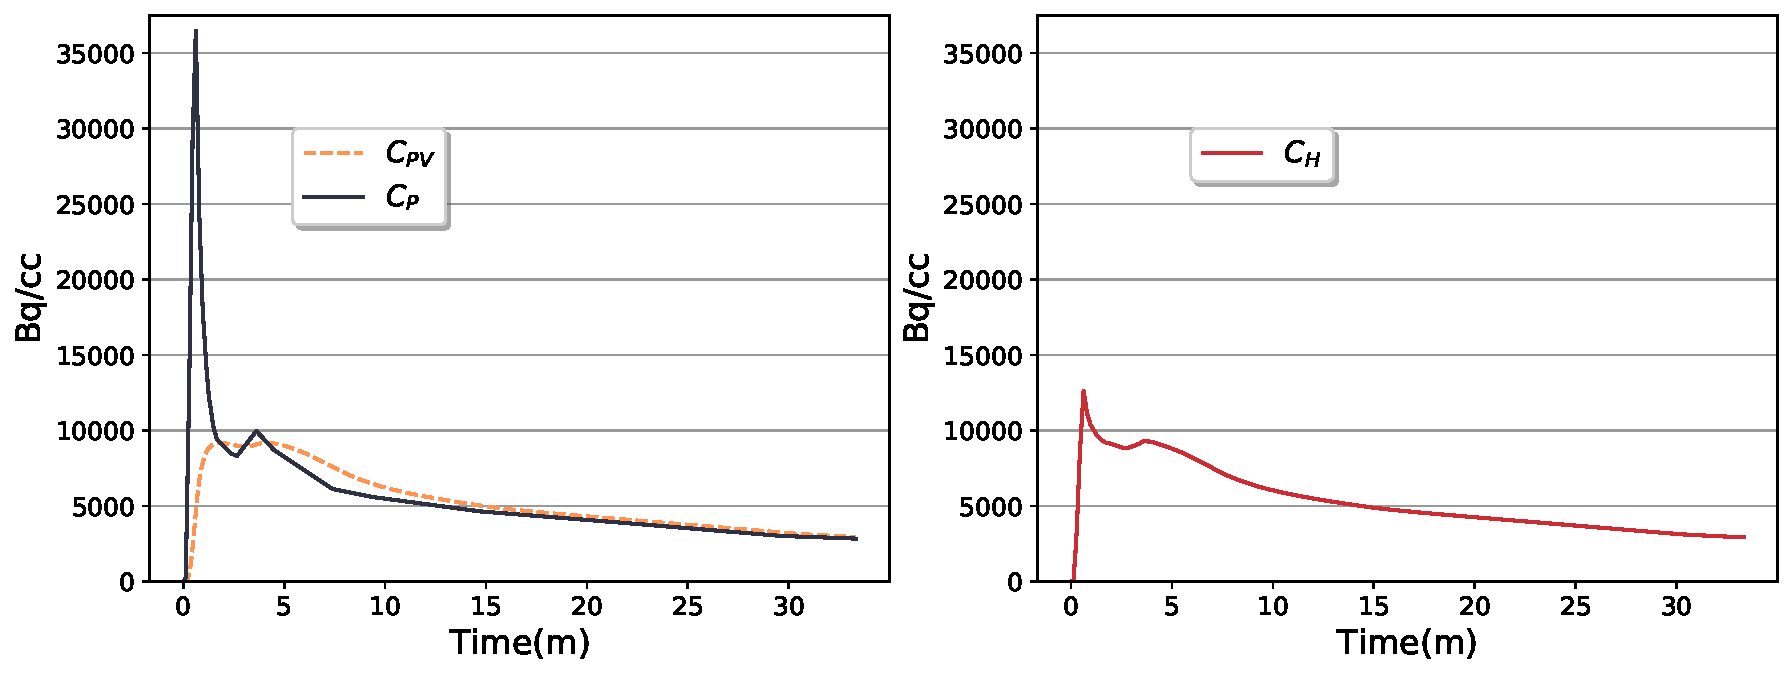
\includegraphics[scale=0.53,angle=0]{2_Theory_Methods/figures/2_2_LiverDualInputFunction.pdf}
\caption{Example arterial input function $C_{P}(t)$ and modelled PV input function (using $k_g$=0.5 min$^{-1}$~\cite{Kudomi2008}) (left). Combination of arterial and PV input function to provide ${C_{H}}(t)$, assuming a 25/75 ratio (right).} 
\label{fig_2_2:LiverDualInputFunction}
\end{figure} 

Use of imaging information for non-invasive estimation of the portal vein input function and their effects in pharmacokinetic model estimates over the liver are an active area of research~\cite{Wang2018,HernandezLozano2019} with no standardised and widely accepted practices.

%\subsection{Tracer redistribution}
%Another aspect 



\chapter{Reconstruction}
\label{Chap2_3:Reconstruction}
%Image reconstruction is necessary to produce images of activity distribution from the acquired tomographic measurements. Reconstruction algorithms used for this process can be categorised as either analytical or statistical reconstruction methods.  
Analytical reconstruction methods seek to invert the transformation that links the image to data domain, using linear analytic approaches. These methods treat the measured LOR data as line integrals over image space and necessitate corrections to be applied on projection data prior to reconstruction, in order to result to valid and quantitatively accurate images. Traditionally the most commonly used analytical reconstruction method is \textit{Filtered Back Projection} which is described very briefly in this chapter. 
Statistical reconstruction methods are derived from statistical formulations of the detection process and allow for the use of complex system models that include various effects of the acquisition process. These methods result in non-linear formulations of the reconstruction problem which require iterative optimisation methods to reach a solution. The solution sought is a set of image parameters (that describe the activity distribution) which best describes the acquired tomographic data. 
In this thesis project we made exclusive use of statistical reconstruction methods due to their ability to incorporate complex system models, including dynamic models which was crucial for the aims of this thesis.

\section{Projection and back-projection process}
Coincidence detection of annihilation photons in PET leads naturally to a line-integral model where the number of coincidence events of an \gls{lor} is approximately linearly proportional to the integral of tracer density along the volume joining the two detectors. 
The projection process can be written as
\begin{equation}
   \bm y = proj\{\bm{\lambda}\}  \\, 
  \label{eqn:Radon}
\end{equation}
where $\bm{\lambda}$ is the continuous distribution of radiotracer and $\bm{y}$ the continuous projection data (or else sinogram data).
The 2D projection operation is also known as the Radon transform~\cite{radon1917,Radon1986} and translates from the image to the projection data domain. Projections in 3D can be made using the X-ray transform or extension of the Radon transform~\cite{Natterer1986}. 
The projection's dual operation is back-projection, which translates from the data domain to image domain.
%
\subsection{Image representation}
In practice the spatio-temporal radiotracer distribution is described using a model with a finite number of parameters. The most common choice in common practice is the use of equally sized non-overlapping voxels that cover the useful \gls{fov}. Their use can also extend to the temporal domain with a set of voxels describing the \gls{fov} for each temporal bin. In this case the sets of voxels per temporal bin are considered temporally independent.
If for a moment we consider only the spatial domain and static imaging, we can model the spatial radiotracer distribution $\bm{\lambda}$ using voxels with the  $rect$ function as
\begin{equation}
   g(\bm{r};\bm\lambda) = \sum_{j=1}^{n_{j}} \lambda_j {rect}(\bm{r}-\bm{r}_j)  \\, 
\end{equation}
for an ${n_{j}}$ number of voxels with $r_j$ coordinates and intensity $\lambda_j$.
For the linear model case, the set of functions describing the distribution are referred to as \textit{spatial basis functions}. From here on we will be using the $\bm\lambda$ symbol to refer to the ${n_{j}}$ dimension vector of $\lambda_j$ voxel weights that describe the spatial activity distribution as 
\begin{equation}
   \bm\lambda = \big\{ \lambda_j| j=1,\cdots,n_j \big\} \\.
\end{equation}
If we now consider the temporal domain of the activity distribution as well, the $rect$ function can be used 
on the time domain to define a set of $n_t$ independent temporal bins (frames). Later in this chapter we will show how dynamic models can be used to describe the behaviour of voxel values across the temporal domain, but traditional reconstruction treats frames as independent static detests.
In this case the activity distribution of each frame can be written as
%\begin{equation}
%   \bm{\lambda} = \Big\{ {\bm{\lambda}_m,m=1,..,n_m} \Big\} \\,
%\end{equation}
%where
\begin{equation}
   \bm{\lambda_t} = \big\{ {\lambda_{tj}| j=1,\cdots,n_j} \big\} \\.
\end{equation}
Equivalently the projection data are binned according to the discretization imposed by the \glspl{lor} in $y_i$, where $i$ is the projection bin index and $n_i$ the total number of \glspl{lor}. Similarly to the image data, the projection data are binned temporally into $y_{ti}$ for each projection bin $i$ at frame $t$ for a total number of number of $n_t$ frames. 
The data of each frame can then be written as
%\begin{equation}
%   \bm{y} = \Big\{ {\bm{y}_m,m=1,...,n_m} \Big\} \\,
%\end{equation}
%where
\begin{equation}
   \bm{y_t} = \big\{ {y_{ti}| i=1,\cdots,n_i} \big\} \\.
\end{equation}
%
\subsection{Projection \& Analytical reconstruction}
Forward projection of image to data space can be treated by summing contributions of voxels across each~\gls{lor}. %Different projection strategies exist that model the contribution of voxels differently depending on their placement in the \gls{lor}. 
As this is a computationally heavy process in practice, different methods have been proposed that balance between accuracy and consistency and computing requirements. %A short follows list with basic description of the methods that are implemented in CASToR.
Some of these methods, which are also implemented in the CASToR reconstruction software, are listed bellow with a short description.
\begin{itemize}
\item  \textbf{Siddon projector}~\cite{Siddon1985}: Weights the contribution of an LOR to each by the length of the line that intersects the voxel.
\item  \textbf{Distance driven}~\cite{DeMan2004}: An optimised method for calculating weights by mapping pixel boundaries and detector boundaries for each projection to a common axis .
%\item  \textbf{Incremental Siddon}~\cite{Jacobs2015}:
\item  \textbf{Joseph}~\cite{Joseph1982}: Estimates contribution of voxels to LOR based on linear interpolation and their distance from the LOR. 
\item  \textbf{Multi-Siddon}~\cite{Moehrs2008}: Uses multiple lines from the faces of the detectors in each LOR to approximate the volume intersected between the two detectors and the voxel.
\end{itemize}

%\begin{figure} [h!]
%\centering
%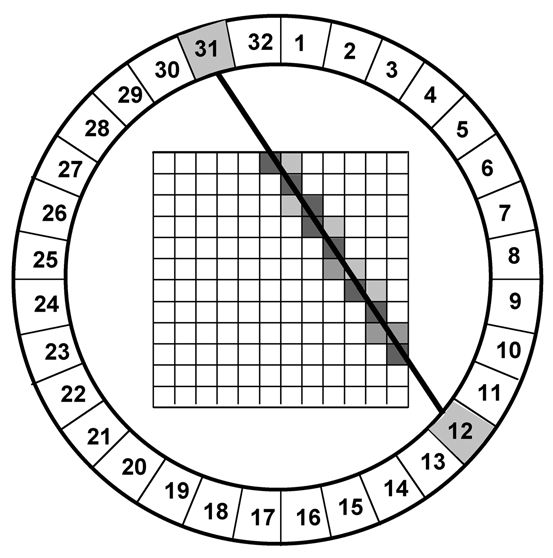
\includegraphics[scale=0.35,angle=0]{2_Theory_Methods/figures/Radon_Discrete.png}
%\caption{Back-projection of a single LOR through image space, with contribution weighted according to the length of the line that intersects the voxel.} 
%\label{fig_3:back_projection.}
%\end{figure} 
Similarly, the back-projection operation assigns to voxels in the \gls{fov} the contribution from each \gls{lor} bin, using the same methods.
Analytical reconstruction methods seek to estimate an image by inversion of the forward-projection process, by superimposing contributions from all \glspl{lor} in image space. 
This results to analytical algorithms, including the most widely used algorithm of \textit{Filtered Back Projection} (FBP).
%In practice a filtered version of the projections is back-projected to account for the non-uniform number of contributions from LORs in different regions of the image space, which gives the processes the name of filtered back projection. The method can be extended to 3D via use of the 3D X-ray transform and approximations of missing data projections~\cite{Kinahan1989}. 
But while analytical reconstructions are linear processes and computationally fast, accuracy is limited by the simplistic assumptions of the line integral model, ignoring many degrading effects such as positron range, variations in response across \glspl{lor} etc. In addition these methods do not account for the statistical properties of the detection process in the data.
Finally, the FBP algorithm seeks to solve an ill-posed problem meaning that small changes in the data can result to largely disproportional effects on the reconstructed image. As the projection data include stochastic noise from the detection process, the reconstruction results to artefacts. In practice smooth low pass filters, like the Hann apodization filter, are applied in the reconstruction process to reduce the strength of these artefacts at the cost of degraded spatial resolution. The sub-optimal trade-off between strength of artefacts and spatial resolution can be adjusted by changing the filter's cut-off frequency.

\section{Formulation of the system model}
The analytical reconstruction methods are based on the idealised description of the scanning process using the line integral model. But in reality there are many effects that should ideally be considered in the scanning system model. For example the statistical nature of the detection process, positron range and detection resolution effects, the detection of scattered and random events as well as the discrete nature of the detection and scanner geometries that do not result to complete sampling.
But as the scanning model complexity is increased, analytic expressions that seek to inverse the scanning process are not feasible.
For this reason iterative algorithms are employed, which seek a solution by optimising an objective function that expresses some difference measure between the measured data and the modelled data from an image estimate.

We can define the system model using an $n_i \times n_j$ system matrix $\bm{P}$. Each element $P_{ij}$ of the matrix is the probability of detection by voxel $j$ to data bin $i$. 
As discussed, many effects can be included in this matrix elements which will be outlined bellow. By contrast scatter effects can be hard to implement in the system matrix and random effects are non-linear effects that cannot be modelled linearly. As such the scatter and random events are considered to be known for each detector bin and included as an additive background $b_i$ for each data bin $i$ in the system model.

The model of the data at bin $i$ from an image $\bm{\lambda}$ can be written as a sum over voxels of the probability of detection in this bin 
\begin{equation}
   \hat{y_i} = \sum_{j=1}^{n_j} P_{ij} \lambda_j + b_i ,
   \label{eqn:system_model}
\end{equation}
where $\hat{y_i}$ is the modelled data or expectation of the data.

The system matrix can be decomposed to the individual contributing components as separate sparse matrices and vectors
\begin{equation}
   \hat{y_i} = n_i a_i \sum_{j=1}^{n_j} X_{ij} \sum_{k=1}^{n_j} H_{jk} \lambda_{jk} + b_i ,
\end{equation}

where
\begin{itemize}
    \item $n_i$ are the normalisation factors for each LOR bin
    \item $a_i$ are the attenuation factors for each LOR bin
    \item $X_{ij}$ is the geometrical projection matrix
    \item $H_{jk}$ is the resolution modeling matrix, applied as a convolution in image space
    \item $b_i$ the background events for each LOR bin.
\end{itemize}
%
Resolution modelling can be applied on both data and image space of the system model, but in practice is applied on one of the two domains~\cite{Stute2013}. In the CASToR reconstruction software that was used in this project, resolution modelling is implemented in image space as written in the above expression.

If \gls{tof} measurements are available, the additional information regarding the probability of the annihilation event along the \gls{lor} can be incorporated in the model. \Gls{tof} weights are assumed to be independent of the other system matrix elements, and thus act as an additional multiplication factor. Depending on the type of \gls{tof} information, the weights can either be quantized (for each \gls{tof} bin) or expressed as a continuous function. More details on both options and the implementation of \gls{tof} reconstruction can be found in the work of Filipović~\textit{et al.}~\cite{Filipovic_2019}. 
%
\section{Formulation of the objective function}
%As discussed above, iterative reconstruction relies in optimisation of an objective function. 
We can consider the total number of events in each projection bin to be modelled as a random sample from a Poisson distribution. According to the probability mass function, the conditional probability or likelihood function for $\hat{y_i}$ given the measured data ${y_i}$ will be
\begin{equation}
p({y_i}|{\hat{y_i}}) = L({\hat{y_i}}|{y_i}) = e^{-\hat{y_i}} \frac{\hat{y_i}^{y_i}}{{y_i}!}  \\  .
\end{equation}
With the assumption that measurements of counts in each bin are independent random processes, the likelihood of the data over all bins will be
\begin{equation}
p(\bm{y}|\bm{\hat{y}}) = L(\bm{\hat{y}}|\bm{y}) = \prod_i^{n_i} e^{-\hat{y_i}} \frac{\hat{y_i}^{y_i}}{{y_i}!} . 
\label{eqn:probability}
\end{equation}
By substituting the system model equation \ref{eqn:system_model} in equation~\ref{eqn:probability}, we can write an expression of likelihood of the image $\bm{\lambda}$ given the measured data $\bm{y}$.
\begin{equation}
    L(\bm{\lambda}|\bm{y})  = \prod_i^{n_i} e^{-(\sum_{j=1}^{n_j} P_{ij} \lambda_j + b_{i} )} \frac{(\sum_{j=1}^{n_j} P_{ij} \lambda_j + b_{i} )^{y_i}}{{y_i}!}
\end{equation}
This expression can be used as the objective function in the optimisation process of seeking the most likely (ML) estimate of $\bm{\lambda}$ from a measurement $\bm{y}$ . 
It is more convenient to take the expression of the log likelihood and since the log function is monotonic the log likelihood can be used to arrive to the same ML estimate.

The log likelihood expression is
\begin{equation}
    lnL(\bm{\lambda}|\bm{y})  = \sum_{i=1}^{n_i}\left[ y_i ln(\sum_{j=1}^{n_j} P_{ij} \lambda_j + b_i) -\sum_{j=1}^{n_j} P_{ij} \lambda_j - b_i - ln({y_i}!) \right] \\.
\label{eqn:log_likelihood}
\end{equation}
This expression of the Poisson log-likelihood will be used to arrive to the maximum likelihood estimate image $\bm\lambda$, which will be noted as $\bm{\lambda}^{ML}$, that maximises the likelihood of the modelled data given the measured \mbox{data $\bm{y}$}. 
\begin{equation}
\bm{\lambda}^{\textrm{ML}} = \argmax{\bm{\lambda}}(lnL(\bm{\lambda}|\bm{y}))
\end{equation}
\section{Maximum Likelihood - Expectation Maximisation}
\label{section:MLEM}
The second partial derivative of the log-likelihood to $\lambda_j$ can be shown to be negative semidefinite to all allowed images and thus the log-likelihood function is a concave function. This means that a found local maximum though the optimisation process will be the global maximum of the function.

Seeking to solve equation~\ref{eqn:log_likelihood} to find analytically the maximum likelihood image $\bm{\lambda}^{ML}$, we can take its first partial derivative to $\lambda_j$ and set it to be equal to zero. 
\begin{equation}
\frac{\partial lnL(\bm{\lambda}|\bm{y})}{\partial \lambda_j} = \sum_{i=1}^{n_i}\left[  y_i \frac{\sum_{j=1}^{n_j} P_{ij} }{\sum_{j=1}^{n_j} P_{ij} \lambda_j + b_i} -\sum_{j=1}^{n_j} P_{ij}
\right]  = 0 \\,
\end{equation}
but this expression has no closed form solution.
The arrival to this expression shows the need for iterative methods to seek the $\bm{\lambda}^{\textrm{ML}}$ solution. 

The most common algorithm used for this problem is the Expectation Maximisation algorithm that was first applied on statistical PET reconstruction by two key works by Shepp and Vardi~\cite{Vardi1985} and Lange and Carson~\cite{Lange1984}. In these works the solution is derived though the introduction of the "complete data" concept~\cite{Dempster1977}. \\
Let $\bm{z}$ be the complete data random dataset of $x_{ij} + g_i$ values which describes the exact number of emissions from voxel $j$ that contribute to the measurement at projection bin $i$, with the many to one mapping 
\mbox{$y_i = \sum_{j=1}^{n_j} x_{ij} + g_i$}.
The complete dataset is unknown, but the conditional expectation of the complete data can be expressed using an image estimate (a guess) noted as $\bm{\lambda}^{(k)}$ and the measured data $\bm{y}$ as 
%
\begin{equation}
\label{eq:Complete_Data_Expectation1}
\hat{x}_{ij}(\bm{\lambda}^{(k)},y_i) = y_i
\frac{P_{ij} \lambda_j^{(k)}}{\sum_{d=1}^{n_j} P_{id}\lambda_d^{(k)} + b_i} \\ , 
\end{equation}
%
\begin{equation}
\label{eq:Complete_Data_Expectation2}
\hat{g}_{i}(\bm{\lambda}^{(k)},y_i) = y_i 
\frac{b_i}{\sum_{d=1}^{n_j} P_{id}\lambda_d^{(k)} + b_i} . 
\end{equation}
%

The complete dataset follows a Poisson distribution, with its log-likelihood being
\begin{equation}
lnL(\bm{\lambda}|\bm{z}) = 
\sum_{i=1}^{n_i} \left[\sum_{j=1}^{n_j}( x_{ij} ln(P_{ij}\lambda_j) - P_{ij} \lambda_j) +
g_i ln(b_i) - b_i \right] \\ ,  
\label{eqn:log_likelihood_z}
\end{equation}
where parameters not related to its optimisation to $\lambda$ have been dropped. 
If we replace the expectation of the complete data using equations~\ref{eq:Complete_Data_Expectation1} and ~\ref{eq:Complete_Data_Expectation2} we can then seek to maximise this likelihood function to obtain the ML image estimate of the expected complete data. Using the Kuhn-Tucker conditions we arrive to a closed form solution
\begin{equation}
\lambda_j^{(k+1)} = \frac{\lambda_j^{(k)}}{\sum_{i=1}^{n_i} P_{ij}} 
\sum_{i=1}^{n_i} P_{ij} 
\frac{y_i}{\sum_{d=1}^{n_j} P_{id}\lambda_d^{(k)} + b_i } \\,
\label{eqn:MLEM}
\end{equation} 
that provides a new estimate $\bm{\lambda}^{(k+1)}$. This single update equation combines the two steps of the optimisation process. First, given an image estimate $\bm{\lambda}^{(k)}$ the expectation of the complete data is estimated. Then, the log-likelihood of the expectation of the complete data is maximised. This iterative process results in monotonic increase of the original log-likelihood function. This process is the \textit{MLEM} algorithm.
%Together with the expression for the conditional expectation of the complete data, the two step process of Expectation Maximisation and  Maximum likelihood estimation can be written in a single update equation. Given data $\bm{y}$ and an image estimate $\bm{\lambda}^{(k)}$ , the updated image estimate $\bm{\lambda}^{(k+1)}$ is given from:
%This equation forms a single update of the MLEM algorithm, which when evaluated over all voxels $j$ provides an updated image $\bm{\lambda}^{(k+1)}$. 

The use of the conditional expectation of the data is in fact an example of the general concept of optimisation transfer, where the construction of surrogate functions is made to be used with simpler optimisation process, that leads to optimisation of the main function as well. One advantage of this algorithm is that an update over all voxels of the image can be made with a single pass over the data. The disadvantage is that it results to very slow convergence speeds. 
To accelerate convergence the Ordered Subsets algorithm is used in most practices, which makes use of subsets of the data at each update step (each subset) to reduce computing time for each image update. 

\section{Dynamic reconstruction}
\label{section:Fully_4D_reconstruction}
Soon after the proposition of the EM algorithm for iterative PET reconstruction by Shepp and Vardi~\cite{Vardi1985} and Lange and Carson~\cite{Lange1984}, the former group proposed an extension of the EM algorithm to update parameters of a dynamic model and a version of the update algorithm that iterates through the whole of dynamic PET data in each iteration~\cite{Carson1985}. Dynamic PET data are traditionally divided among many time bins (frames) resulting in limited counts in each frame. Independent reconstruction of each frame dataset and post-reconstruction kinetic modeling results in noisy and potentially biased parameter estimates. Furthermore the noise in each frame image estimate is spatially correlated and is hard to be accounted for in the post-reconstruction modelling. The use of an dynamic reconstruction approach that updates over parameters using all the dynamic PET raw data offers the advantages of accurate noise modeling of the raw data and accurate system modeling directly in the process of the dynamic model parameter estimation. Unfortunately one major disadvantage of this approach was very slow convergence properties making it difficult for use in practice and the topic was not researched further at that time~\cite{Carson1985}. \\
More than 10 years later the approach was revisited by Matthews \textit{et al}~\cite{Matthews1995} where it was combined with linear models. As it will be shown in this chapter the MLEM algorithm can be easily extended to parametric space with use of linear dynamic models. On their application the benefits in reducing parametric image noise were seen, at the cost of very slow convergence speeds. For use with linear models, attempts to accelerate convergence were made by use of OSEM~\cite{Tsoumpas2008} and computing acceleration and compression techniques~\cite{Hong2008}. In the case of dynamic reconstruction with OSEM it was shown that the algorithms exhibits the common OSEM problem of limit-cycles, for which an decreasing subsets scheme was used to eliminate this effect~\cite{Angelis2011}. \\
It was not until the work of two groups in 2010, Wang \textit{et al}~\cite{Wang2010} and Matthews \textit{et al}~\cite{Matthews2010}, that allowed for practical and more widespread use of dynamic reconstruction. Their methods, based on principles of optimisation transfer by Lange~\cite{Lange2000}, decouple the dynamic reconstruction process to an EM update over all data and to an ML problem in image space. The first step iterates though the tomographic data and updates the activity estimate images, while the second simply updates the dynamic model parameters using the updated activity images. With the second step being much faster, multiple dynamic model updates can be conducted for each update over data which results in acceleration of overall convergence. Results were demonstrated by Wang \textit{et al}~\cite{Wang2010} for EM and PCG based optimisations using linear models. While that work was limited to linear dynamic models, the work by Matthews \textit{et al}~\cite{Matthews2010} generalised on the optimisation of the image space ML problem by the use of an equivalence to a weighted least-square minimisation problem. This formulation allowed for use of existing LS optimisation algorithms, that are commonly used for post-reconstruction model fitting, to be used in 4D reconstruction for linear and non-linear models. The disadvantage of this approach is that the resulting formulation is not strictly concave and thus does not guarantee monotonic convergence to a global maximum. Nevertheless, convergence behaviour has been observed in practice with different weighting schemes~\cite{Gravel2015,Wang2013}. \\
The use of non-linear models within dynamic reconstruction has shown clear benefits in precision and accuracy~\cite{Angelis2014,Kotasidis2012,Gravel2015} but are more sensitive to initialisation and reconstruction parameters and could lead to unpredictable behaviour.

\subsection{Dynamic models}
As described in chapter~\ref{Chap2_2:Pharmacokinetics}, dynamic data are used to seek parameters of kinetic models for the understanding of underlying molecular processes. Conventionally the data of each frame are reconstructed individually as individual static datasets and the result images are used for post-reconstruction modelling. When the parameters sought are calculated at the voxel level, the result is a set of parameters for each voxel in the FOV, which are referred to as parametric maps.


If we assume an example dynamic model that describes the dynamic behaviour of the radiotracer distribution with $n_p$ number of $p$ parameters, then the set of parameters for each voxel $j$ can be expressed as
\begin{equation}
   \bm{\theta_j} = \big\{ {\theta_{pj}| p=1,\cdots,n_p} \big\} \\.
\end{equation}
These can be used to model the activity behaviour at each time frane $t$ according to
\begin{equation}
   \lambda_{tj} = f_{tj}(\bm\theta_{j}) \\,
\label{eqn:LinearDynamicModel}
\end{equation}
where $f()$ is the function of the dynamic model that estimates radiotracer activity values over $n_t$ time frames given a set of $n_{p}$ model parameters.
Assuming that the dynamic model is the same for all voxels in the image space, we can write for short 
\begin{equation}
\bm\lambda = f(\bm\theta) \\, 
\end{equation}
with the complete set of parametric maps and spatio-temporal images being respectively
\begin{equation}
   \bm{\theta} = \big\{ {{\theta}_{pj}|p=1,\cdots,n_p ; j=1,\cdots,n_j} \big\} , 
\end{equation}
\begin{equation}
   \bm{\lambda} = \big\{ {{\lambda}_{tj}|t=1,\cdots,n_t ; j=1,\cdots,n_j} \big\} \\. 
\end{equation}
The dynamic model $f()$ can be either linear or non-linear to the set of parameters $p$. 
%When the spatio-temporal data $\bm{\lambda}$ are reconstructed form individual 3D frame reconstructions they commonly result to high noise in the activity distribution images due to the limited counts in each time frame. When  the dynamic model parameters are sought or parametric images, the dynamic or kinetic model is fitted post-reconstruction. Especially in the case of parametric images the noise of the individual 3D frame data results to noisy and potentially biased parametric images. This two step process not only results in noise parametric images but also does not account for the noise in the PET data in the post-reconstruction fitting process.
%Instead of this two-step process, it is possible to derive reconstruction algorithms that include dynamic models and can be applied on the whole of the dynamic PET data. These reconstruction algorithms, which are referred to as 4D reconstruction algorithms due to their application in 4 dimensions, seek to reduce the problem of limited counts that would else be used in individual frame bins by making use of the whole of the dynamic PET data. The dynamic models used are chosen to provide meaningful constrains and when the model of interest that would otherwise be used post-reconstruction is included, the 4D reconstruction algorithms can directly provide the parameters and parametric images of interest.
%Typically (although its not always the case) the number of parameters of dynamic models is smaller than the number of time frames in a study and so the use of 4D reconstruction effectively reduces the number of parameters to estimate, that along with the constraints imposed by the dynamic model result in an important reduction of noise and potentially improved bias. Furthermore direct use of dynamic models in reconstructions allows for the use of the noise-model that describes the PET data detection to be accounted for in the estimation of the final dynamic model parameters.
\subsection{Dynamic reconstruction - Nested optimisation}
Similar to~\ref{section:MLEM}, the conditional expectation of the complete data can be written using the generic dynamic model $f()$  
\begin{equation}
\label{eq:Dynamic_complete_Data_Expectation}
\hat{x}_{tij}(\bm{\theta}^{(k)},y_{ti}) = y_{ti}
\frac{P_{ij} f_{tj}(\bm\theta^{(k)})}
{\sum_{d=1}^{n_j} P_{id} f_{td}(\bm\theta^{(k)}) + C_{ti}}\\,
\end{equation}
%
\begin{equation}
\label{eq:Dynamic_complete_Data_Expectation2}
\hat{g}_{ti}(\bm{\theta}^{(k)},y_{ti}) = y_{ti}
\frac{C_{ti}}{\sum_{d=1}^{n_j} P_{id} f_t(\bm\theta^{(k)}) + C_{ti}} ,
\end{equation}
%
where now the additive corrections are symbolised with the matrix $C$ for the known corrections on each frame and data bin.
%\begin{equation}
%lnL(\bm{\theta}|\bm{\hat{z}})  =
%\sum_{t=1}^{n_t} \sum_{i=1}^{n_i} \sum_{b=1}^{n_j} 
%\left[ -P_{ib} f_{tb}(\bm\theta) + B_{ti} + 
%\hat{z}_{tib} ln( P_{ib}  f_{tb}(\bm\theta^{(k)}) + B_{ti} ) -
%ln(\hat{z}_{tij}!) \right] \\.
%\end{equation}
The complete log-likelihood function can then be formed, using the above expected complete data and maximised to get an update of the $\bm\theta^{(k)}$ estimate. By dropping terms that do not contribute in the optimisation we result to
%\begin{equation}
%\bm{\theta}^{(k+1)} = \argmax{\bm{\theta}}(lnL(\bm{\theta}|\bm{\hat{z}})) = 
%\sum_{t=1}^{n_t} \sum_{i=1}^{n_i} \sum_{b=1}^{n_j} 
%\left[ -P_{ib} f_tb(\bm\theta) + 
%\hat{z}_{tib} ln(P_{ib} f_{tb}(\bm\theta)) 
%\right] \\, 
%\end{equation}
\begin{equation}
\bm{\theta}^{(k+1)} = \argmax{\bm{\theta}}(lnL(\bm{\theta}|\bm{\hat{z}})) = 
\sum_{t=1}^{n_t} \sum_{b=1}^{n_j} \left[ \sum_{i=1}^{n_i}  P_{ib} \right]
\left[ -f_{tb}(\bm\theta_b) + 
ln(P_{ib} f_{tb}(\bm\theta_b)) 
\frac{\sum_{i=1}^{n_i} \hat{x}_{tib} }
{ \sum_{i=1}^{n_i}  P_{ib} }
\right] \\ .
\end{equation}
The last part of the expression is equivalent to an EM update over all tomographic data as 
\begin{equation}
\frac{\sum_{i=1}^{n_i} \hat{x}_{tib} }
{\sum_{i=1}^{n_i}  P_{ib}}  =
\frac{f_{tj}(\bm\theta^{(k)})}{\sum_{i=1}^{n_i}  P_{ib}}
\sum_{i=1}^{n_i} P_{ib}
\frac{y_{ti}}
{\sum_{d=1}^{n_j} P_{id} f_{td}(\bm\theta^{(k)}) + C_{ti}}\\.
\end{equation}
This set of images can be referred to as the EM update image.
\begin{equation}
f_{tj}^{(\textrm{EM})}(\bm{\theta}^{(k)}) = 
\frac{f_{tj}(\bm\theta^{(k)})}{\sum_{i=1}^{n_i}  P_{ib}}
\sum_{i=1}^{n_i} P_{ib}
\frac{y_{ti}}
{\sum_{d=1}^{n_j} P_{id} f_{td}(\bm\theta^{(k)}) + C_{ti}}\\.
\label{eqn:EM_Update_image}
\end{equation}
By substituting the equation~\ref{eqn:EM_Update_image} in the log-likelihood maximisation we have
\begin{equation}
\bm{\theta}^{(k+1)} = 
\argmax{\bm{\theta}}
\sum_{t=1}^{n_t} \sum_{b=1}^{n_j} \left[ \sum_{i=1}^{n_i}  P_{ib} \right]
\left[ -f_{tb}(\bm\theta) + 
ln( f_{tb}(\bm\theta)) 
f_{tb}^{(EM)}(\bm{\theta}^{(k)})
\right] \\ .
\label{eqn:NestedOptimization}
\end{equation}
Equations~\ref{eqn:EM_Update_image} and~\ref{eqn:NestedOptimization} form the two step process of nested optimisation. An update over PET raw data for each voxel and each time frame is performed using~\ref{eqn:EM_Update_image}, followed by an image based optimisation of the dynamic model parameters using equation~\ref{eqn:NestedOptimization}. 
%
\subsection{Linear dynamic models - direct 4D reconstruction}
As described in chapter~\ref{Chap2_2:Pharmacokinetics}, many dynamic models utilised in practice for parametric imaging are linear models. These can be expressed in the form of matrices, which effectively are a set of temporal basis functions of the dynamic model.
The modeled activity using a linear model of $n_b$ number of parameters is
\begin{equation}
\lambda_{tj} = \sum_{p=1}^{n_p} B_{tp}   \theta_{pj} \\, 
\label{eqn:2_3_LinearBasis}
\end{equation}
or in the form of an image vector per frame
\begin{equation}
\bm\lambda_{t} = \sum_{p=1}^{n_p} B_{tp}  \bm\theta_{p}  \\.
\end{equation}
The model parameters can be easily estimated from a dynamic series of images using
\begin{equation}
\bm\theta_{p}  = \sum_{t=1}^{n_t} B_{tp} \bm\lambda_{t}  \\.
\end{equation}
In this particular case of linear dynamic models it is straightforward to incorporate the model in the MLEM update equation~\ref{eqn:MLEM} as
%
%
%
\begin{equation}
\theta_{pj}^{(k+1)} = \frac{\theta_{pj}^{(k)}}
{\sum_{t=1}^{n_t} B_{tp} \sum_{i=1}^{n_i} P_{ij}} 
\sum_{t=1}^{n_t} B_{tp} \sum_{i=1}^{n_i} P_{ij}
\frac{y_{ti}}
{\sum_{d=1}^{n_j} P_{id} \sum_{p=1}^{n_p} B_{tp}\theta_{pj}^{(k)} + C_{ti} } \\.
\label{eqn:4DMLEM}
\end{equation} 
%
Unfortunately, this simple form of the dynamic reconstruction problem using linear models suffers from very slow convergence speeds, as found previously~\cite{Carson1985,Matthews1995}. Strategies to improve the convergence speed are still being investigated~\cite{Gallezot2018}, as this direct reconstruction approach can be beneficial in applications of list-mode level motion correction and other potential applications.
%
\subsection{Linear dynamic models - Nested EM}
To accelerate convergence of dynamic reconstruction using linear models the nested optimization framework can be utilised. By substituting the linear model equation~\ref{eqn:LinearDynamicModel} into equation~\ref{eqn:NestedOptimization} we have
\begin{equation}
\bm{\theta}^{(k+1)} = 
\argmax{\bm{\theta}}
\sum_{t=1}^{n_t} \sum_{b=1}^{n_j} \left[ \sum_{i=1}^{n_i}  P_{ib} \right]
\left[ 
-\sum_{p=1}^{n_p} B_{tp} \bm\theta_{p} + 
ln( \sum_{p=1}^{n_p} B_{tp} \bm\theta_{p}) 
f_{tb}^{(EM)}(\bm{\theta}^{(k)})
\right] \\ .
\end{equation}
The right parenthesis of this expression is similar to the log-likelihood from the static reconstruction problem in equation~\ref{eqn:log_likelihood}, with different parameters and data being optimised. This function can be optimised using a similar MLEM update solution that is now applied over image space for the estimation of the model parameters 
\begin{equation}
\theta_j^{(k+1)} = \frac{\theta_j^{(k)}}
{\sum_{p=1}^{n_p} B_{pj}} 
\sum_{p=1}^{n_p} B_{pj} 
\frac{f_{j}^{(EM)}(\bm{\theta}^{(k)})}{\sum_{d=1}^{n_j} B_{pd}\theta_d^{(k)} } \\.
\label{eqn:NestedEM}
\end{equation}

This results in an nested optimisation framework for linear models using equation~\ref{eqn:EM_Update_image} for updating over tomographic data and equation~\ref{eqn:NestedEM} for the dynamic model update resulting in updated parametric images. 
In this project, in all applications of dynamic reconstruction, we made use of linear models within the nested optimisation framework.

\chapter{CASToR}
%\Gls{castor} stands for Customizable and Advanced Software for Tomographic Reconstruction and is an open source fully quantitative reconstruction platform that has been developed within a collaboration project, partly financed by France Life Imaging (FLI). It is available on the website of the collaboration project {(\url{https://castor-project.org/})}.
This PhD project relied heavily on the use of \gls{castor} for developing and performing reconstructions, on both simulated and real patient data. The work conducted in this project resulted in the development and evaluation of new functionalities, which are now part of the released public version 3.1.1. These are described in detail in chapter~\ref{Chap3_2:SimStudy}. 

In this chapter, we provide a short introduction to the functionalities and innovative reconstruction methods provided in \gls{castor} that play an important role in the work performed in this PhD project. 
The platform is developed using the C and C\texttt{++} programming languages and supports \gls{pet}, \gls{spect} and \gls{ct} imaging. 
In this short description, the focus is on PET reconstruction for static and dynamic imaging. A more detailed description of all the functionalities of \gls{castor} can be found on the official website and the official publication by Merlin~\textit{et al.}\cite{Merlin2018}. 

The main philosophy behind the design of the platform is genericity and abstraction. The code architecture is divided into main components which manage global tasks. These are named "managers" and handle tasks such as reading datafiles, handling reconstruction dynamic aspects, managing the scanner geometry, computing a projection, etc. 
Each "manager" component is utilising abstract classes which include a representation of all the desired functionalities, required by the component, as virtual functions. The final step is to implement these virtual functions using a specific implementation as a specific class. 
Using this strategy, generic code of basic functionalities is implemented only once while specific classes require coding of only the basic functionalities that are specific to the implementation. This allows for the development of specific classes with a minimal amount of coding, that can be used as plug-ins to the existing generic architecture. 
An example of this design is shown in figure~\ref{fig_2_4:oProjectorManager}, with the \textit{oProjectorManager} as the main component, the \textit{vProjector} as the virtual class which includes all the generic functionalities of a projector, and finally the projector implementations which include code that calculates a projection using a specific implementation. Template classes are also provided for instructing how new implementations, of projectors in this example, can be made. 

\begin{figure} [ht!]
\centering
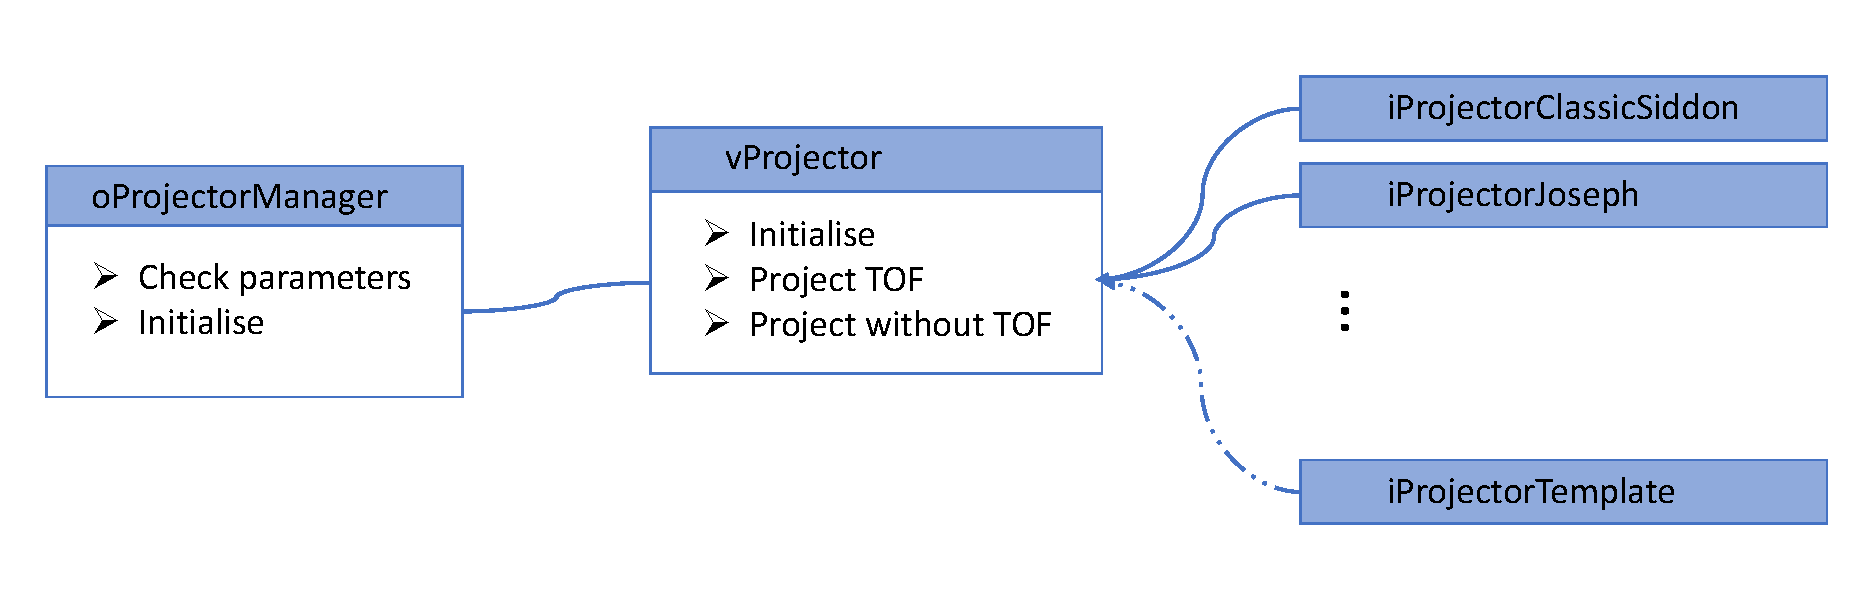
\includegraphics[scale=0.50,angle=0]{2_Theory_Methods/figures/oProjectorManager.pdf}
\caption{Example of \gls{castor} abstraction design for the projection component.} 
\label{fig_2_4:oProjectorManager}
\end{figure}


\section{Datafile}
Data are provided in \gls{castor} in the form of a \gls{castor} datafile, which is based on a generic data description that is identical for both list-mode and histogram data. A "CASToR event" is either a list-mode event or a histogram bin.
The minimum information required for each CASToR event of the datafile are a time-stamp, pair of detector IDs and number of events. Additional information can also be provided per event such as scatter and random corrections, normalisation factors, \gls{tof}, gating information, etc. 

List-mode data maintain the exact timing information of each event. This is advantageous in the reconstruction of dynamic datasets, as the choice of the desired frames for reconstruction is made within \gls{castor}, during reconstruction and using the framing selected by the input of reconstruction parameters. This of course is limited in the case of real data by the corrections used in the reconstruction, which are precomputed using a specific framing definition prior to construction of the CASToR datafile.

Histograms are by definition events that have been histogrammed for a specific time range. All events of a \gls{castor} histogram datafile have the same timestamp which is the timestamp of the first time point of the histogrammed data. Thus dynamic data need to be pre-processed into individual histograms, one histogram per dynamic frame, using a predefined framing definition.
Multiple histograms from a dynamic dataset can be concatenated together into a single file before used in \gls{castor} for dynamic reconstruction. In this case, reconstructions can be performed using the concatenated file and solely with the framing definition used to create the histograms. 
Use of other framing definitions would require re-processing of the data before providing them into \gls{castor} for reconstruction.

In this project, when possible, the use of list-mode datafiles was preferred due to the offered flexibility. 
List-mode datafiles were used for reconstructions of real PET datasets, while histograms were used for reconstructions of simulated datasets (from analytical simulations).

\subsection{Real Data Corrections}
Although in simulations it is relatively easy to get an estimate of corrections, these are harder to obtain for real data. Various estimation methods, as outlined in chapter~\ref{Chap2_1:PET}, are employed by scanner manufacturers to generate corrections that are necessary for quantitatively accurate reconstruction.
CASToR does not provide any functionalities for estimation of corrections. These must be pre-computed and included in the construction process of the castor datafile. 

In this project we made use of real data from GE and Siemens PET systems. Both manufacturers provide offline processing tools (\textit{GE-PET toolbox} for GE systems and \textit{E7 tools} for Siemens systems) for reconstruction, which permit the extraction of corrections.
These tools were used in this project for generation of all the corrections, when using real data in our evaluations.

\section{Geometry}
A generic description of the geometry of an imaging system in \gls{castor} allows for the definition of any \gls{pet} system. Individual detector elements are defined by 3D Cartesian coordinates and an orientation vector. These are pre-computed and input as look-up tables, or are computed by \gls{castor} using a system definition similar to that used for GATE simulations~\cite{Jan2011}.

In this project the geometries of the Signa PET/MR and Siemens mMR PET/MR scanners were used, for which lookup tables are provided with the current version of \gls{castor} (Version 3.1). 

\section{Dynamic aspects}

The use of generic functions and generic datafile definition allows for the reconstruction to be performed by a single implementation of an iterative algorithm. The main steps performed within this iterative algorithm are shown in algorithm~\ref{algo:CASToR_Core}. 

The platform is designed to handle three temporal levels of binning. It makes temporal binning for dynamic frames and binning in two levels of gating (for example cardiac and respiratory motions). %Alternatively, one of the two levels of gating can be used for splitting dynamic data for involuntary motion corrections.

\begin{algorithm} [ht!]
  \For{$i\leftarrow 1$ \KwTo nb of iterations}
  {
   \For{$j\leftarrow 1$ \KwTo nb of subsets}
   {
    \emph{index start}$\leftarrow$ current subset\;
    \emph{index step}$\leftarrow$ number of subsets\;
    Perform Image-based Convolution (forward step)\;
    \tcp{loop over bed positions}
    \For{$s\leftarrow 1$ \KwTo nb of beds}
    {
      \tcp{Parallel loop}\  
      \For{$e\leftarrow$ index start \KwTo nb events \KwStep index step}
      {
        \textbf{Get Event corresponding to }\emph{\textbf{e}}\;
        %Check Image (forward) Deformation for \emph{e}\;
        \If{Deformation required for $e$}{
        Perform Image-Based Deformation(forward step)\;}
        \tcp{apply axial offset for bed}
        \textbf{Apply bed offset}\;
        \tcp{Recover system matrix elements associated with this event}
        \textbf{Compute/load the system matrix elements associated to this Event}\;
        \tcp{Compute the update term associated to the optimization algorithm}
        \textbf{Compute the forward model}\;
        \textbf{Compute the update term(s) to be back-projected}\;
        \textbf{Back-project update term(s)}\;
      }
    }
    %\textbf{Synchronize all data}\;
    Perform Image-based Convolution (backward step)\;
    Perform Image-Based Deformation (backward step)\;
    \textbf{Update image according to the optimization algorithm}\;
    \tcp{Make use of a dynamic model with nested optimisation}
    \If{Nested use of Dynamic model}{
    Estimate/Fit dynamic model \;
    Estimate image from fitted dynamic model \;
    }
   }
  }
\caption{CASToR core iterative loop}
\label{algo:CASToR_Core}
\end{algorithm}

\subsection{Motion correction and image deformation}
Image based deformations can be performed within the iterative loop, over gate bins or sub-frames defined by involuntary motion, that can counteract effects of motion in the data while still using all data (without the need of rejection or individual reconstructions per gate).
Unfortunately, with the current version of \gls{castor} the available implemented deformations are limited to rigid deformation.
Although this deformation can be adequate for brain imaging, it is not suitable for modelling elastic motion that is commonly found in whole body studies. Owing to this limitation at this time, no motion correction was considered in the reconstructions and evaluations performed in this project.

\subsection{Dynamic reconstruction}
Multi-frame reconstruction of individual frames can be performed within \gls{castor} with a single execution. The framing details can be provided in the reconstruction input. For each event, a dynamic switch function is used to identify to which frame the data belongs. Image update is performed accordingly to each respective frame image.

The dynamic series of images is stored in \gls{castor} using a set of temporal basis functions and images of basis coefficients, similar to the description in equation~\ref{eqn:2_3_LinearBasis}. 
In the case of individual frame reconstructions, the set of basis is an identity matrix and the coefficient images are the frame images. 
For dynamic reconstructions using a dynamic model, the model derived basis functions can be used directly in \gls{castor}, in which case the image update terms directly update the parametric images.
But as discussed previously in~\autoref{section:Fully_4D_reconstruction}, dynamic reconstruction can be performed more efficiently when using optimisation transfer principles and nested optimisation for the dynamic model fitting. This functionality was developed in CASToR during this project and details of the implementation are provided in chapter~\ref{Chap3_2:SimStudy}.
%To perform this in \gls{castor} a new component was created (named \textit{oDynamicModelManager}) to handle preparation and fitting of dynamic models. The component and its accompanying abstract and specific classes were developed and tested as part of this project, in collaboration and with guidance by this project participants and Dr Thibaut Merlin.

\section{Multi-bed reconstruction}
\label{chap2_4:MultiBedRecon}
With the generic description of the geometry implemented in CASToR, system matrix elements related to each detection event are computed on-the-fly, by projecting a ray through image space, or they are read from a pre-computed system matrix. 
The on-the-fly computation allows for additional flexibility, which has been used to enable direct multi-bed reconstruction. 
As described in section~\ref{WB_Static_SS}, multi-bed Step and Shoot (SS) acquisitions make use of overlapping beds to increase the sensitivity at the edges of each bed's FOV. The raw PET data for a static WB acquisition comprise of a total number of $n_s$ datasets, one for each bed position $s$. We can represent each bed's raw PET dataset as
%
\begin{equation}
   \bm{y_s} = \Big\{ {y_{si},i=1,...,n_i} \Big\} \\ . \\
\end{equation}
%
%
By incorporating the offset of each bed position in the projection operation, equation~\ref{eqn:MLEM} can be re-written for direct reconstruction of the whole acquisition effective \gls{fov}, using all acquired raw data, as
\begin{equation}
\lambda_j^{(k+1)} = \frac{\lambda_j^{(k)}}{\sum_{s=1}^{n_s} \sum_{i=1}^{n_i} P_{sij}} 
\sum_{s=1}^{n_s} \sum_{i=1}^{n_i} P_{sij} 
\frac{y_{si}}{\sum_{d=1}^{n_j} P_{sid}\lambda_d^{(k)} + C_{si} } \\ , \\
\label{eqn2_4:MLEM_multibed}
\end{equation} 

where now the image $\bm{\lambda}$ has the dimensions of the whole effective \gls{fov}, and the additive correction terms $C_{si}$ is provided for each respective bed position $s$. 

Direct reconstruction of multi-bed data, which combines data from overlapping acquisitions within the iterative reconstruction loop, improves the statistics of the overlapping region that are available for each iteration. It has been shown that this technique can result in improved contrast to noise ratios at the overlapping regions, for specific levels of acquisition statistics~\cite{Ross2004}. 

This method has been implemented in CASToR by making use of an additional loop over bed positions and an "Apply bed offset" function, as seen in the CASToR iterative algorithm~\ref{algo:CASToR_Core}, which applies the bed offset to the projector for the events of each bed~\cite{Stute2014}.


\iffalse
\begin{figure}[htp]
    \centering
    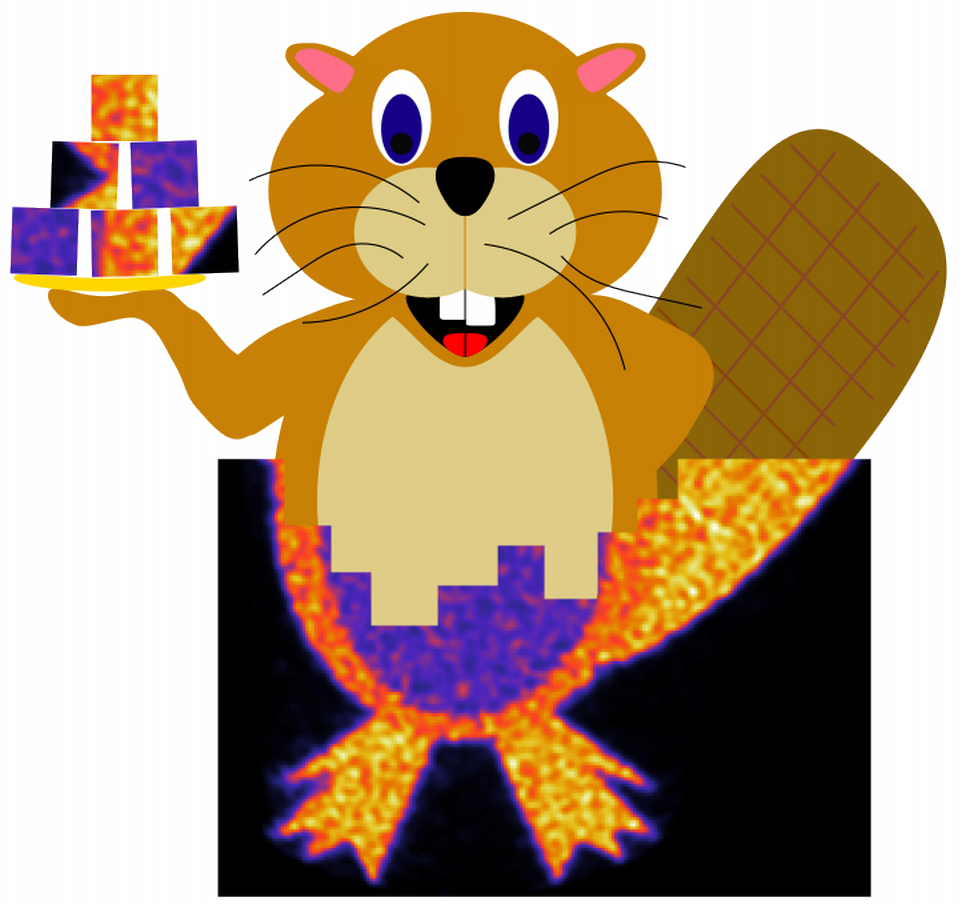
\includegraphics[width=5cm]{2_Theory_Methods/figures/CASToR_logo_transparent_cut.png}
    \caption{Customizable and Advanced Software for Tomographic Reconstruction}
    \label{fig:galaxy}
\end{figure}
\fi
    
    \part{Contributions}
    %\chapter{Results}


\chapter{Multi-bed Dynamic Whole Body PET: Acquisition optimization}
\section{Introduction}
In PET imaging one of the needs in many clinical and research applications is the acquisition of information over the whole body. Moreover, dynamic information over the whole body can allow for research applications of PET, such as in pharmacokinetics, to expand to the whole body and enable potential future clinical applications. 
But an important limitation of DWB protocols in scanners with limited A-FOV is the result of temporal gaps in the acquired data of any given bed position.
In practice for scanners that have no in-build DWB protocols, such as the Signa PET/MR, a large fraction of the temporal gaps in DWB protocols can be attributed to a greater extend to system processes that are launched automatically between WB sweeps rather than to time taken to move the bed between bed positions. These processes include the transfer of raw data files and reconstructions performed during scanning. %More acquisition time could be gained if those could be avoided and temporal gaps were decreased. 
Reducing these system delays is therefore of prime importance for reducing temporal gaps in the data.

In this chapter, we review results of acquisition performance for a DWB protocol implemented on the Signa PET/MR scanner as part of the IsotoPK pharmacokinetic study~\cite{Marie2019}. A short introduction on the design of the protocol using current scanner features is provided, with additional details on the protocol and data processing of this protocol's data provided in Appendix~\ref{chap:AppendixA}.
We then describe the implementation of an experimental fully-automated protocol for DWB acquisitions on the Signa PET/MR, that was designed with the aim of reducing acquisition delays and allowing for greater flexibility in the selection of bed positions. The development of this protocol was conducted in collaboration with GE Healthcare, as part of this PhD project (which was also a milestone within \gls{hybrid}). 
Finally, we present results from the use of the experimental acquisition protocol on a \glsfirst{nhp} study and compare against the standard DWB protocol used in the IsotoPK study using data from fourteen volunteer scans.

\section{Methods \& Results}
\subsection{Design of IsotoPK DWB protocol on the Signa PET/MR}
Prior to commencing this PhD project and in perpetration for the IsotoPK study, a DWB protocol was designed on the GE Signa PET/MR scanner. The desired axial coverage was achieved using 5 bed positions and a reduced overlap, as shown in diagram (C) of figure~\ref{fig3_1:BodyCoverage}. The relatively small overlap (half compared to routine clinical protocols) was selected to reduce the number of beds and subsequently the acquisition temporal gaps.
The study design was limited to a total duration of 1 hour from injection and includes an initial dynamic single bed (DSB) phase centred over the liver, where the highest expression of the transporters under study was expected. 
The DSB position was imaged for 3 minutes from injection, prior to the start of DWB acquisition.
Because the system has no in-build protocols for DWB imaging, a custom protocol had to be made using a sequence of static WB acquisitions. Each WB pass had to be individually pre-planned, which resulted in hard-coded bed positions (identical positions for all subjects, relevant to a reference mark). Each volunteer positioning was made using a chest-landmark, with no further adjustments of the protocol being possible for the optimum arrangement of the bed positions, relative to each patient's size.

For the design of the framing used in the IsotoPK DWB protocol, the following empirical metric has been taken under consideration. We define the Delays to Acquisition ratio (DAR) as the ratio of total delays to acquisition time for every WB sweep, using the relationship
\begin{equation} \label{eqn:acq_to_dead_time}
 \mathrm{DAR}(n_s) = \frac{dl_{bed}\cdot (n_s-1) + dl_{Sweep}^{(n_s)}}{t_{duration}\cdot n_s }  \\ , \\ 
\end{equation}
where $n_s$ is the number of beds in the acquisition, $t_{duration}$ is the frame duration for a single bed of the WB sweep, $dl_{bed}$ the delays between adjacent beds and $dl_{Sweep}^{(n_s)}$ the delay between WB sweeps (for a DWB protocol of $n_s$ bed positions). This relationship is based on the assumption that all beds in a WB sweep have the same frame duration.
First estimations of the delay times for the Signa PET/MR had shown a delay of approximately 6 seconds between adjacent bed positions and 20 seconds between WB sweeps. Using this information, the framing sequence shown in table~\ref{tab:IsotoPK_Framing} was chosen with the shortest frame duration set to 20 seconds in order to maintain a DAR below 50\% at the early phases of the DWB study. 

\begin{table}[ht!]
\centering
\caption{Framing of IsotoPK DWB protocol.}
\label{tab:IsotoPK_Framing}
\begin{tabular}{|l|l|l|l|l|}
\toprule
\textbf{Phase ID} & \textbf{Description}              & \textbf{Frame Duration (s)} & \textbf{Number of frames} & \textbf{DAR} \\
\textbf{} & \textbf{} & \textbf{} & \textbf{per bed position} & \textbf{} \\
\midrule
1        & DSB & 10                 & 18        & N/A                 \\
2        & DWB                      & 20                 & 9         & 44\%                \\
3        & DWB                      & 30                 & 8         & 29\%                \\
4        & DWB                      & 40                 & 2         & 22\%                \\
\bottomrule
\end{tabular}
\end{table}

The MR sequences required for attenuation correction (MRACs) were performed prior to injection and during the DWB protocol acquisition. The first MRAC sequence at each bed location lasted approximately 35 seconds (conducted prior to injection), with subsequent scans over the same locations lasting approximately 21 seconds per bed. This difference in time requirements between initial and subsequent MRAC sequences is caused by the MR shimming sequences that are performed before MR imaging. At first, shimming is conducted in full to optimise MR homogeneity, while only a faster shimming update is conducted on subsequent scans of the same bed positions.
MRAC acquisitions were not repeated for all WB sweeps of the DWB protocol, to allow for staff entry in the room for blood sampling which is required for the derivation of the input function and metabolite analysis. 

The acquired DWB data were initially reconstructed at the system console.
Then, as part of this PhD project, the raw data were retrospectively exported for offline processing and reconstruction with \gls{castor}, using an automated pipeline which is described in Appendix~\ref{chap:AppendixA}.

\subsection{Results from IsotoPK study}

The result beds positions of the DWB protocol can be seen in figures~\ref{fig3_1:ctrl_mips} and ~\ref{fig3_1:rif_mips} for the included fourteen studies from the IsotoPK protocol.
Using the timing information of the extracted raw PET data, the average delay times per imaged subject were estimated, shown in the form of box-plots for $dl_{bed}$ in figure~\ref{fig3_1:BoxPlots_beds} and for $dl_{Sweep}^{(5)}$ in figure~\ref{fig3_1:BoxPlots_sweeps}.

It is noteworthy that with the accumulation of experience in using the PET/MR system for performing the DWB protocol, the delays between sweeps were reduced considerably, which can be seen by comparing the most recent examinations against the first. This can be attributed in part to improved preparation of the PET/MR system before performing the protocol (ex. reboot of the system prior to study, etc.). Before this practice was established, as the system software has not been designed for acquiring multiple whole-body passes many system crashes had been experienced using this custom protocol. These have caused losses of acquisition time (which has not been included in this evaluation) and also resulted in differences in the number of WB passes per subject. Secondly, in part, the reduction in delays can be attributed to improved staff training on the use of the protocol and awareness of common problems.
%
%
\begin{figure} [ht!]
\centering
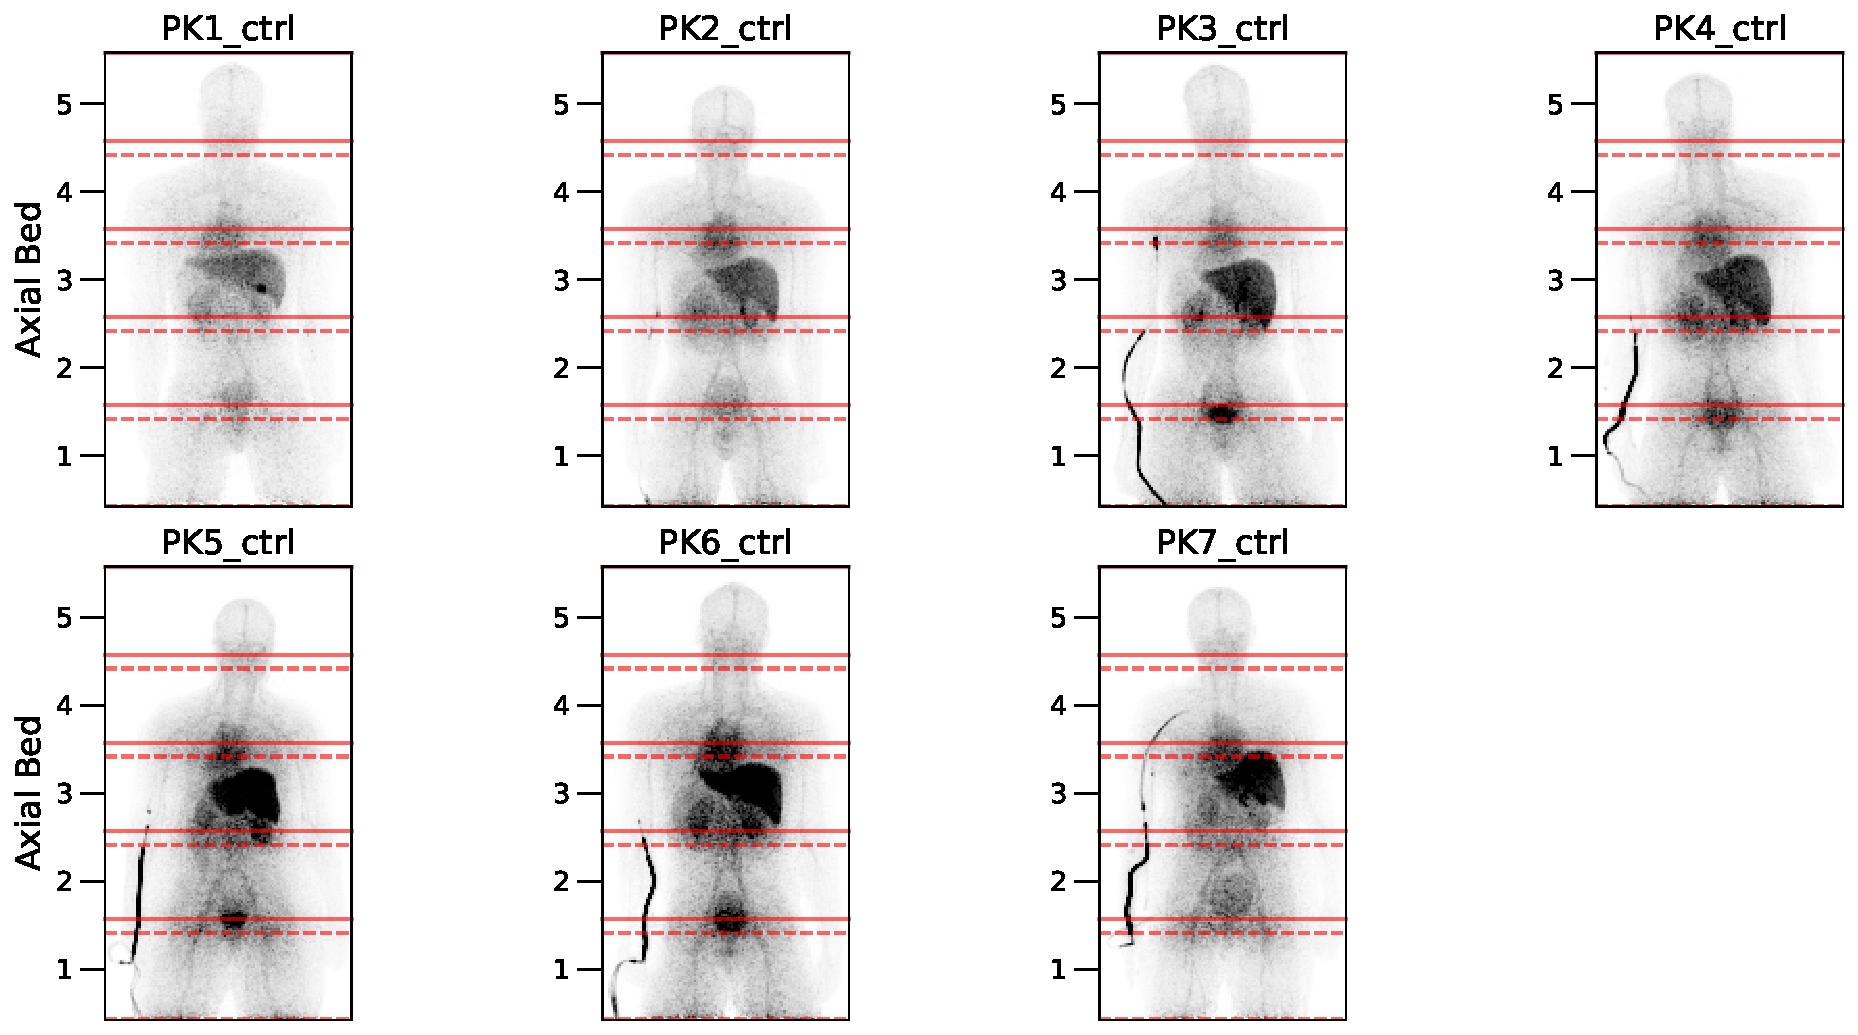
\includegraphics[scale=0.5,angle=0]{3_Results/3_1_DWB_Optimization/figures/3_1_MIPS_ctrl.pdf}
\caption{Coronal MIP projections of 7 volunteer control DWB scans with overlay of axial bed start (\protect\tikz[baseline]{\protect\draw[line width=0.5mm] (0,.8ex)--++(1,0) ;}) and end (\protect\tikz[baseline]{\protect\draw[line width=0.5mm,densely dashed] (0,.8ex)--++(1,0) ;}) location.} 
%TODO: Add over-scan in the CBM D-WB protocols. 
\label{fig3_1:ctrl_mips}
\end{figure}
%
\begin{figure} [ht!]
\centering
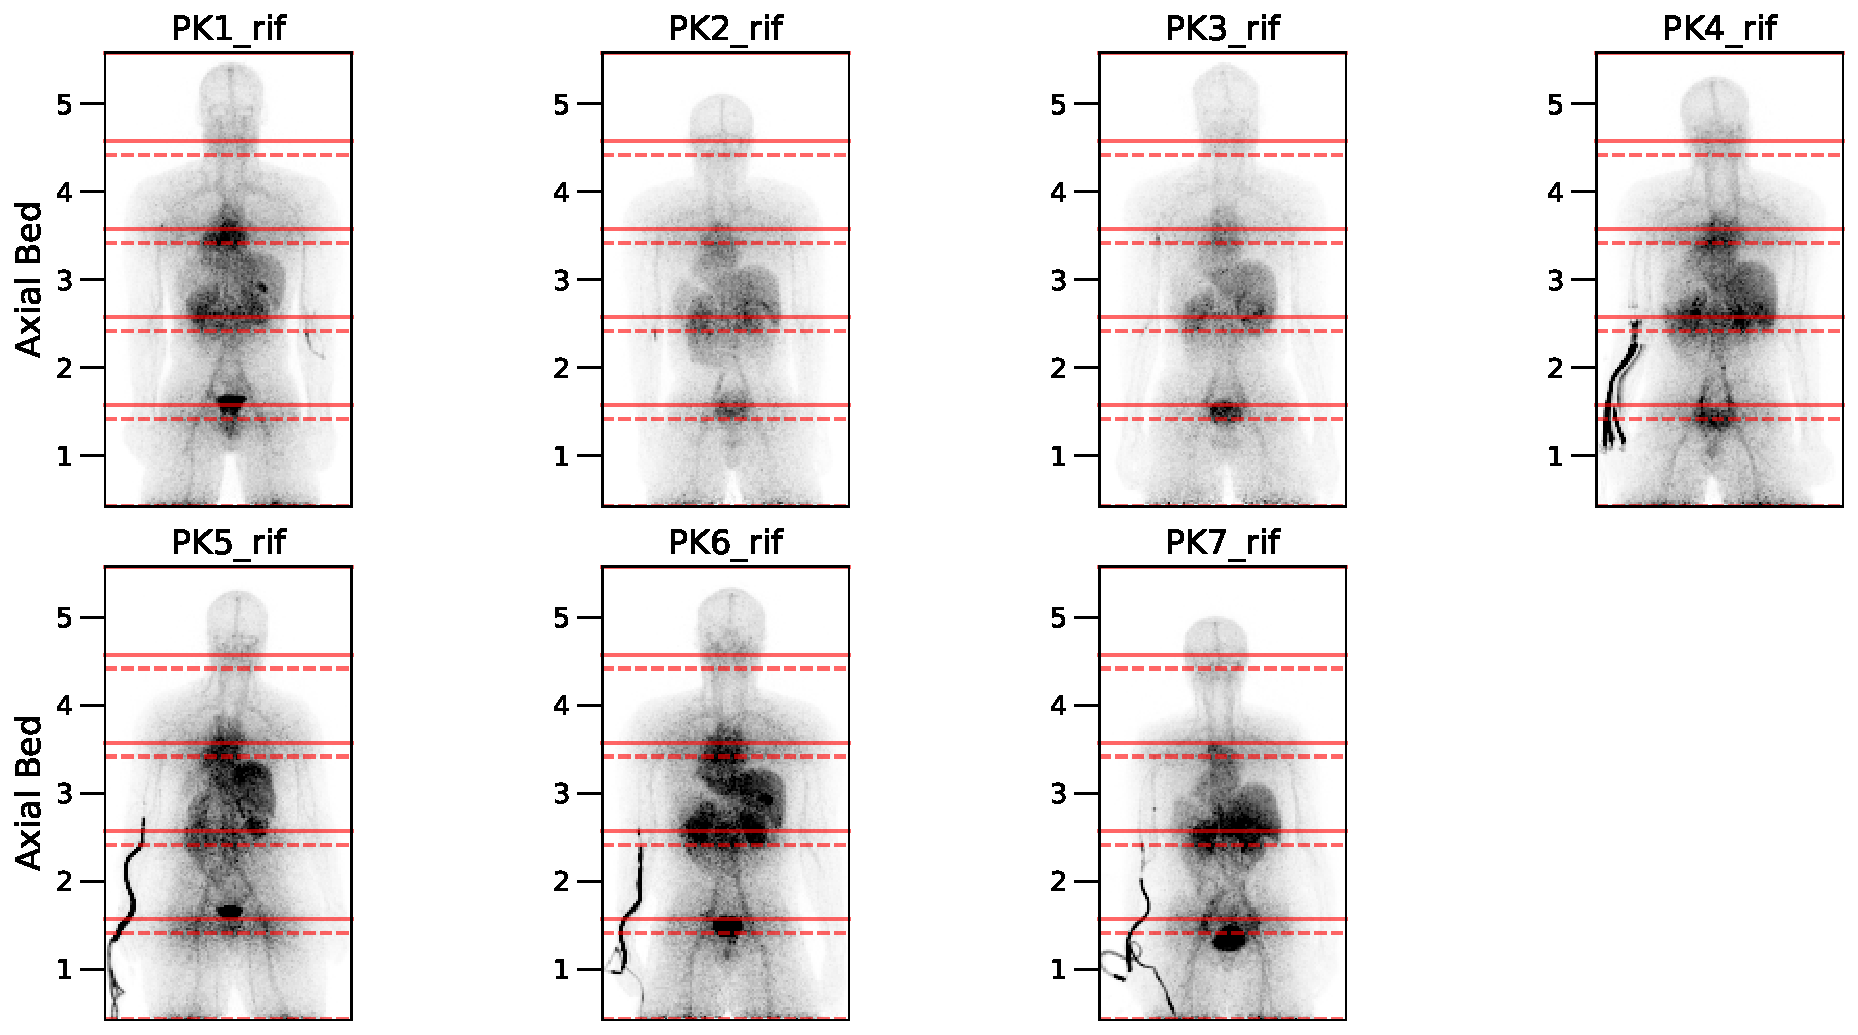
\includegraphics[scale=0.5,angle=0]{3_Results/3_1_DWB_Optimization/figures/3_1_MIPS_rif.pdf}
\caption{Coronal MIP projections of 7 volunteer rif DWB scans with overlay of axial bed start (\protect\tikz[baseline]{\protect\draw[line width=0.5mm] (0,.8ex)--++(1,0) ;}) and end (\protect\tikz[baseline]{\protect\draw[line width=0.5mm,densely dashed] (0,.8ex)--++(1,0) ;}) location.} 
%TODO: Add over-scan in the CBM DWB protocols. 
\label{fig3_1:rif_mips}
\end{figure}
%
For the 3 more recent subject examinations the average intra-bed delay time ${dl_{bed}}$ was 5.69 s (95\%CI: 5.63, 5.75) and the average delay time between sweeps $dl_{Sweep}^{(5)}$ was 26.17 s (95\%CI: 26.13, 26.22).
This measured average $dl_{Sweep}^{(5)}$ value is slightly higher than the value considered in the design of the protocol. With these average measurements, the DAR for the WB sweeps of beds with 20 s frame duration becomes approximately 49\%. \\
%
\begin{figure} [ht!]
\centering
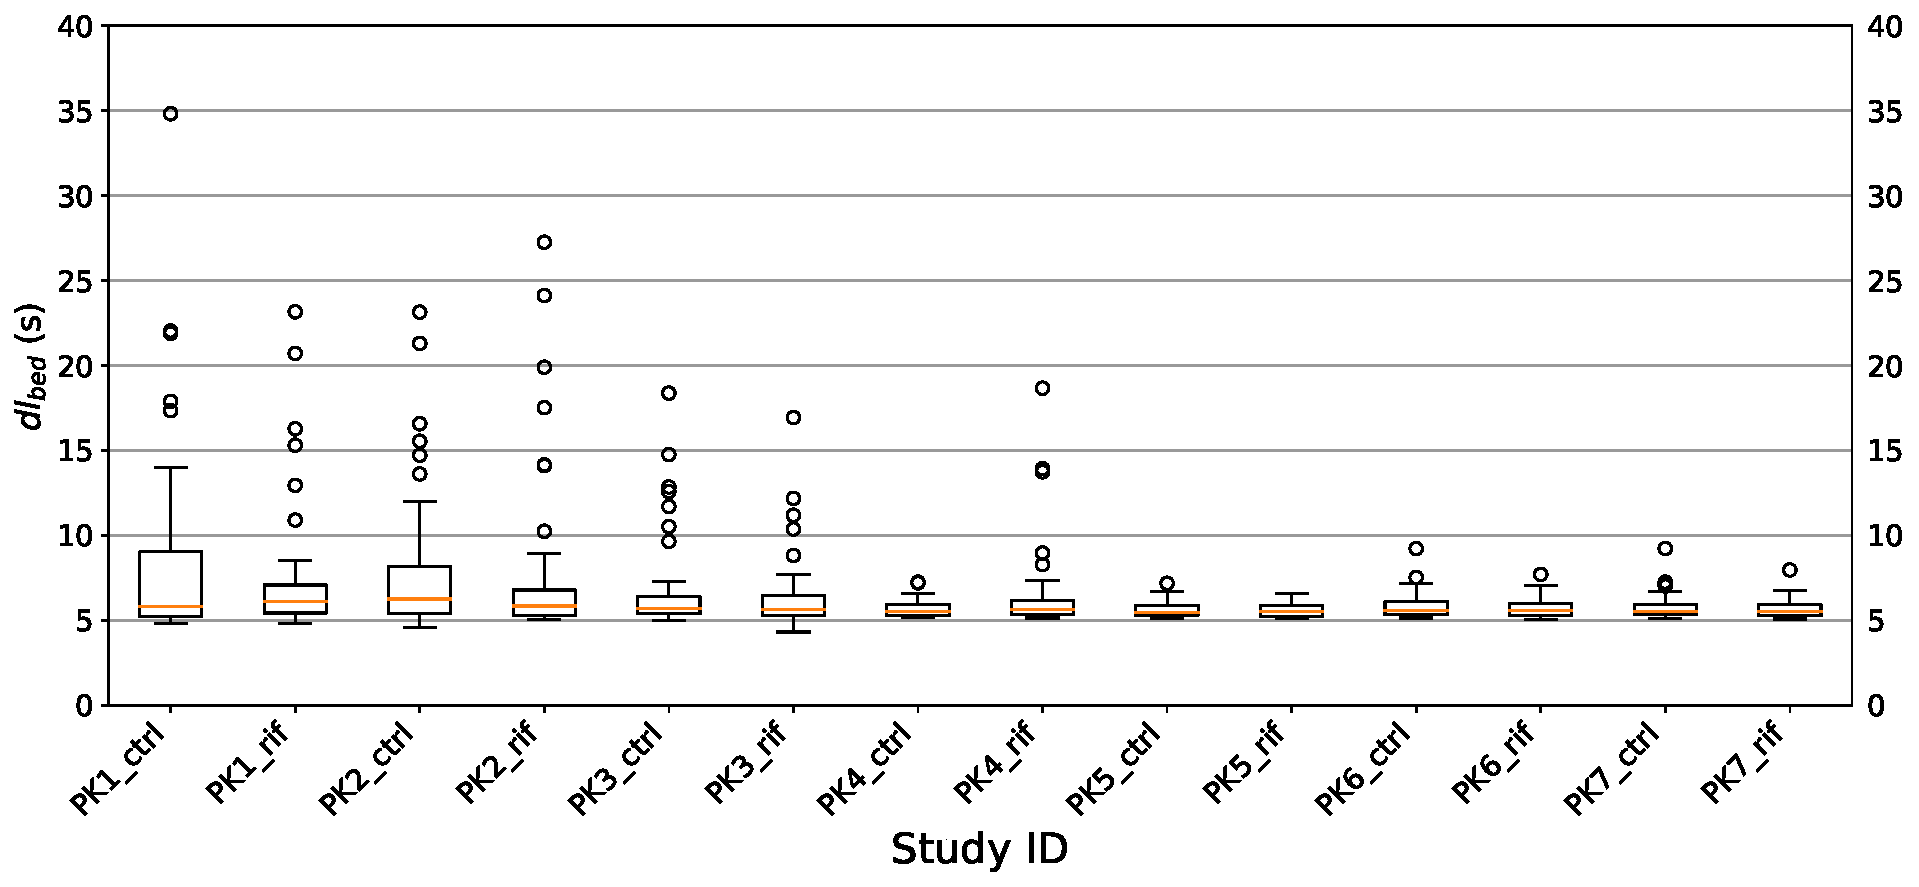
\includegraphics[scale=0.5,angle=0]{3_Results/3_1_DWB_Optimization/figures/3_1_BoxPlots_DTBeds.pdf}
\caption{Box plots of intra-bed delays $dl_{bed}$ of the IsotoPK DWB protocol used in practice.} 
%TODO: Add over-scan in the CBM D-WB protocols. 
\label{fig3_1:BoxPlots_beds}
\end{figure}
%
\begin{figure} [ht!]
\centering
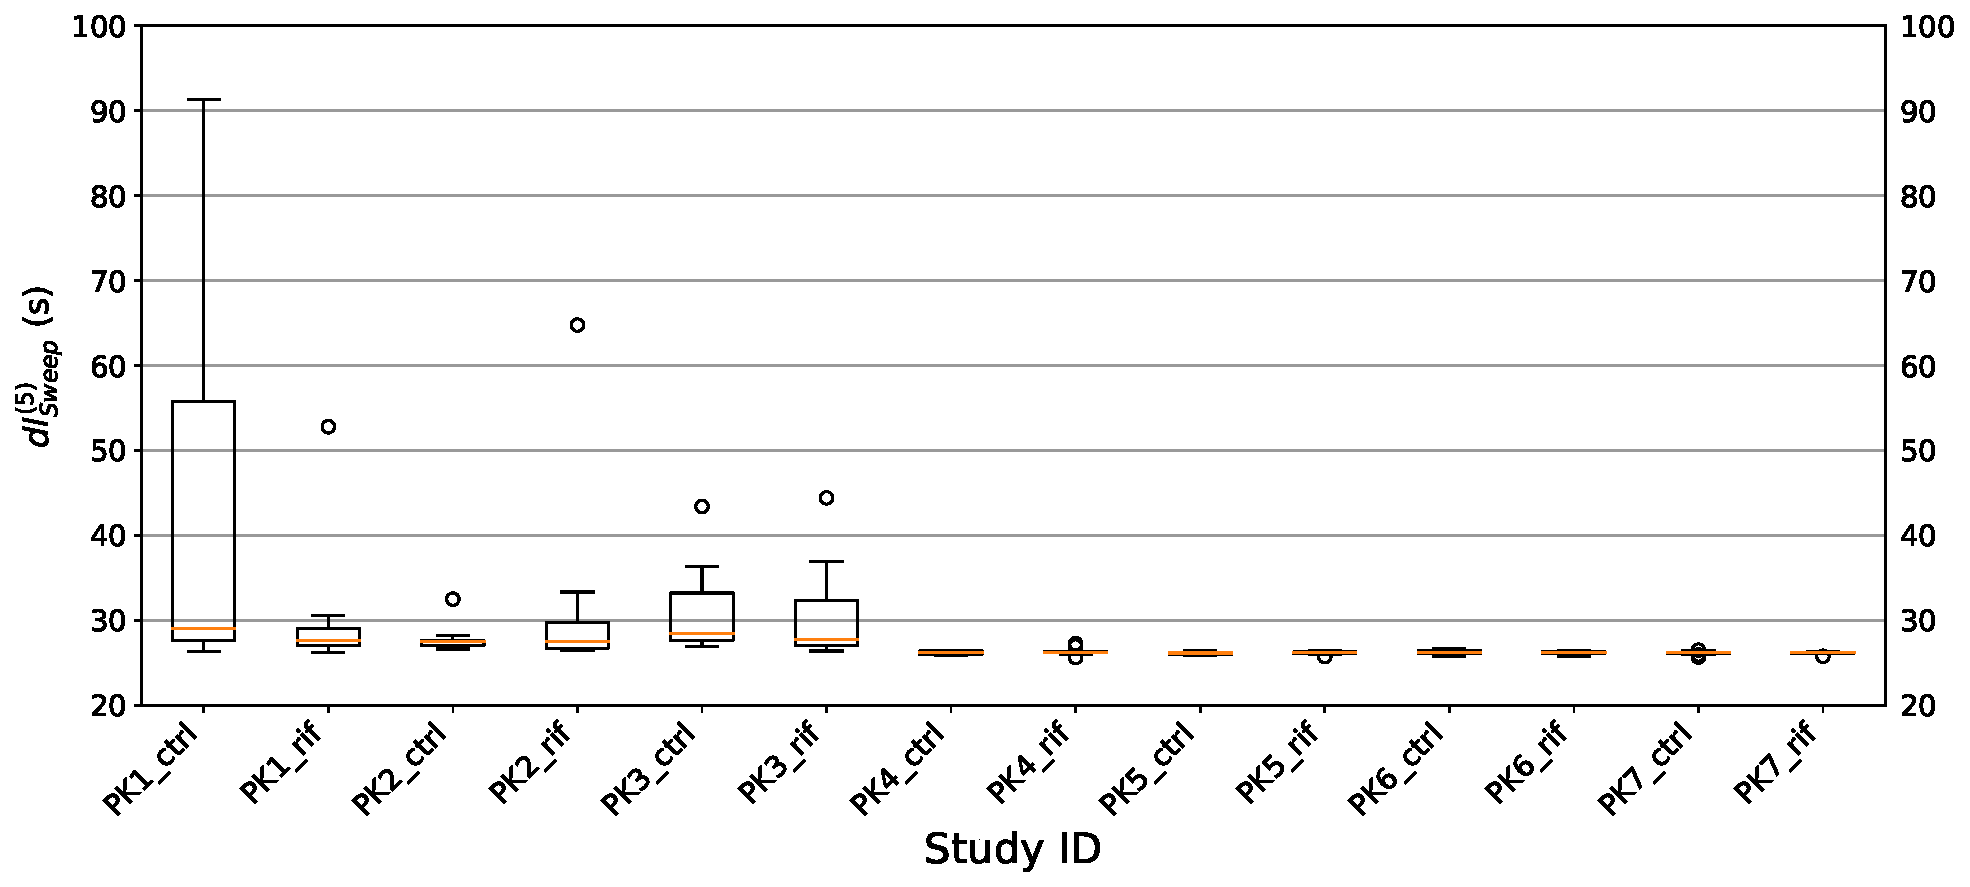
\includegraphics[scale=0.5,angle=0]{3_Results/3_1_DWB_Optimization/figures/3_1_BoxPlots_DTSweeps.pdf}
\caption{Box plots of delay between WB Sweeps $dl_{Sweep}$ of the IsotoPK DWB protocol used in practice.}
%TODO: Add over-scan in the CBM D-WB protocols. 
\label{fig3_1:BoxPlots_sweeps}
\end{figure}
%
%
%
\subsection{Design of a fully-automated DWB protocol on the Signa PET/MR}
Part of this PhD project was allocated for the development of a fully automated DWB protocol on the Signa PET/MR. 
The main requirement for the envisioned protocol was to allow for continuous capture of PET data during DWB acquisition, into a single list-mode file for all bed positions and WB sweeps. Then the data would be processed after the acquisition, split into individual data for each bed position and reconstructed with the correct bed positional information. Using such an acquisition strategy, the delays between bed positions and WB sweeps could be brought down to the time taken by the physical motion of the scanner table alone. 

Towards this goal a three week secondment was planned at factory facilities of GE healthcare (Waukesha, Wisconsin, USA). %with the opportunity the gain insights on the operations of the Signa PET-MR scanner. 
There with help of the PET/MR team it was made possible to exploit in-build factory tools of the Signa PET/MR for the purposes of DWB automation. The two key tools necessary were: 
\begin{itemize}
    \item\textbf{Table Emulation} \\
    This tool allows for disassociation of the table position between the MR and PET systems. It is the key tool that allows for the PET system to acquire continuously, while the MR system governs table motion. A disadvantage of this functionality is that once table emulation is enabled MR acquisitions cannot be performed.% while acquiring PET data.
    \item\textbf{Table Motion} \\
    This tool commands the MR system to execute movements of the scanner bed. It can be used to drive the bed to a target location at a desired speed. 
\end{itemize}

The automated DWB protocol was implemented as a Python class because the Python programming language is available on the PET/MR system's console and allowed for easy integration of the system tools with our custom made routines, all under a common system clock for accurate timing of bed movements and registration of events.
The protocol was named "Auto-IsotoPK", but despite its name is a generic DWB protocol that is not limited to the IsotoPK pharmacokinetic study. It allows for an optional DSB scan to be acquired before starting the DWB acquisition. The protocol also allows for any number of beds to be used for DWB acquisition, with custom positioning of the beds for each examination using an initial MR scout image. 
Because MR acquisitions cannot be performed after \textit{Table Emulation} is enabled, all bed position MRACs must be acquired before the PET examination and used for all WB sweeps of the study.
A short \gls{sop} on the operation of the protocol is given in Appendix~\ref{chap:AppendixA}.

After the procedure is completed, the whole PET study is stored as a single list-mode file, but without bed positional information. The precise timing information of the acquired bed positions is saved in a separate log file, which is used for post-processing the data and separation of the bed positions before reconstruction.  

\subsection{Results from NHP study}
After initial tests using phantoms, the automated DWB protocol was tested on an actual pre-clinical DWB study. A macaque was scanned under full sedation with a novel [$^{18}$F]Crizotinib tracer. Crizotinib is an anti-cancer drug used in the therapy of \gls{nsclc}.
The DWB study was conducted to examine the tracer uptake in the brain as well as uptake and excretion from other organs. The macaque was injected with 185 \si{\mega \becquerel} of the novel tracer. Directly after injection an initial DSB scan was conducted, centred over the brain for a duration of 90 s, followed by DWB acquisition of three bed positions. The study was planned for an approximate total duration of one hour. A total of 28 WB sweeps were fitted in the study, with the framing of 3$\times$10~{s}, 5$\times$20~{s}, 5$\times$30~{s}, 5$\times$45~{s}, 10$\times$60~{s} for each of the three bed positions.

Acquisition of the required MRACs was performed prior to injection, at the planned bed positions shown in figure~\ref{fig3_1:Macaque_MRI}. In this acquisition, only the body coil of the PET-MR system was used, which is optimised for use with the human body size. Their use resulted in sub-optimal quality of MR images and generated attenuation maps. The attenuation maps were edited manually before being used for PET data reconstruction.

\begin{figure} [ht!]
\centering
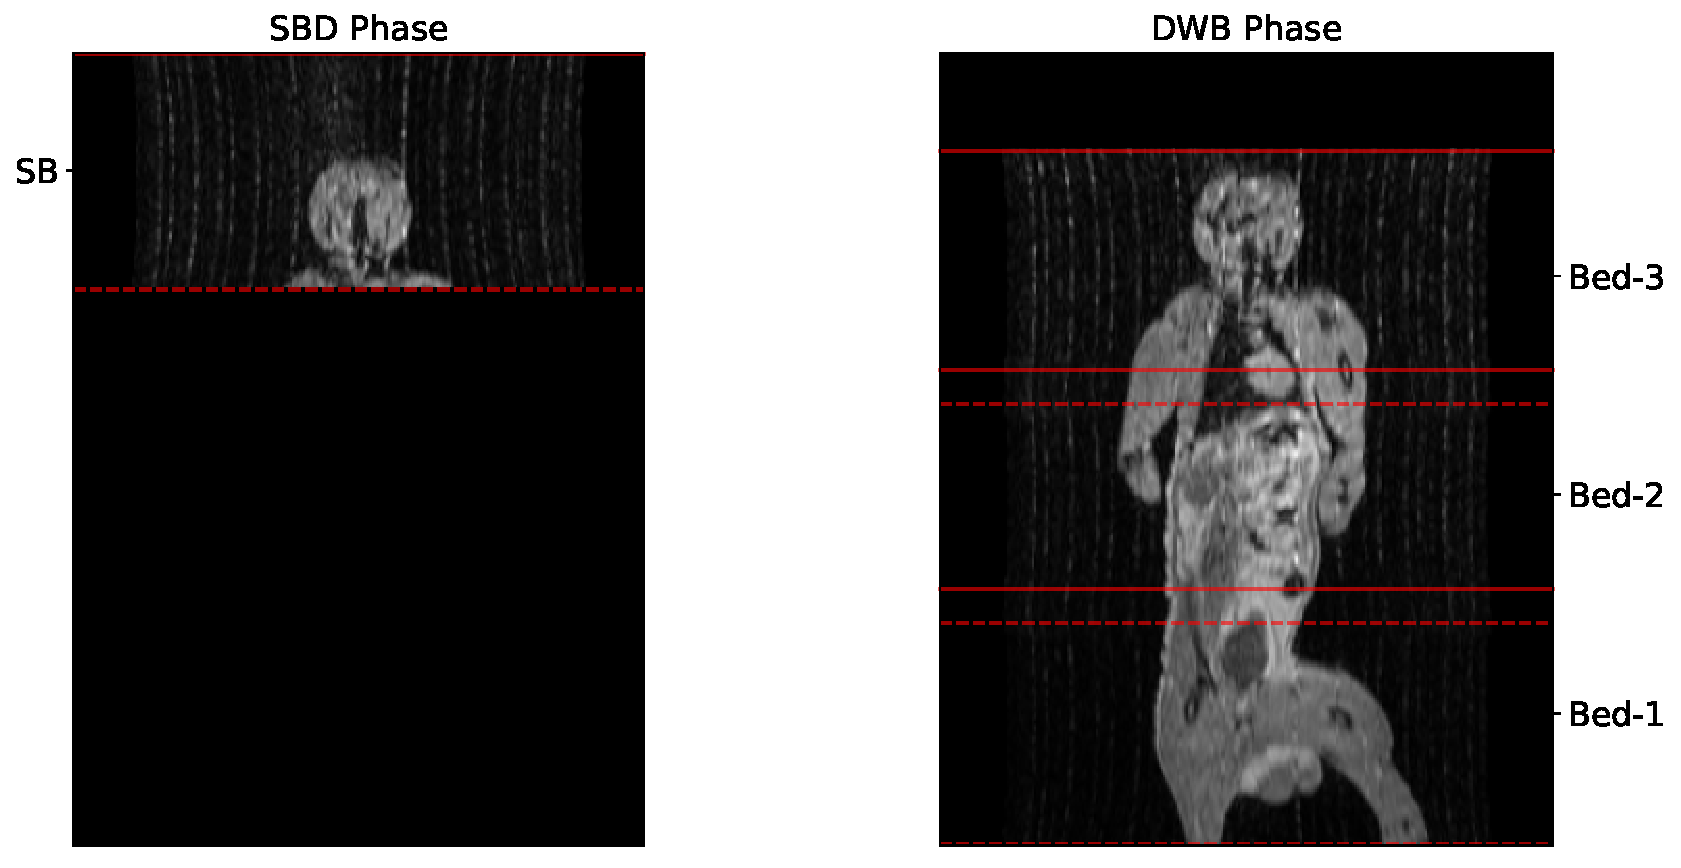
\includegraphics[scale=0.5,angle=0]{3_Results/3_1_DWB_Optimization/figures/3_1_Macaque_MRI.pdf}
\caption{MRAC acquisitions of NHP study showing the planned bed positions of the two acquisition phases, with overlay of axial bed start (\protect\tikz[baseline]{\protect\draw[line width=0.5mm] (0,.8ex)--++(1,0) ;}) and end (\protect\tikz[baseline]{\protect\draw[line width=0.5mm,densely dashed] (0,.8ex)--++(1,0) ;}) location.}
\label{fig3_1:Macaque_MRI}
\end{figure}

The complete study dataset was recorded in a single list-mode file, of which the head curve (curve of prompts rate with time) can be seen in figure~\ref{fig3_1:Macaque_Head_Curve}. By overlaying the recorded timing information over this curve, the two phases of the acquisition (DSB and DWB), as well as the three bed position of the DWB acquisition, can be distinguished. The initial 260 seconds of the recorded list-data's head curve with the overlaid phases and bed positions are shown in figure~\ref{fig3_1:Macaque_Head_Curve_Phases}. 

\begin{figure} [ht!]
\centering
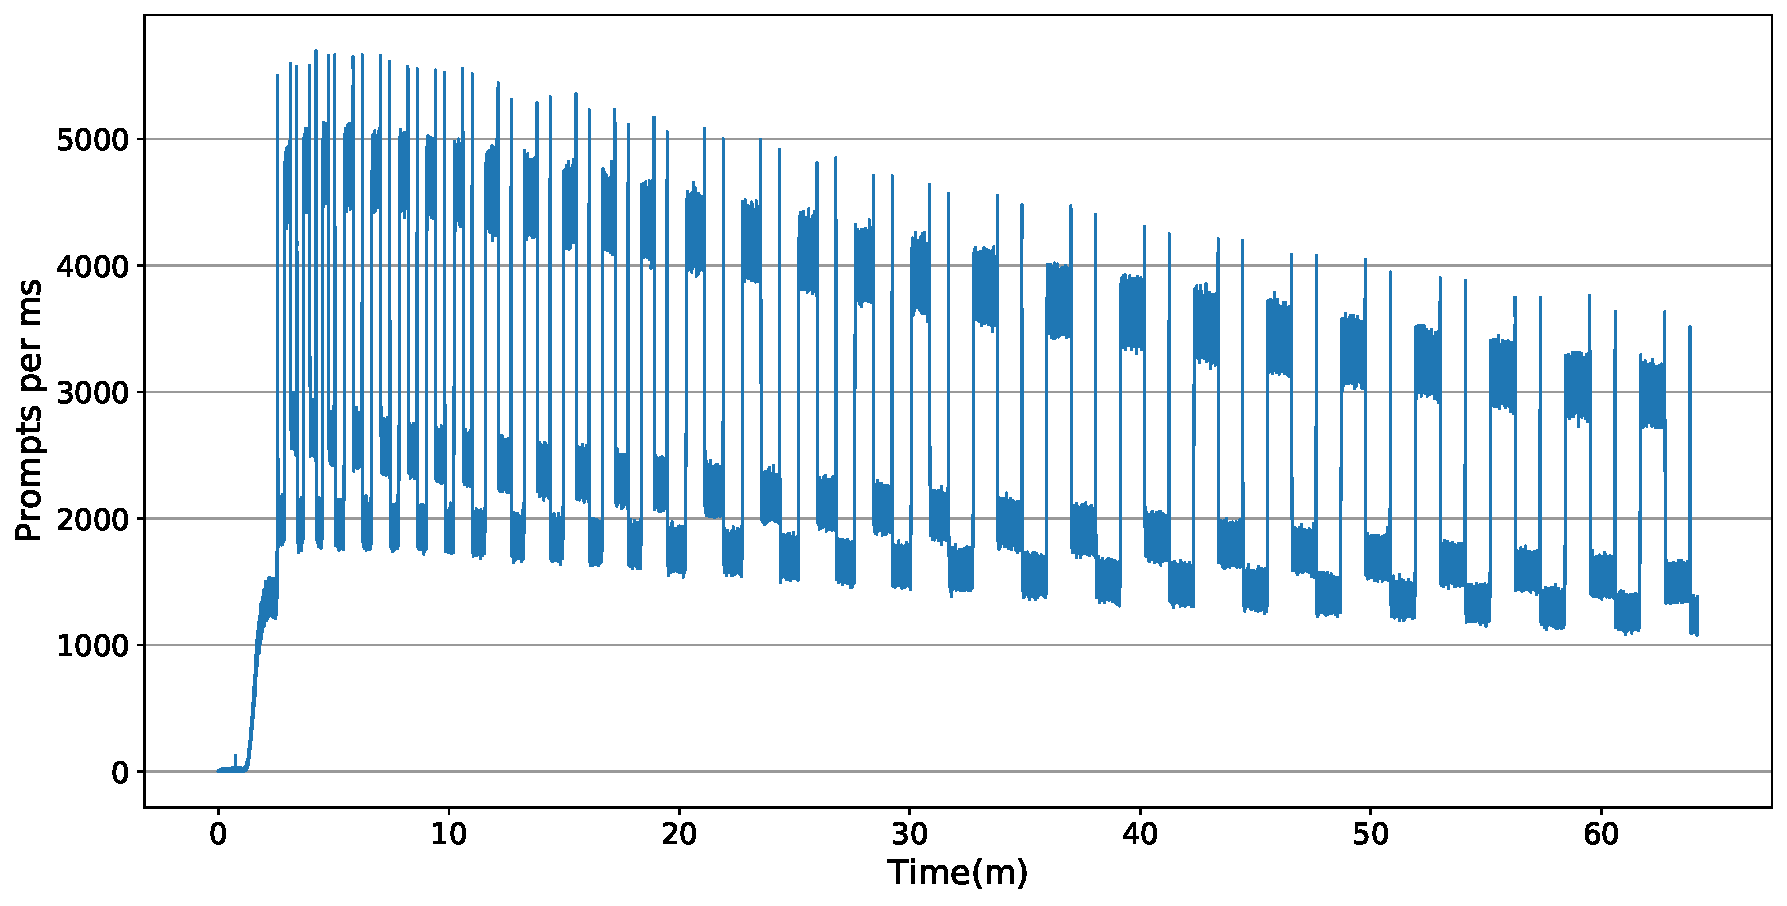
\includegraphics[scale=0.45,angle=0]{3_Results/3_1_DWB_Optimization/figures/3_1_Macaque_Head_Curve.pdf}
\caption{Head curve (prompts rate against time) of the acquired NHP study data in a single list-mode file using the fully-automated protocol.}
\label{fig3_1:Macaque_Head_Curve}
\end{figure}

\begin{figure} [ht!]
\centering
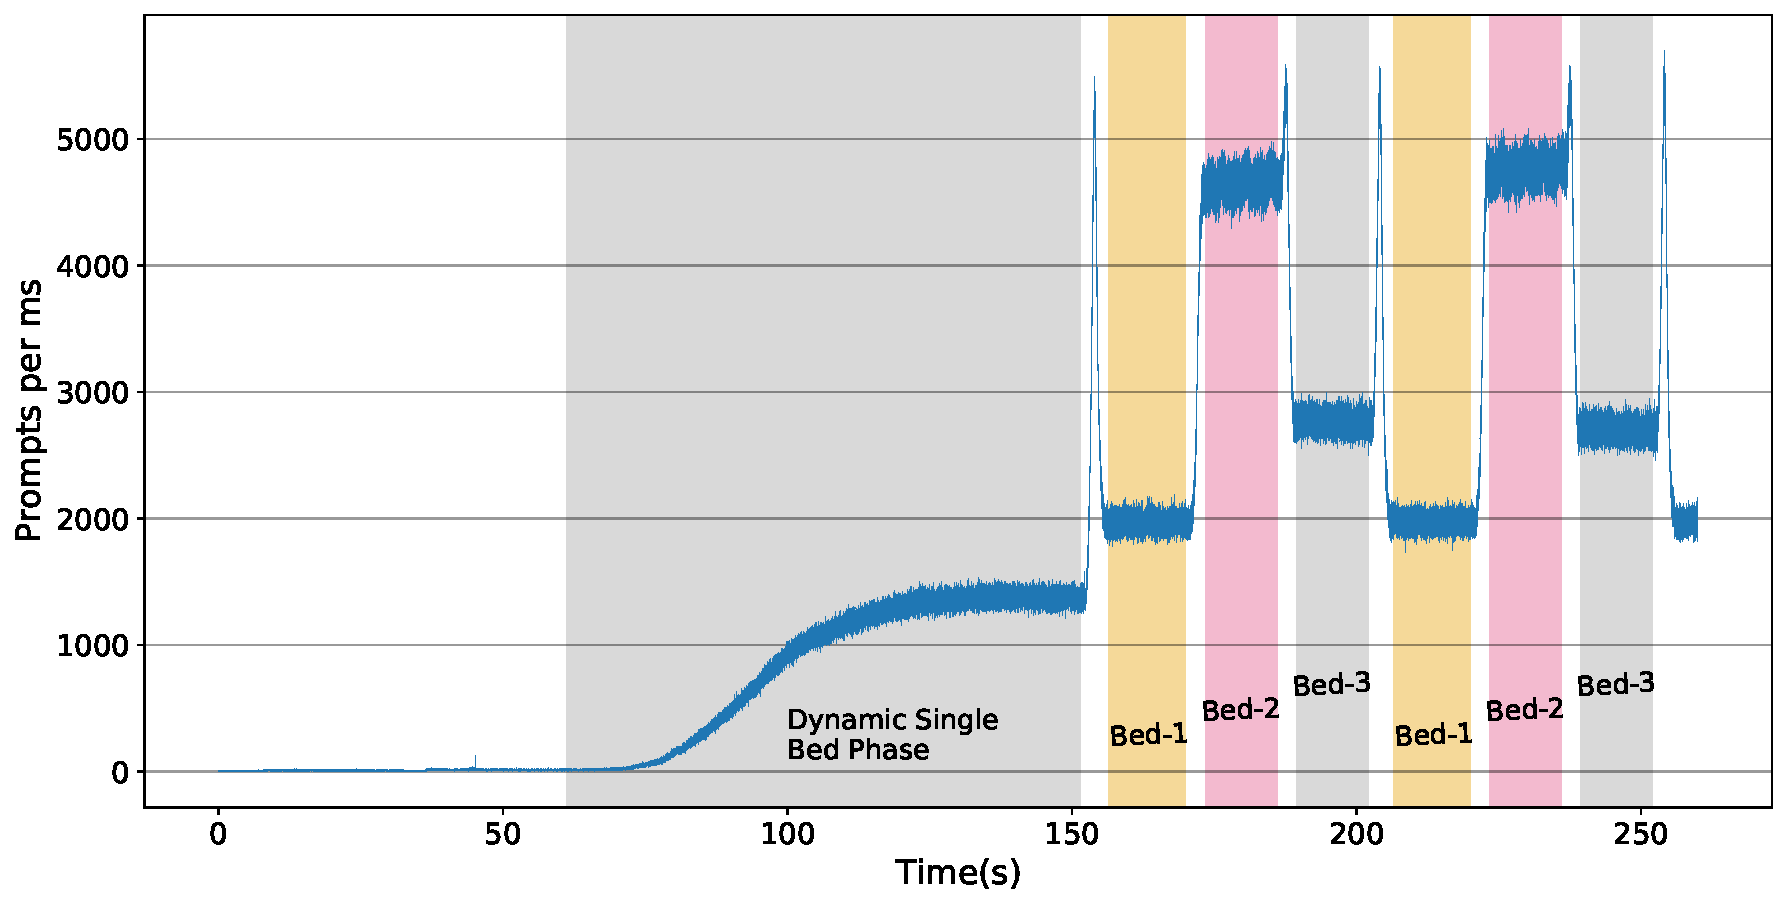
\includegraphics[scale=0.45,angle=0]{3_Results/3_1_DWB_Optimization/figures/3_1_Macaque_Head_curve_Phases.pdf}
\caption{Head curve (prompts rate against time) of the acquired NHP study showing the DSB and DWB phases of the acquisition and the three DWB bed positions.}
\label{fig3_1:Macaque_Head_Curve_Phases}
\end{figure}
%
Using the timing information recorded in the acquisition log file, the data were split into four individual bed position datasets (one from DSB and three from DWB) and were processed with the GE-PET toolbox as individual single bed dynamic studies, to generate corrections necessary for reconstructions using \gls{castor}. The list-mode data along with the generated corrections were then converted into the CASToR data-file format for subsequent reconstruction tests. A coronal \gls{mip} view of 3D reconstructions (averaged across all dynamic frames) is shown in figure~\ref{fig3_1:Macaque_PET}. \\
An \gls{idif} was estimated from the reconstructed PET data. A right carotid \gls{voi}, that was visible on both phases of the acquisition, and a left ventricle \gls{voi} on the Bed-3 position were used for the estimation. Both VOIs provided similar blood activity values for the DWB phase and were averaged to produce the final \gls{idif}, shown in figure~\ref{fig3_1:Macaque_PET_input_function}. This test showed that extraction of an \gls{idif}, using multiple VOIs on both phases of the acquisition was possible and in good agreement between the used VOIs.
%
\begin{figure} [ht!]
\centering
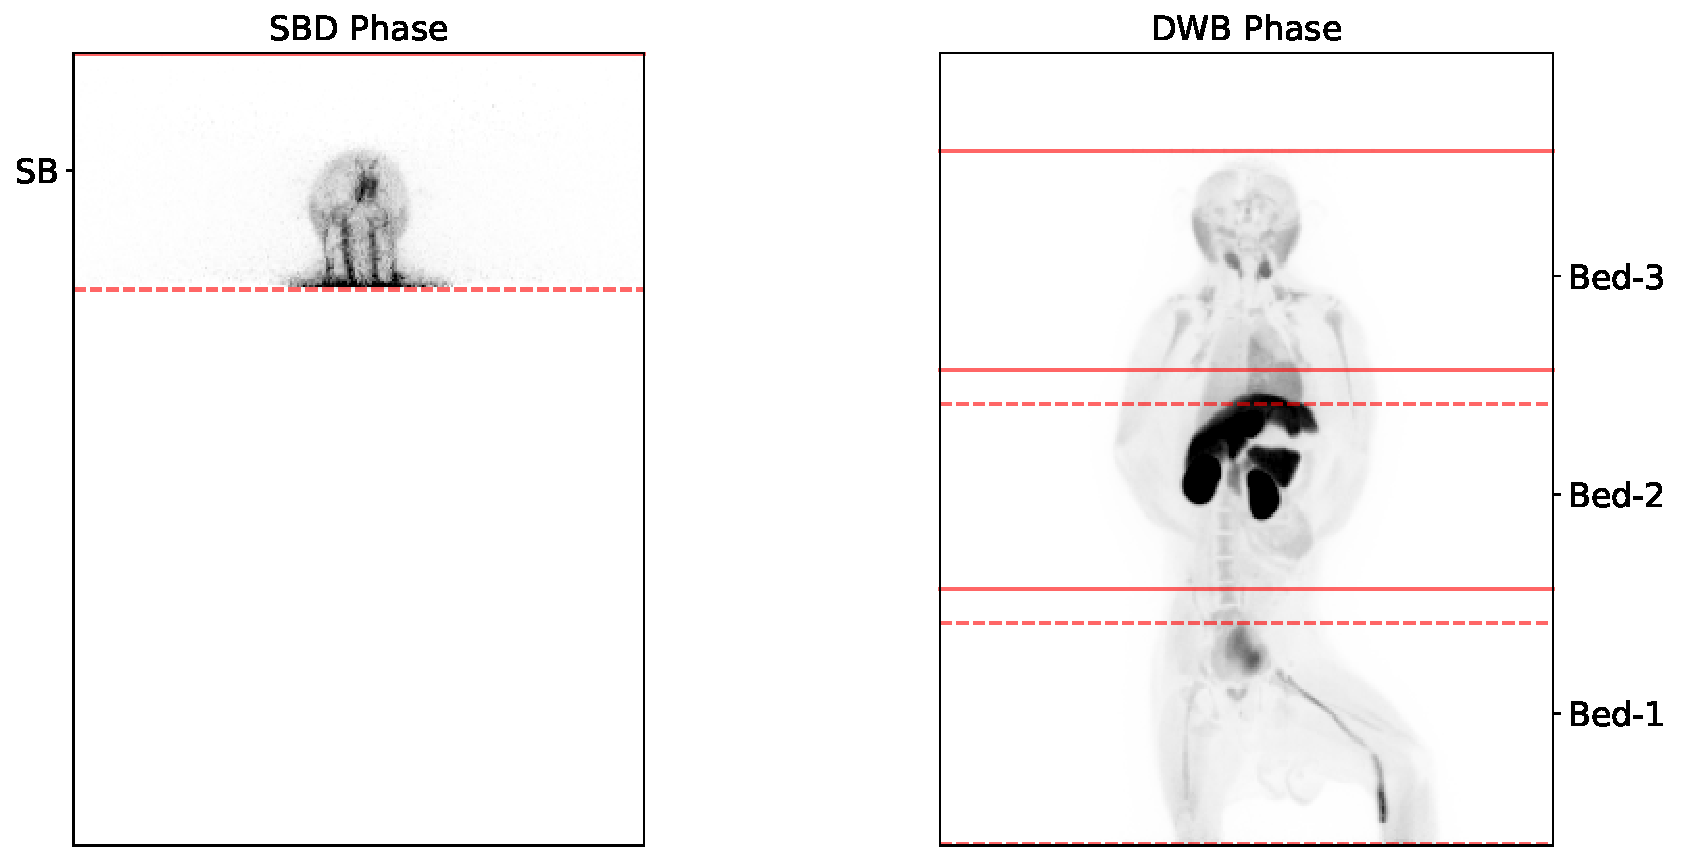
\includegraphics[scale=0.45,angle=0]{3_Results/3_1_DWB_Optimization/figures/3_1_Macaque_PET.pdf}
\caption{Coronal MIP views of the NHP study's reconstructed PET images, for the two phases of the acquisition, with overlay of axial bed start (\protect\tikz[baseline]{\protect\draw[line width=0.5mm] (0,.8ex)--++(1,0) ;}) and end (\protect\tikz[baseline]{\protect\draw[line width=0.5mm,densely dashed] (0,.8ex)--++(1,0) ;}) location.}
\label{fig3_1:Macaque_PET}
\end{figure}
%
%
\begin{figure} [ht!]
\centering
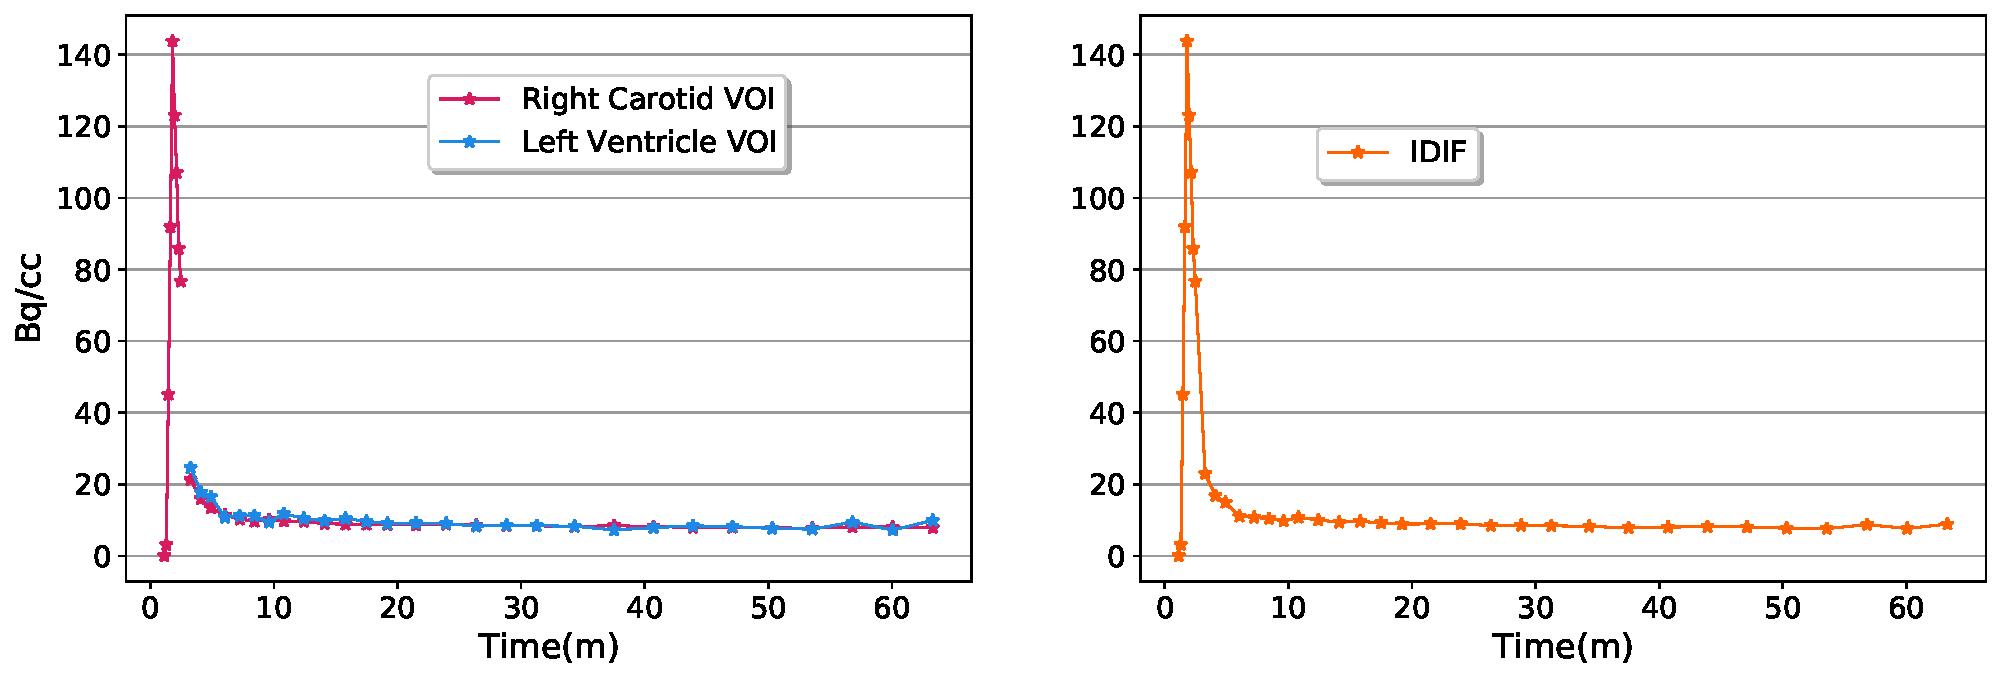
\includegraphics[scale=0.45,angle=0]{3_Results/3_1_DWB_Optimization/figures/3_1_NHP_InputFunction.pdf}
\caption{NHP study's image derived input function using information from multiple bed positions.}
\label{fig3_1:Macaque_PET_input_function}
\end{figure}
%
Finally, an estimation of the delays (time gaps) for this single NHP study using the automated acquisition protocol was made using log timing information. The results showed an average intra-bed delay time $dl_{bed}$ of 3.77 s (95\%CI: 3.62, 3.91) and an average delay time between sweeps $dl_{Sweep}^{(3)}$ of \mbox{4.6 s (95\%CI: 4.53, 4.67).} 

\section{Comparison of protocols}
The design and implementation of the fully-automated DWB protocol was made with the intentions of reducing delay times, compared to the custom implementation of a DWB protocol for the IsotoPK study. 
Before direct comparison of the protocols, the measured delay times between WB sweeps need to be adjusted to account for the difference in the number of bed positions between the two assessed protocols. 
Assuming a linear relationship between delays due to bed motion and the number of beds, the following relationship can be expressed
%
\begin{equation} \label{eqn:acq_to_dead_time_ratio}
dl_{{Sweep}}^{(5)} =\ \frac{5}{3} dl_{{Sweep}}^{(3)}  \\ , \\ 
\end{equation}
%
where now $dl_{Sweep}^{(5)}$ is the assumed delay between sweeps that would be achieved by the fully automated protocol for DWB imaging of 5 bed positions.
It is expected that this value is an overestimation of the delays that would be achieved by the fully-automated protocol as the delays due to bed motion include an acceleration and deceleration phase that impacts shorter bed movements greater than longer movements.
Using the measurements from the NHP study, the estimated $dl_{Sweep}^{(5)}$ that could be achieved is 7.66 s. 
Using this value we can estimate that the DAR for 20 s frames can be reduced from 49\% to approximately 22.7\%, by use of the fully automated protocol instead of the current IsotoPK DWB protocol. Furthermore, using the reduced $dl_{Sweep}^{(5)}$ delays a DAR of approximately 45.5\% can be achieved for 10 s frames, allowing for more frequent sampling in the early phases of DWB acquisition without significantly compromising the quantity of acquired statistics.

Additionally, besides the reduced acquisition gaps, the fully automated protocol allows for more flexibility in the arrangement of bed positions for DWB imaging. By contrast, the hard-set bed positions of the IsotoPK DWB protocol do not always allow for optimum use of the effective A-FOV in each examination, as seen for example in examination PK2 in figures~\ref{fig3_1:ctrl_mips}~and~\ref{fig3_1:rif_mips}. In some cases, a lesser number of bed positions might be adequate and preferable as it would lead to a substantial increase of sampling frequency per bed.

\section{Discussion}

As seen by the reduction of acquisition delay times and reduction of DAR for short frame duration, the implementation of the fully-automated DWB protocol allows for improved DWB imaging with reduced acquisition temporal gaps.
%
This gain can be used towards improving acquisition statistics by reducing the DAR ratio and towards a higher sampling frequency of early frames. 
A limitation in this assessment is that the comparisons were based on the empirical metric of DAR, without relating directly to the final kinetic analysis performed on the data and produced parametric images. In practice, faster sampling could also be achieved with larger acquisition gaps at the cost of reduced acquisition statistics and vice versa with higher statistics achieved at the cost of reduced sampling frequency. 
These trade-offs are expected to affect mostly kinetic estimations that are sensitive to fast dynamic information shortly after injection. 
Ideally, the DWB acquisition protocol should be optimised for the expected kinetics under study and the parameters of interest. Nevertheless, towards this optimisation, the developed fully-automated protocol can allow for greater variability in the available trade-off options of acquisition statistics vs. sampling frequency of early frames. 
Another aspect where fast sampling can be beneficial is for the derivation of the \gls{idif} from DWB data. Given the fast initial sampling that can be achieved using a fully-automated protocol, it is possible to reduce the initial DSB acquisition duration or potentially remove it completely while still sampling frequently enough for an estimation of the \gls{idif}.
In the \gls{nhp} application presented in this chapter we showed that it is possible to combine \glspl{idif} from multiple VOIs and from both DSB and DWB phases, without need for an identical bed position between the two acquisition phases. This flexibility can also allow flexibility in the DSB position placement over the WB scan, without compromising the derivation of the \gls{idif}. 

Additionally, another consideration that needs to be accounted for concerning fast sampling of early frames is the acquisition of MRAC sequences. For the Signa PET/MR the fastest MRAC sequence is performed in approximately 21 seconds (including preparation sequences) and as such shorter PET frames would have to be conducted without MRACs. In the IsotoPK DWB protocol, multiple MRACs are acquired in order to best account for any potential subject motion in the attenuation correction used for each WB pass. Their use can also be potentially expanded to the investigation of motion correction techniques. But if motion can be assumed to be small and negligible, then multiple MRACs would not be required and shorter PET frames can be acquired using MRACs acquired prior to injection. 

In this evaluation, a practical limitation that has not been considered is safety limits on table movement that are needed to avoid undesirable effects from electromagnetic induction on patients/volunteers, which are caused by the fast movement of the bed within the MR field. For the tests conducted on the NHP, these limits have not been considered. These limits are expected to reduce the speed that would be permissive for human subjects, in compliance also with patient comfort requirements, and thus reduce to some degree the potential gains from the use of the fully automated DWB protocol. 

In our tests we have considered only the use of S\&S acquisition in the implementation and optimisation of DWB protocols. 
In a previous study on DWB protocols utilising CBM acquisition, advantages favouring the use CBM acquisition for DWB protocols were seen~\cite{Karakatsanis2016a}. Beyond the aspects of reduced acquisition delays, CBM offers other benefits such as uniform axial sensitivity of acquisition, flexibility in sampling frequency by adjustments in table speed within each WB sweep, improved patient comfort, etc. 
Overall, use of CBM naturally overcomes many of the limitations posed by the use of multi-bed DWB protocols and S\&S acquisition. 
Additionally, CBM protocols can also allow for bi-directional motion that eliminates delays between WB sweeps. 
These acquisition modes, their effects on acquisition gaps and result parametric image quality were considered further in the simulation study presented in chapter~\ref{Chap3_2:SimStudy}.
Using the fully automated protocol and the developed tools we were able to emulate a CBM acquisition for the \gls{nhp} study, by selecting a relatively slow table speeds and recording PET data continuously. But normalization and quantitative reconstruction of the acquired CBM datasets is a demanding, task as previously described~\cite{Panin2014}, and thus quantitative reconstruction of these data was not considered further in this PhD project.

Overall the implementation of this fully automated protocol serves as proof of concept for flexible bed position placement and selection of frames duration, being limited only by the bed speed of the GE Signa PET/MR and not by software or other system components. This protocol is a significant improvement from the currently used DWB protocol of the IsotoPK study. As the system has not been designed with DWB capabilities, the current DWB protocol involves manual planning of each WB sweep, multiple delays in data transfers and individual WB sweep reconstructions, etc. 

However, the automated method does not allow for bed positional information to be recorded in the raw data and necessitate ad-hoc techniques to record bed positions and bed movements in separate files. These limitations necessitate custom processing steps to be performed after acquisition and prior to reconstruction, to allow for accurate and quantitative reconstruction of the acquired data. 
Furthermore, the current implementation of the automated protocol does not allow for MRI to be acquired during PET acquisition. Although a mixed acquisition using the automated protocol and the current implemented DWB protocol could allow for MR in the acquisition, it would further increase complexity and risk of system failures.

Due to the discussed limitations of the automated protocol and the considerations for safety, it was not used for subsequent DWB acquisitions within the IsotoPK study and was not considered further in the context of this thesis. It served only as a proof of concept for future developments.

\section{Conclusion}
A fully automated DWB protocol was developed on the GE Signa PET/MR as a proof of concept for fully automated and flexible acquisition of DWB imaging, recorded on a single list-mode file for the whole study. 
Data using this protocol were successfully acquired, processed and reconstructed in a test NHP study.
Use of the protocol allowed for considerable reduction of delay times, enabling faster sampling without loss of PET data statistics.
Thanks to the automated protocol, the minimum bed frame duration can be reduced from 20 to 10 s while maintaining the same DAR , compared to the DWB protocol currently in use.
A considerable limitation of the implementation of this protocol is the unavailability of the MR system for MRI acquisitions during the DWB acquisition, which is caused by the bespoke utilities on which our experimental protocol was based upon.
Finally, further considerations of permissible table speeds for patient safety and comfort need to be applied before using this protocol on human subjects.

%At this moment CBM protocols are not available on the PET/MR scanner, but DWB protocols based on CBM acquisition can overcome many of the limitations and enable even more flexibility in acquisition frequency, with the additional benefits of uniform axial sampling. 

%\subsection{Auto-IsotoPK: Continuous Bed Motion on the Signa PET-MR}
%The flexibility offered by the use of the automated protocol and the dedicated \"Table Motion\" tool allowed for testing the proof of concept of CBM on the Signa PET-MR scanner. Although this acquisition mode is not supported by the system, we emulated the acquisition of a single whole-body sweep by commanding a table movement at a speed of \SI{5}{\milli\metre\per\second}. The duration of the total sweep, that covered the three bed positions that were acquired in the previous DWB study and included an 50\% overscan, was ...

%\iffalse
\chapter{Implementation of dynamic functions in CASToR and dynamic simulator}

\begin{itemize}
    \item  How dynamic reconstruction was implemented in CASToR (in relation to the methods explained in the theory section). \\
    \item  How dynamic models were implemented in simulation. Short demonstration of simulation and reconstruction using a custom phantom from real mMR data.  \\
\end{itemize}

\chapter{Simulation Study}
The gap paper and expand if time permits. Describe more on spectral model and $K1$ and micro-parameters comparison also. \\

\chapter{Advancements in WB and WB-Dynamic reconstruction}
\label{chap:Results_CASToR}
\begin{itemize}
\item  All the déjà unique implementations in CASTOR. \\
\item  Theory and practice for Dynamic Whole Body reconstruction (direct and nested), with toy simulation example and macaque data. \\
    \item All the works with real data , single and multi bed.  \\ 
    \item The use of the Spectral model and offered advantages in pharmacokinetic studies. \\
\end{itemize}

\chapter{Other projects: HYBRID, CASToR etc.}
All the other projects within Hybrid ! \\
\begin{itemize}
    \item Laura's Simulation \& CNN \\
    \item Lalith's MoCo mMR Brain GAN. \\
\end{itemize}

%\fi
    
    \chapter*{Conclusions and prospects}
The objective of this thesis was to explore and assess methods for improving whole-body parametric imaging, for clinical and pharmacokinetic applications, using multi-bed dynamic whole body PET/MRI data.
As hybrid PET/MR scanners and the majority of other PET systems provide only a limited axial field-of-view (FOV), dynamic whole-body (DWB) protocols are used to extend the effective FOV over the required axial length. But these acquisitions come at the cost of limitations in acquisition counts and sampling frequency that degrade parametric image quality and accuracy.
Several aspects were investigated, throughout the process of DWB data acquisition to data processing and reconstruction. We largely focused on the use of dynamic reconstruction algorithms for improving the use of the PET acquired data in the estimation of activity and parametric images.

Specifically, in this project we have
\begin{enumerate}
\item Developed an optimised protocol for S\&S mutli-bed DWB acquisitions on the Signa PET/MR.
\item Evaluated and compared novel dynamic reconstruction algorithms for whole-body parametric imaging, with focus in oncological imaging.
\item Explored the use of a direct multi-bed dynamic reconstruction framework on a real WB pharmacokinetic study.
\item Evaluated the use of adaptive residual modeling applied in DWB data and a generic dynamic reconstruction algorithm.
\end{enumerate}

Firstly, we have worked closely with the manufacturer of the GE Signa PET/MR in methods for reducing the loss of counts and sampling frequency in DWB imaging by means of reducing delays in the acquisition process. This resulted in a custom fully-automated protocol that has shown to considerably reduce delays when applied on a real DWB study on a \gls{nhp} subject. However, approval for use of this protocol with human studies requires a more thorough review of safety measures and closer collaboration with the manufacturer. Ideally, CBM acquisition techniques should also be considered for implementation as they can contribute further towards improvements and flexibility in acquisition. 

Secondly, we made use of dynamic reconstruction for DWB parametric imaging, with focus on oncology applications of dynamic FDG PET and Patlak parametric imaging, using simulated and real data.
We proposed the use of an indirect method for DWB parametric imaging based on the spectral analysis model and dynamic reconstruction which allows for generic compartmental modelling to be used during reconstruction for temporal regularisation. While the Patlak model is limited to data after steady state conditions have been reached, this novel spectral reconstruction approach enables the use of all dynamic data in the reconstruction and offers greater modelling flexibility. Post-reconstruction Patlak parametric imaging using the regularised data of the spectral reconstruction outperformed direct Patlak dynamic reconstruction. But even this method did result in high parametric image noise when reconstruction was iterated sufficiently to ensure accurate quantification. Potentials for improvement should be examined further using additional regularisation methods to deliver acceptable parametric image noise for clinical applications and ensure accurate quantification.
%All the reconstruction methods used in this work were implemented in the open source and fully quantitative reconstruction platform CASToR and are available in the current public release of CASToR. 
Finally, we have expanded our application of dynamic reconstruction to real data from an exploratory, first in man, WB pharmacokinetic study. We extended the use of the dynamic reconstruction to direct multi-bed reconstruction, which enabled the use of the complete DWB dataset within a single iterative loop for dynamic reconstruction. This approach inherently handles the individual bed position data's sensitivity and timing information, notably for the bed overlapping positions where previously suggested practices made use of compromising solutions. In this type of applications, the use of spectral reconstruction is favoured as it does not impose strong assumptions on the unknown underlying kinetics. Preliminary results using VOI based analysis showed good agreement with results from 3D regular reconstruction. These applications also enabled the generation of surrogate parametric K1 maps, for relative comparison between scans.
Further comparisons with post-reconstruction parametric imaging need to be conducted to explore the reliability and additional benefits of this reconstruction approach towards accurate parametric imaging, but these were not conducted at this preliminary stage of the study.
In this application, we identified a limitation in the modelling process over the bladder, that had the potential to be the source of spatially propagating errors within the dynamic reconstruction process. 
To minimise this risk we have included an adaptive residual modelling approach within the reconstruction. This method identified and selectively corrected the model activity estimates over the poorly modelled bladder region, which provided a significant reduction of model fit errors at the cost of added noise over the entire FOV. Some optimisation advancements were made using pre-treatment of residual data, but further developments are needed for reducing the induction of noise by this approach. 

A major limitation in the application of dynamic reconstruction on WB data is motion and motion induced artefacts that affect image quality and quantification. 
In the setting of DWB imaging, complex motion exists in the PET data that ideally needs to be accounted for and corrected for within the reconstruction process. 
Many approaches for including motion correction in the reconstruction have been proposed and successfully used. But estimation of the underlying elastic motion vectors over time and over the WB is a challenging task. Moreover, the limited sampling of MR and PET in DWB acquisitions reduces the sensitivity of many data-driven approaches for motion estimation. In our evaluations, using PET raw data and MR data from attenuation correction sequences, we were unable to use common motion estimation tools for the successful estimation of elastic motion vectors.
Recently there has been a plethora of applications of Machine Learning (ML) in medical imaging, including motion estimation and motion correction.
The increasing use of ML approaches for motion estimation could lead to further developments that could be useful in the DWB motion estimation problem.

During the course of this project, the introduction of the first Total-Body PET scanner in 2018 has ignited the research interest in DWB imaging. The abundance of offered sensitivity and sampling frequency by synchronous dynamic total-body scans resulted in research projects that span from clinical applications of parametric imaging to joint estimation of complex parameters over the whole-body. These also include innovative methods using the PET TOF information for motion detection and correction.
But the availability of these systems is limited, due to the very high cost and no exclusive total-body clinical applications at this time.

More recently, extended FOV scanners became available by commercial providers with an axial FOV of approximately one meter. These offer considerably more coverage than current systems of 15-26 cm axial FOV. At this time there are two systems installed in clinics, with more underway. The greater availability of extended FOV (ex-FOV) systems will lead to more research projects of DWB imaging for clinical applications~\cite{Slart2021}. As in clinics the systems with limited FOV will still be used in the near future, there can be many opportunities for interesting comparison studies on WB parametric imaging to identify the limits of multi-bed DWB imaging with respect to synchronous DWB imaging by ex-FOV scanners.
For example, it could be envisaged that for dynamic imaging of slow processes, such as in the case of Patlak FDG, the DWB protocols on regular scanners could provide sufficient parametric image quality for clinical applications and exclusive use of ex-FOV scanners is not necessary. On the other hand, for kinetics sensitive to early fast dynamics synchronous DWB imaging from ex-FOV scanners is expected to provide strong and clear benefits.

There is a considerable research focus on the subject, from whole-body modelling, whole-body corrections and reconstruction approaches, to ML applied in whole-body image analysis. The technological advancements are going to further fuel this growth of interest, but what is left to be seen is which applications of these techniques and technologies will be predominant in future clinical and pharmacokinetic applications.
    
    \cleardoublepage
    \phantomsection
    \addcontentsline{toc}{chapter}{Bibliography}
    
    \bibliography{bibliography.bib}
   
    \begin{appendices}
    \chapter{Multi-bed Dynamic Whole Body PET: Data exportation and processing}
\label{chap:AppendixA}

\section{Dynamic Whole Body Protocol implementation for IsotoPK study}
The implementation of the DWB protocol used for human subjects of the IsotoPK study on the Signa PET/MR was made using a series of multiple static WB sweeps from a typical WB static protocol. Details of the WB passes are given in table~\ref{tab:IsotPK_CE_details}.

\begin{table}[h!]
\centering
\caption{Details of Whole Body Sweeps of IsotoPK DWB protocol.}
\begin{tabular}{|l|l|l|}
\toprule
\textbf{Whole Body Sweep ID} & \textbf{PET Bed Frame Duration (s)}                   & \textbf{MRAC (Acquired or copied)} \\
\midrule
CE00 blanc          & {N/A}                                          & Yes  \\
Liver               & 10x18                                          & Yes  \\
CE01                & 20                                             & From CE00     \\
CE02                & 20                                             & From CE00     \\
CE03                & 20                                             & Yes           \\
CE04                & 20                                             & From CE03     \\
CE05                & 20                                             & Yes  \\
CE06                & 20                                             & From CE05     \\
CE07                & 20                                             & Yes  \\
CE08                & 20                                             & From CE07     \\
CE09                & 20                                             & Yes  \\
CE10                & 30                                             & Yes  \\
CE11                & 30                                             & From CE10     \\
CE12                & 30                                             & Yes  \\
CE13                & 30                                             & Yes  \\
CE14                & 30                                             & From CE13     \\
CE15                & 30                                             & Yes  \\
CE16                & 30                                             & Yes  \\
CE17                & 30                                             & From CE16     \\
CE18                & 40                                             & Yes  \\
CE19                & 40                                             & Yes  \\
\bottomrule
\label{tab:IsotPK_CE_details}
\end{tabular}
\end{table}

\section{Export and offline reconstruction of IsotoPK DWB data}
Reconstruction of DWB on the Signa PET-MR console is made with certain limitations and does not allow for full and accurate use of the acquired data, with the correct timing information per bed acquisition which is especially important in estimation of parametric maps. \\
To make better use of these datasets, an export and offline processing pipeline was developed as part of this PhD project. The pipeline is based on custom-made python scripts and matlab scripts, that integrate with the GE-PET toolbox. This is a toolbox provided by GE for certain offline reconstruction operations. In this pipeline the Toolbox is used for generation of image corrections. These include normalisation factors, attenuation factors from MRACs, random and scatter corrections as well as dead-time corrections. \\

\subsection{Export from Console}
DWB studies are exported from the PET-MR console using a custom export tool provided by GE.%, that provides the whole study in the following directory structure.
%\dirtree{%
%.1 {20200110\_e02066\_02-DF-10\ (Date “YYYY-MM-DD”,  StudyID)}.
%.2 LST.
%.3 LST\_30501\_PET\_CE\_00\_a\_blanc.
%.3 LST\_30502\_PET\_Liver.
%.3 LST\_30503\_PET\_CE\_01.
%.3 LST\_30504\_PET\_CE\_02.
%.3 LST\_30505\_PET\_CE\_03.
%.3 $\dots$.
%.2 MRAC.
%.3 WATER\_1\_PET\_CE\_00\_a\_blanc.
%.3 WATER\_1\_PET\_Liver.
%.3 WATER\_1\_PET\_PET\_CE\_03.
%.3 $\dots$.
%}

Those are then processed using the custom-made pipeline as follows:
\begin{itemize}
    \item \textbf{Step1: Verify Injection Time} \\
    Before organising the DWB data, it is important to verify the injection time point, to which all the DWB will be decay corrected to. 
    In this pipeline we verify the injection time by inspecting the total prompt to time curve from the list-mode dataset of the single-bed dynamic phase, as shown in figure. 
    \item \textbf{Step2: DWB data sorting} \\
    The data are re-sorted to single directories per WB sweep, where each directory includes the list-mode data of sweep's five bed positions and their corresponding MRACs if acquired. Subsequently, for sweeps with no acquired MRAC, the MRACs of previous sweeps are copied in these directories.
    At this step all the timing information from the headers of the PET list and MRAC files are extracted and saved in a database. 
    \item \textbf{Step3: GE-PET Toolbox processing } \\
    The data in each sweep's directory are unlisted and reconstructed with the GE-PET Toolbox as individual static acquisitions. This process generates the required corrections for reconstruction. Similar processing is applied for the single-bed dynamic phase, which is reconstructed by the toolbox as a dynamic study.
    \item \textbf{Step4: Conversion to CASToR datafiles} \\
    The list-mode raw data and the generated corrections are used to make CASToR list-mode datafiles as well as normalization files for each bed position of the acquisition and for all dynamic frames of the single-bed dynamic phase. 
    The time-tags of each list-mode file are modified accordingly, to the injection time point reference, using the database information build earlier. 
\end{itemize}

%
%\begin{table}[h!]
%\begin{tabular}{lrlrrrrrlr}
%\toprule
%{Index} &  Bed Instance &  List\ Frame\ Time &  Frame\ Duration & MRAC Number &  MRAC\_AC &  FrameStartTime \\
%\midrule
%5  &         1 &  152358.301552 &            270 &           18 &          True &         -93.200 \\
%6  &         1 &  152854.357026 &             20 &           12 &          False &         202.855 \\
%  &         2 &  152919.427076 &             20 &           13 &          False &         227.925 \\
%8  &         3 &  152944.578076 &             20 &           14 &          False &         253.076 \\
%9  &         4 &  153009.716076 &             20 &           15 &          False &         278.214 \\
%10 &         5 &  153034.852076 &             20 &           16 &          False &         303.350 \\
%11 &         1 &  153121.372932 &             20 &           12 &          False &         349.871 \\
%12 &         2 &  153146.440050 &             20 &           13 &          False &         374.938 \\
%13 &         3 &  153211.581050 &             20 &           14 &          False &         400.079 \\
%14 &         4 &  153236.720050 &             20 &           15 &          False &         425.218 \\
%\bottomrule
%\end{tabular}
%\end{table}

\section{Standard Operating Procedure: fully automated DWB protocol}
A short \gls{sop} for the developed fully automated DWB protocol, that was tested on the \gls{nhp} study, is given in the following steps:

\begin{enumerate}
    \item Load "IsotoPK\_Commander" python class and create new object on a terminal in the PET-MR console. 
    \item Perform scout of subject, plan the desired bed positions for PET acquisition and perform MRAC acquisition. 
    \item Capture the position of the planned PET bed positions.
    \item Load the "Timing Table" with the frame duration per bed positions and sweep number.
    \item If a dynamic phase is required, plan the acquisition and acquire an MRAC for this position. 
    \item Enable table emulation. 
    \item Initiate a one hour long PET acquisition and once acquisition is ongoing perform injection of the subject. 
    \item After adequate time has passed for the single-bed dynamic phase start the automated DWB procedure. 
    \item Once the acquisition has been completed, disable table emulation. 
\end{enumerate}

\begin{table}[ht!]
\centering
\label{tab:TimmingTable}
\caption{Example Timing Table, used as input for the fully automated DWB protocol.}
\begin{tabular}{|l|l|l|l|}
\toprule
\textbf{} & \multicolumn{3}{c|}{Durations(s)} \\ 
\textbf{Sweep} & \textbf{Bed-1} & \textbf{Bed-2} & \textbf{Bed-3} \\
\midrule
1     & 10    & 10   & 10    \\
2     & 10    & 10                        & 10    \\
3     & 10    & 10                        & 10    \\
4     & 20    & 20                        & 20    \\
5     & 20    & 20                        & 20    \\
6     & 20    & 20                        & 20    \\
7     & 20    & 20                        & 20    \\
8     & 20    & 20                        & 20    \\
9     & 30    & 30                        & 30    \\
10    & 30    & 30                        & 30    \\
11    & 30    & 30                        & 30    \\
12    & 30    & 30                        & 30    \\
13    & 30    & 30                        & 30    \\
14    & 45    & 45                        & 45    \\
15    & 45    & 45                        & 45    \\
\multicolumn{4}{|l|}{$\dots$} \\
\bottomrule
\end{tabular}
\end{table}





    \chapter{Simulation Study Supplementary material}
\label{chap:AppendixB}
The framing of the simulated PET protocols are given in table~\ref{table:FrameTimings}. The TACs used in simulations were made using using equation~\ref{2TCM}.
A selection of the simulated kinetic parameters is given in table~\ref{table:KineticValues} and the corresponding TACs are shown in figure~\ref{fig:zubal_phantom}.

\begin{table}[htb!]
\caption{Framing of simulated DWB protocols (sec). Frames used for Patlak analysis in bold.}
\label{table:FrameTimings}
%\begin{center}
\begin{tabular}{|c|c|c|c|c|c|c|c|c|c|c|}
\toprule
    \multicolumn{1}{c}{} &\multicolumn{2}{c}{Single Bed} &  \multicolumn{2}{c}{DWB-1} &  \multicolumn{2}{c}{DWB-2} &    \multicolumn{2}{c}{DWB-3} & \multicolumn{2}{c}{DWB-4}   \\
    \midrule
   {Frame number}& start&duration& start&duration & start&duration & start&duration & start&duration \\
\midrule
1  & 0    & 20  & 206  & 20   & 205  & 20   & 205  & 20  & 0    & 20 \\
2  & 20   & 20  & 366  & 20   & 327  & 20   & 355  & 20  & 20   & 20 \\
3  & 40   & 20  & 536  & 30   & 461  & 30   & 437  & 30  & 40   & 20 \\
4  & 60   & 20  & 776  & 60   & 676  & 60   & 662  & 30  & 60   & 20 \\
5  & 80   & 30  & \textbf{1136} & \textbf{60}   & \textbf{1018} & \textbf{60}   & 805 & 60   & 80   & 20 \\
6  & 110  & 30  & \textbf{1568} & \textbf{132}  & \textbf{1360} & \textbf{60}   & \textbf{1255} & \textbf{60}   & 100  & 20 \\
7  & 140  & 30  & \textbf{2288} & \textbf{132}  & \textbf{1772} & \textbf{116}  & \textbf{1465} & \textbf{60}   & 120  & 20 \\
8  & 170  & 60  & \textbf{3008} & \textbf{132}  & \textbf{2422} & \textbf{116}  & \textbf{1915} & \textbf{60}   & 140  & 20 \\
9  & 230  & 60  & & & \textbf{3072} & \textbf{116}  & \textbf{2195} & \textbf{116}  & 160  & 20 \\
10 & 290  & 60  & & & & & \textbf{3065} & \textbf{116} & 206  & 20 \\
11 & 350  & 60  & &  &  &  &  &  & 366  & 20 \\
12 & 410  & 60  & &  &  &  &  &  & 536  & 30 \\
13 & 470  & 120 & &  &  &  &  &  & 776  & 60 \\
14 & 590  & 120 & &  &  &  &  &  & \textbf{1136} & \textbf{60}  \\
15 & 710  & 120 & &  &  &  &  &  & \textbf{1568} & \textbf{132} \\
16 & 830  & 300 & &  &  &  &  &  & \textbf{2288} & \textbf{132} \\
17 & \textbf{1130} & \textbf{300} & &  &  &  &  &  & \textbf{3008} & \textbf{132} \\
18 & \textbf{1430} & \textbf{300} & & & & & & & & \\
19 & \textbf{1730} & \textbf{300} & & & & & & & & \\
20 & \textbf{2030} & \textbf{300} & & & & & & & & \\
21 & \textbf{2330} & \textbf{300} & & & & & & & & \\
22 & \textbf{2630} & \textbf{300} & & & & & & & & \\
23 & \textbf{2930} & \textbf{300} & & & & & & & & \\
24 & \textbf{3230} & \textbf{300} & & & & & & & & \\
\toprule
\end{tabular}
%\end{center}
\label{tab:multicol}
\end{table}

\begin{table}[htb!]
\caption{Parameters of simulated 2 tissue compartment models in the zubal brain phantom.}
\label{table:KineticValues}
%\begin{center}
 \begin{tabular}{c c c c c c c c} 
\toprule
 Region & $K_1 (ml \cdot g^{-1} \cdot min^{-1})$ & $k_2 (min^{-1})$ & $k_3 (min^{-1})$ & $V_b$ & $K_i (min^{-1})$ & Patlak slope(SB) \\ [0.5ex] 
\midrule
%\textbf{Bones}       & 0.0027 & 0.0033   & 0.001 & 0        & 0.0006 & 0.0023 \\
\textbf{White}       & 0.047  & 0.07     & 0.035 & 0.03     & 0.0157 & 0.0149 \\
\textbf{Cortex}      & 0.102  & 0.073    & 0.049 & 0.03     & 0.0410 & 0.0390 \\
\textbf{Cerebellum}  & 0.07   & 0.07     & 0.04  & 0.03     & 0.0255 & 0.0242 \\
\textbf{Putamen}     & 0.081  & 0.052    & 0.032 & 0.03     & 0.0309 & 0.0302 \\
\textbf{Caudate}     & 0.081  & 0.052    & 0.032 & 0.03     & 0.0309 & 0.0302 \\
\textbf{Thalamus}    & 0.092  & 0.052    & 0.026 & 0.03     & 0.0307 & 0.0305 \\
\textbf{Muscle}      & 0.05   & 0.163177 & 0.03  & 0.25     & 0.0078 & 0.0055 \\
\toprule
\end{tabular}
%\end{center}
\label{tab:multicol2}
\end{table}

\begin{equation} \label{2TCM}
{C_{PET}}(t) = (1-V_B)\Big({\frac{K_1 k_2}{k_2+k_3}} e^{-(k_2+k_3)t} + {\frac{K_1 k_3}{k_2+k_3}}\Big)  C_{P}(t) + V_B C_{P}(t) \ \ \ \
\end{equation}

\begin{figure} [ht!]
\centering
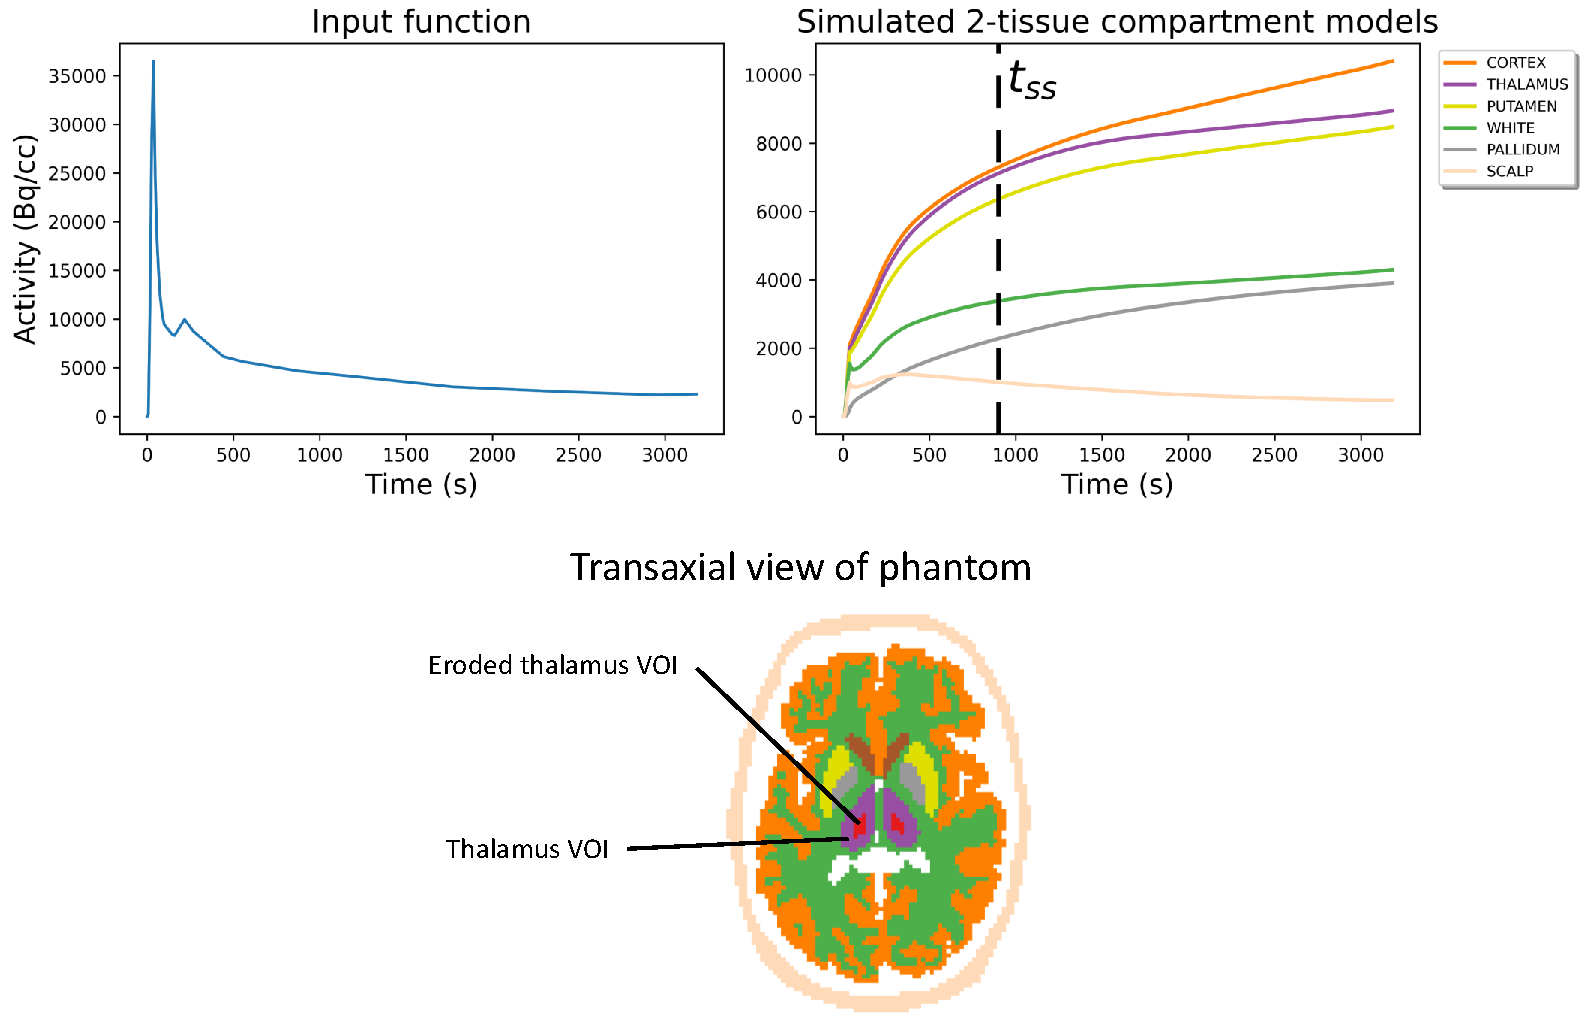
\includegraphics[width=140mm ,angle=0]{appendices/figures/phantom_TACs.pdf}
\caption{Input function and selection of simulated 2-tissue compartment model TACs (top), and transaxial view of the segmented zubal phantom, with the addition of an eroded thalamus VOI (bottom). The same colours are used for the TACs and the VOIs.} 
\label{fig:zubal_phantom}
\end{figure}


\begin{table}[ht!]
\centering
\caption{\label{tab:VOIs}VOIs used for evaluation.}
\begin{tabular}{llll}
\toprule
\textbf{VOI Name} & \textbf{Number of voxels} & \textbf{Volume ($cm^3$)}  \\
\midrule
Thalamus        & 915   & 12.40      \\
Eroded thalamus & 218   & 2.95       \\
Cortex          & 46588 & 631.36     \\
\toprule
\end{tabular}
\end{table}



    \chapter{Direct multi-bed dynamic reconstruction: Supplementary material}
\label{chap:AppendixC}

Supplementary graphs, used in the analysis of the evaluated IsotoPK studies of chapter~\ref{Chap3_3:IsotoPK}, are provided here. Additionally, an brief simulation study for the behaviour of the spectral analysis model in the liver and the effects from the dual-input function is included.

\section*{Supplementary graphs}

\begin{figure} [ht!]
\centering
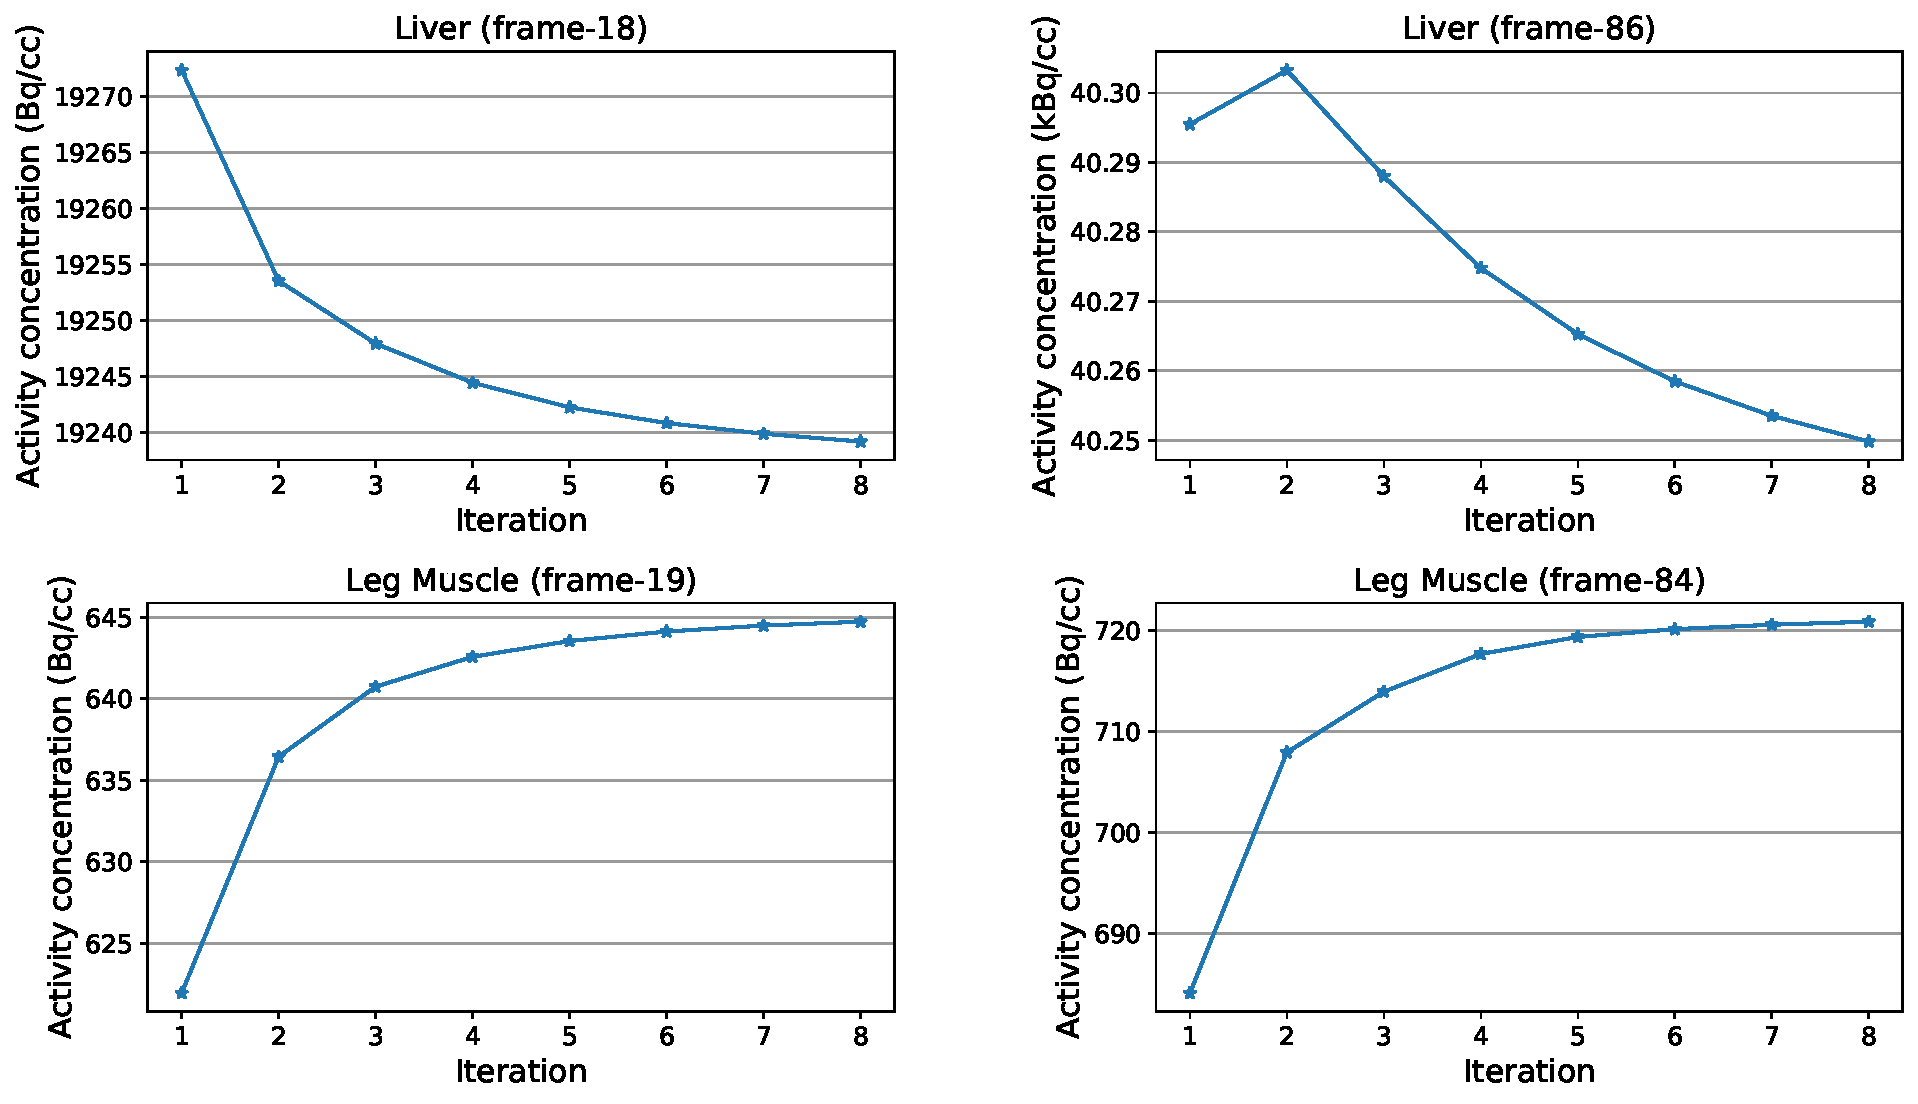
\includegraphics[scale=0.5,angle=0]{3_Results/3_3_DWB_Reconstruction/figures/3_3_IsotoPK_CTRL_DWB_3D_Convergence.pdf}
\caption{Liver (top) and Muscle (bottom) VOI mean versus iteration curves for 3D reconstruction. Shown for early (left) and late (right) frames of the \textit{CTRL} DWB acquisition including the DSB phase.}
\label{fig_3_3:IsotoPK_CTRL_DWB_4D_Convergence}
\end{figure} 

\begin{figure} [ht!]
\centering
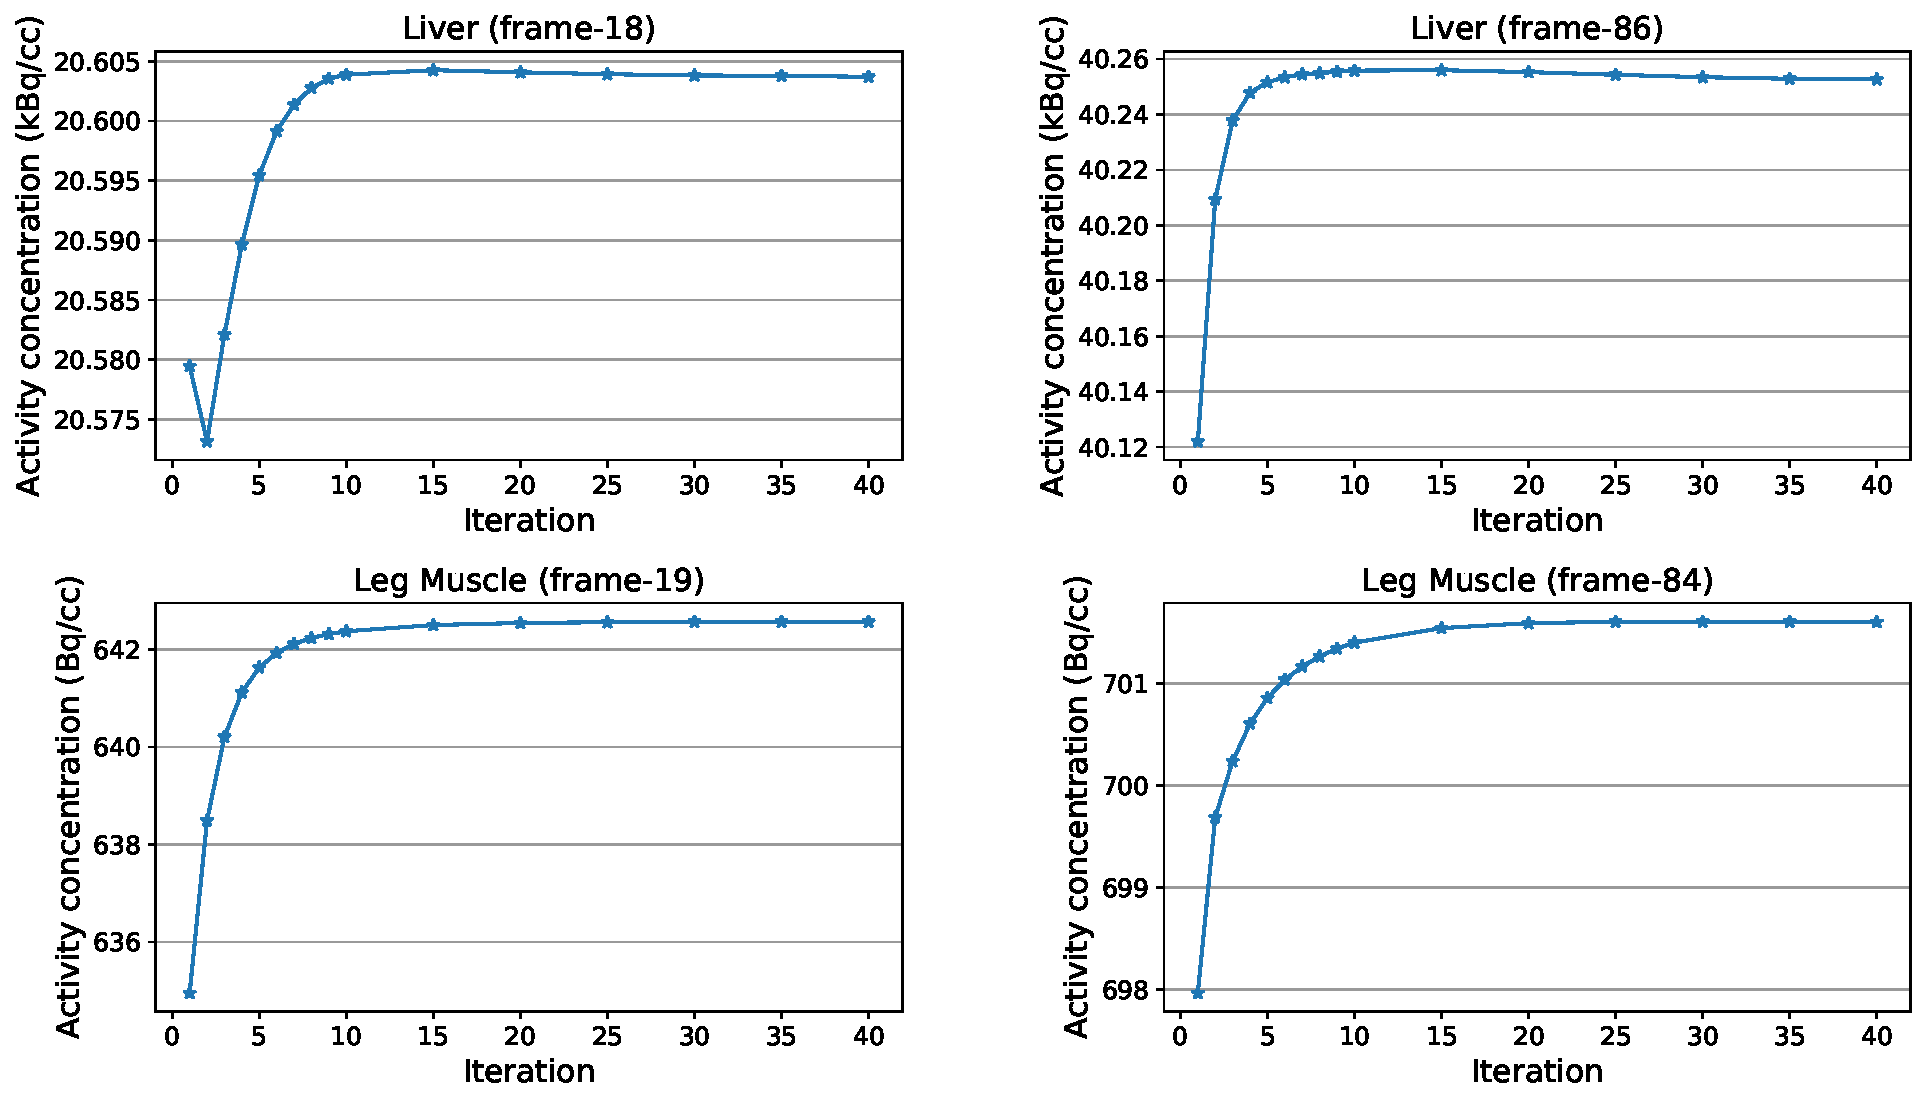
\includegraphics[scale=0.5,angle=0]{3_Results/3_3_DWB_Reconstruction/figures/3_3_IsotoPK_CTRL_DWB_4D_Convergence.pdf}
\caption{Liver (top) and Muscle (bottom) VOI mean versus iteration curves for 4D spectral reconstruction. Shown for early (left) and late (right) frames of the \textit{CTRL} DWB acquisition including the DSB phase.}
\label{fig_3_3:IsotoPK_CTRL_DSB_3D_Convergence}
\end{figure} 


\begin{figure} [ht!]
\centering
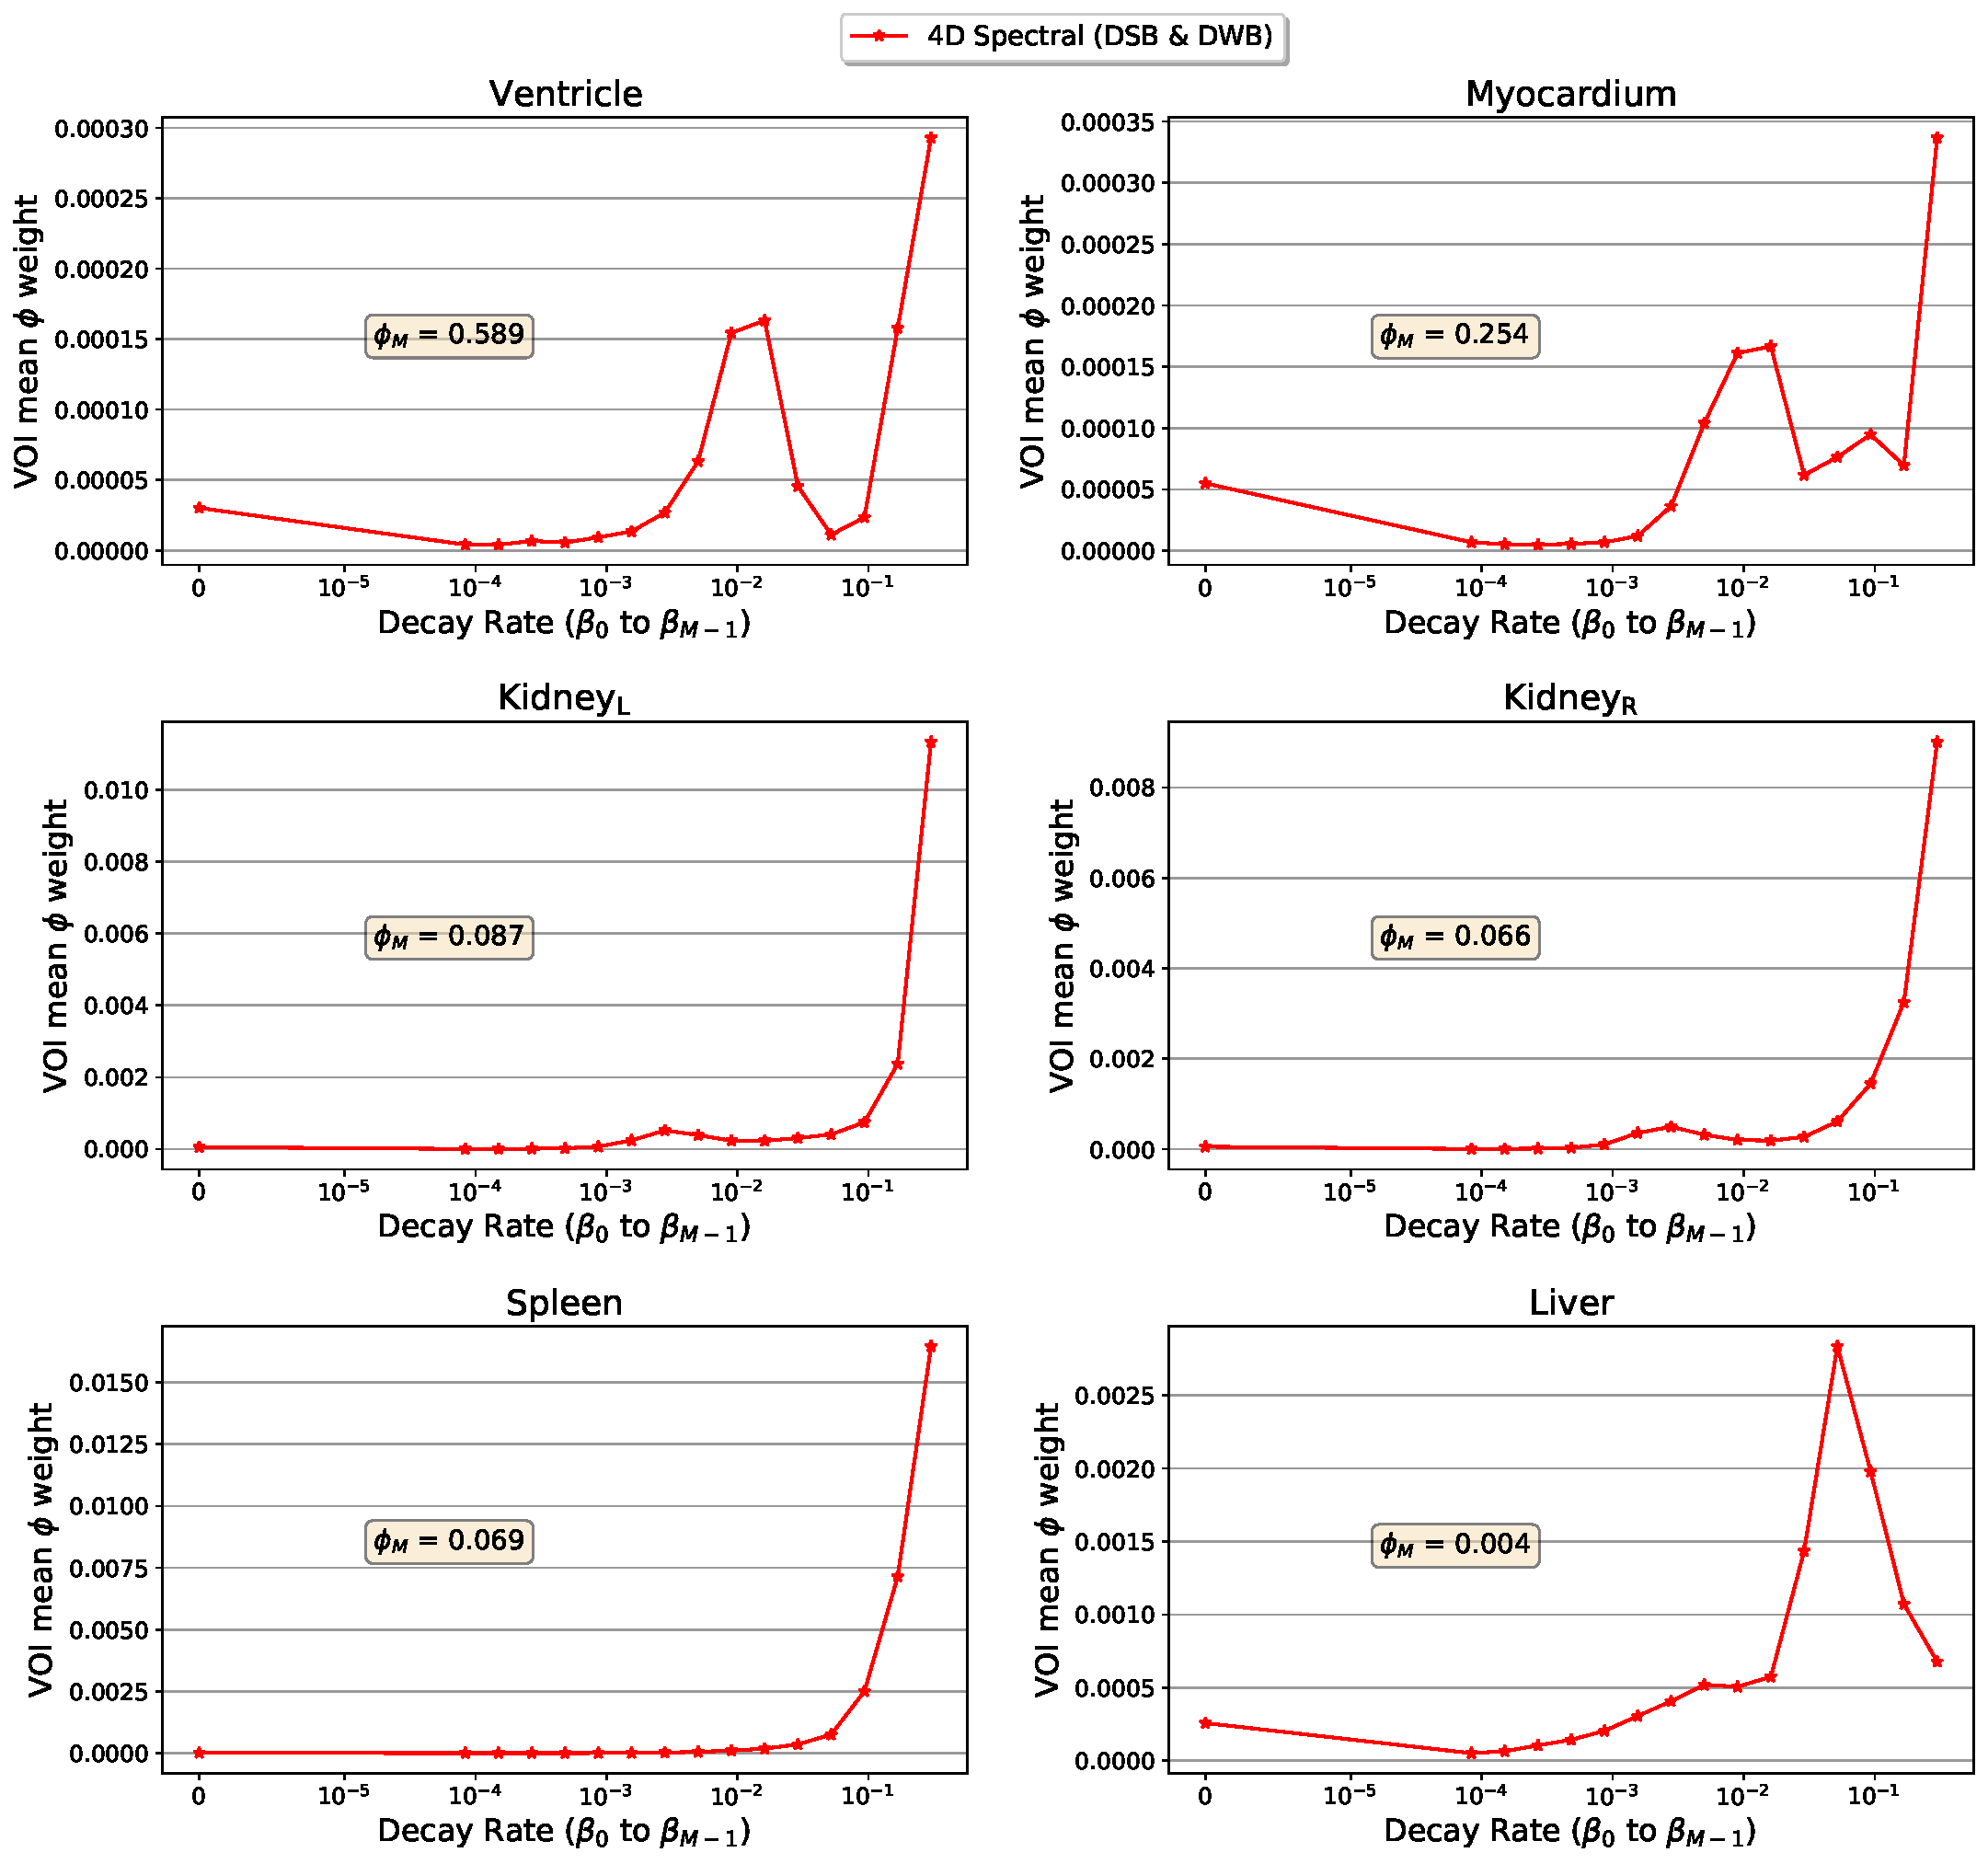
\includegraphics[scale=0.48,angle=0]{3_Results/3_3_DWB_Reconstruction/figures/3_3_IsotoPK_CTRL_DWB_SpectralParams_central_.pdf}
\caption{Spectral model coefficients average in VOIs. VOI regions shown which are included in both DSB and DWB acquisition.}
\label{fig_3_3:IsotoPK_CTRL_DWB_Spectrals}
\end{figure} 

\begin{figure} [ht!]
\centering
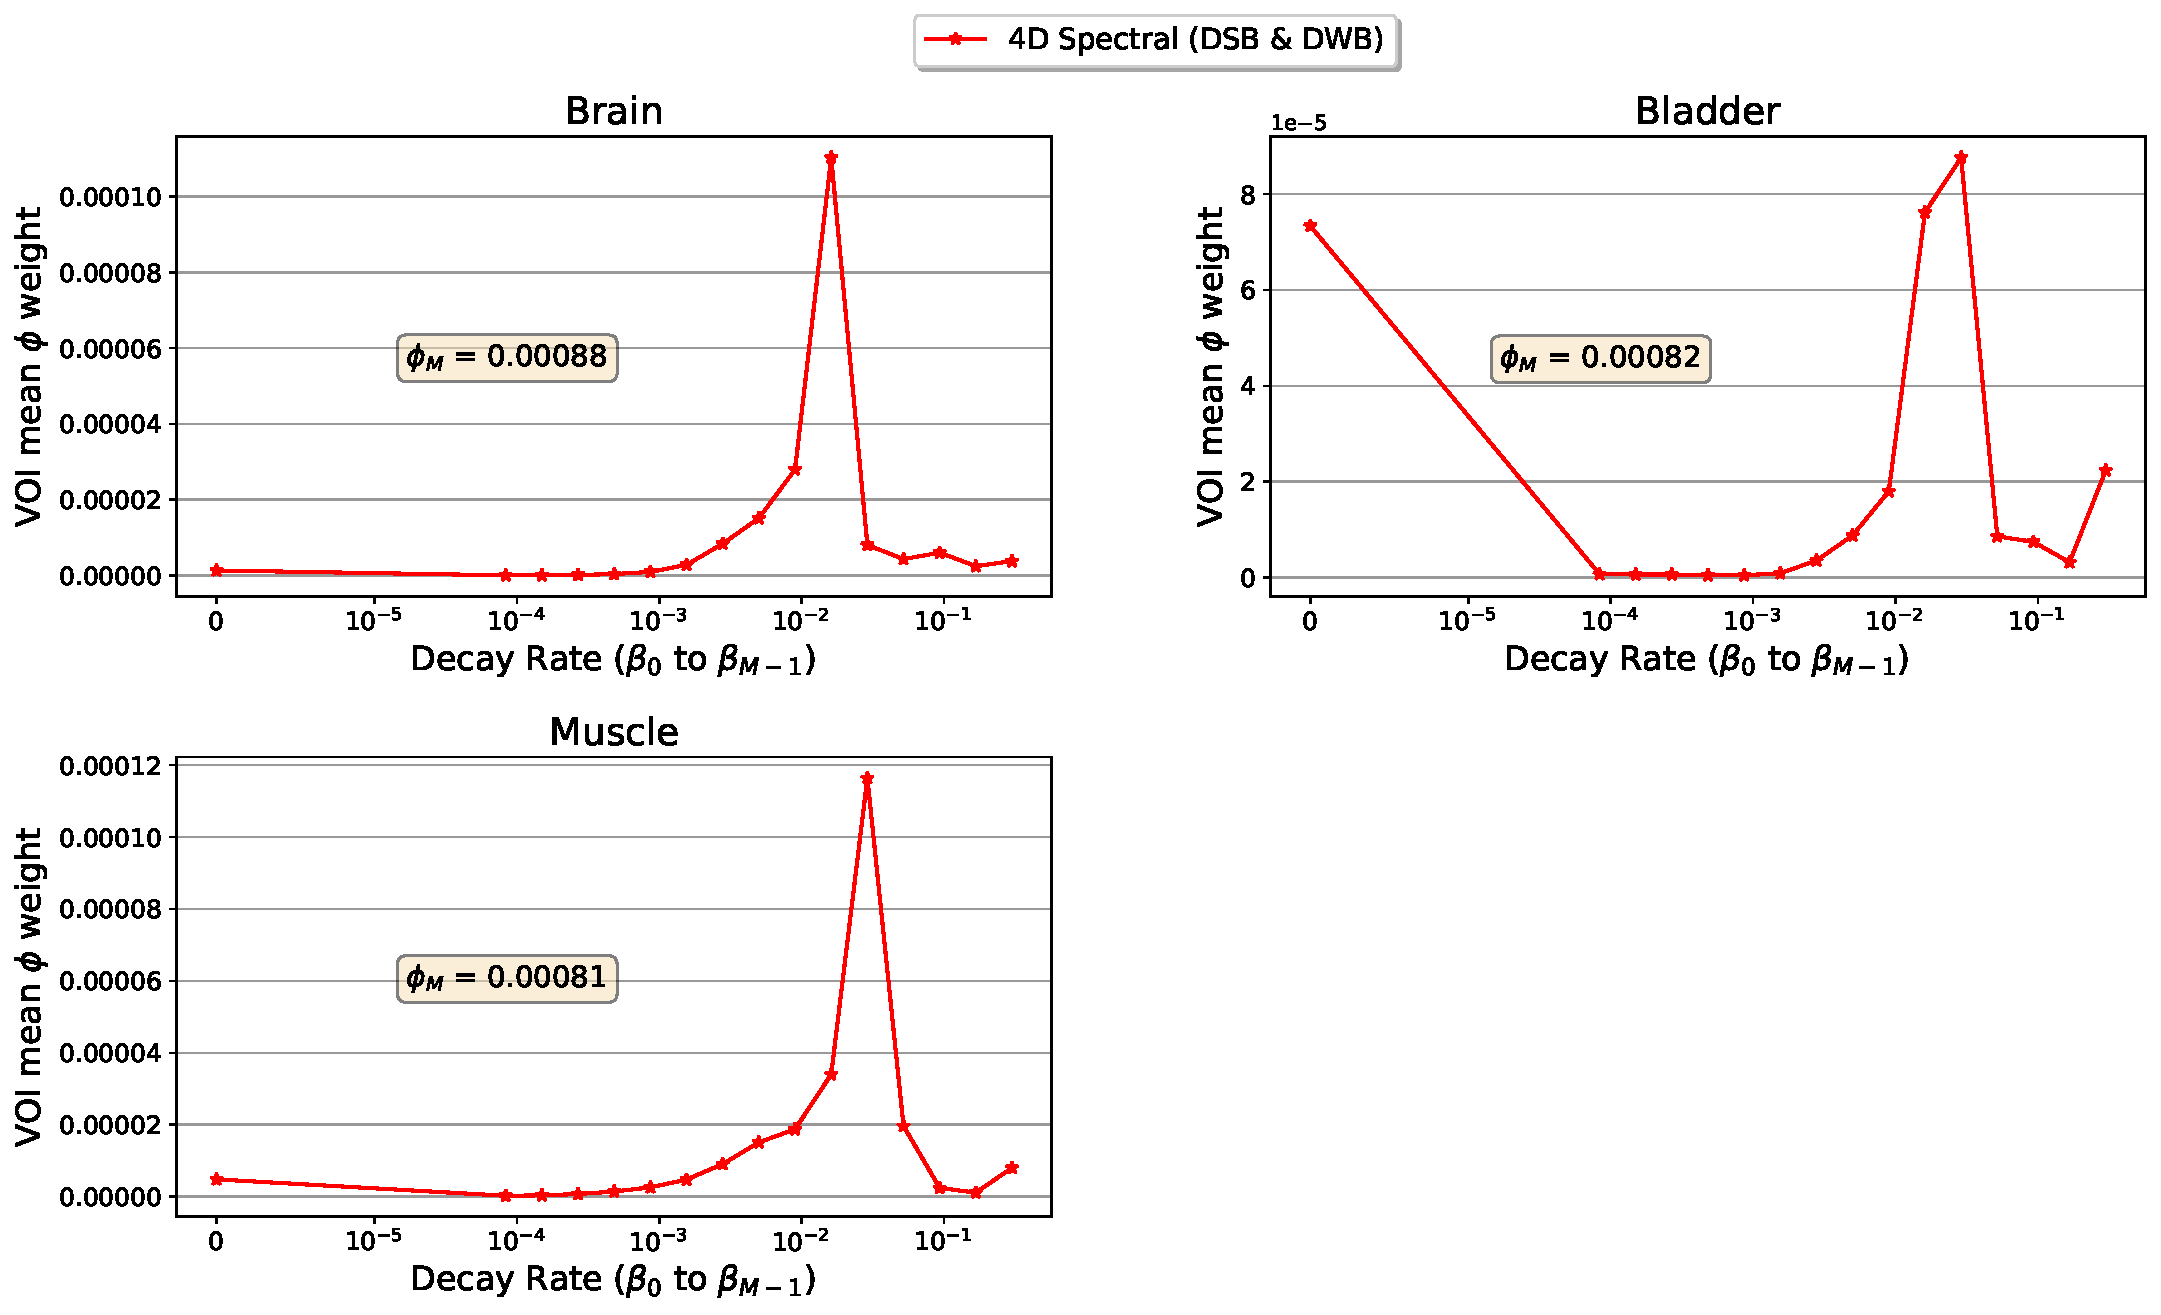
\includegraphics[scale=0.48,angle=0]{3_Results/3_3_DWB_Reconstruction/figures/3_3_IsotoPK_CTRL_DWB_SpectralParams_peripheral_.pdf}
\caption{Spectral model coefficients average in VOIs. VOI regions shown which are covered only by the DWB acquisition.}
\label{fig_3_3:IsotoPK_CTRL_DSB_Spectrals}
\end{figure} 

\clearpage
\section*{Liver dual-input function simulation study}
This short simulation was conducted using noiseless TACs to test the effects of the use of a dual input function model against spectral analysis that only accounts for one single input function.  
The following equations were used for the simulation. The portal vein input function was simulated using equation~\ref{eqn:Appendix_PortalVein} and a dispersion value $k_g=0.5 \mathrm{min}^{-1}$ from the literature~\cite{Kudomi2008}.
The dual input function was then simulated with a 25/75 ratio using equation~\ref{eqn:Appendix_HepaticInput} and provided to the equation~\ref{eqn:Appendix_2TCM} of the 2TC model for simulating liver TACs. Finally the blood fraction was included using equation~\ref{eqn:Appendix_CPET}. The simulated $K_1$ values varied between 0.3 and 2.4 min$^{-1}$. The simulated $k_2$, $k_3$ and $V_B$ values were 0.15 min$^{-1}$, 0.05 min$^{-1}$ and 0.03 respectively. These values, using a $K_1$= 0.7 min$^{-1}$, approach the TAC of the IsotoPK CTRL scan from chapter~\ref{Chap3_3:IsotoPK}. 
Spectral analysis was performed using the single input function of $C_{P}(t)$. 
%
\begin{equation} 
{C_{PV}}(t)  = {k_g} e^{-k_g t} \ast C_P(t)   \\ . \\
\label{eqn:Appendix_PortalVein}
\end{equation}
%
\begin{equation} 
{C_{H}}(t)  = 0.75 \cdot C_{PV}(t) + 0.25 \cdot C_{P}(t)  \\ . \\
\label{eqn:Appendix_HepaticInput}
\end{equation}
%
\begin{equation}
C_T(t) = K_1 ( e^{-(k_2+k_3)t} + \frac{k_3}{k_2+k_3}(1-e^{-(k_2+k_3)t})) \ast C_{H}(t)   
\label{eqn:Appendix_2TCM}
\end{equation}
%
\begin{equation}
{C_{PET}}(t)  = (1-V_{B}){C_{T}}(t) + V_{B}C_{H}(t) \\ , \\
\label{eqn:Appendix_CPET}
\end{equation}
%
%
The simulated TACs are shown in figure~\ref{fig_3_3:K1_Sims}, while the result $K_1^{*}$ values of the spectral analysis against simulated $K_1$ values are shown in~\ref{fig_3_3:K1_Sims_Results}. The results show an closely linear relationship between simulated $K_1$ and estimate $K_1^{*}$ values, with a deviation from a slope of 1. A part of this deviation is attributed to not correcting the $K_1^{*}$ values for blood fraction, but mostly it is due to unaccounted behaviour of the dual input function.
%
\begin{figure}[ht!]
\centering
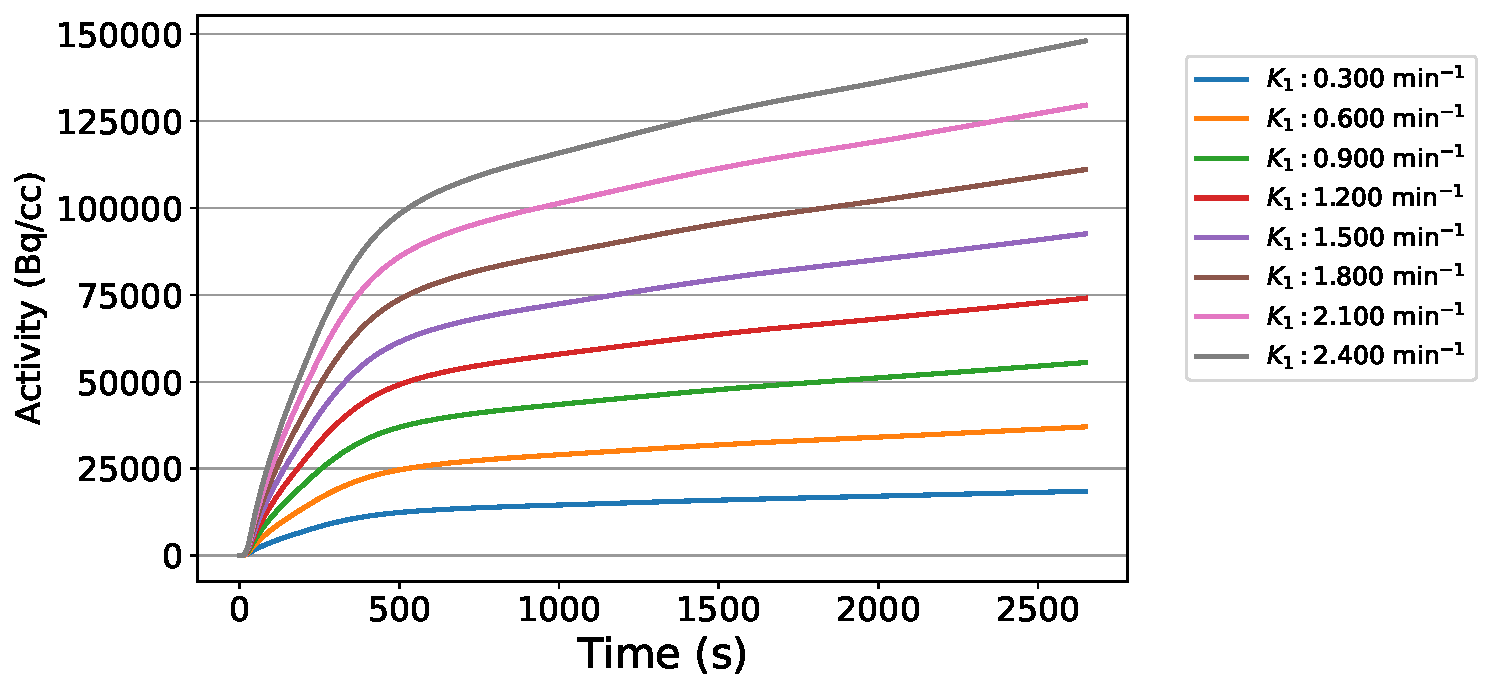
\includegraphics[scale=0.48,angle=0]{appendices/figures/ApendixC_multiple_K1.pdf}
\caption{Simulation of Liver TACs, using dual input function model and varying $K_1$ values.}
\label{fig_3_3:K1_Sims}
\end{figure} 
%
\begin{figure}[ht!]
\centering
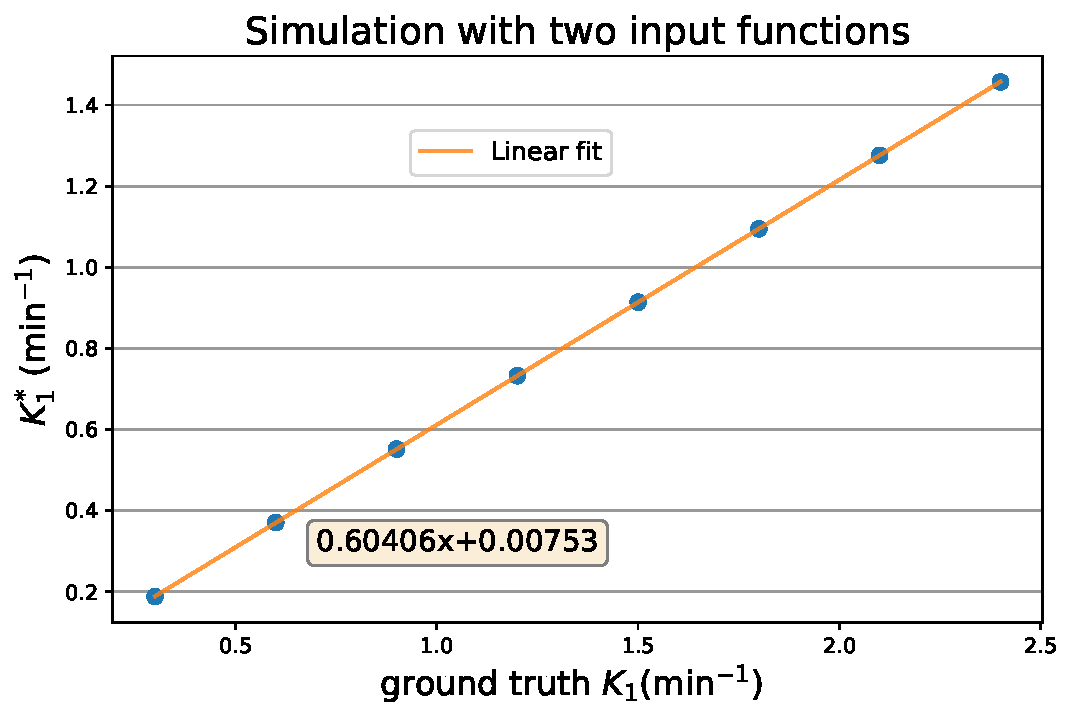
\includegraphics[scale=0.48,angle=0]{appendices/figures/ApendixC_multiple_K1_solution.pdf}
\caption{Result estimates of $K_1^{*}$ from spectral analysis on noiseless simulations of Liver TACs against ground truth simulated value.}
\label{fig_3_3:K1_Sims_Results}
\end{figure} 
    \end{appendices}
    

    \pagebreak
    \chapter*{Secondary Contributions}
\addcontentsline{toc}{chapter}{Secondary Contributions}
\label{Secondary_Contributions}

\textbf{PET FDG Improved Tumour Definition using Deep Learning}

Within the \gls{hybrid} secondments schedule, a 1-month secondment for Laura Dal Toso (LDT) from King's College London (KCL) was planned to take place at our lab. This secondment aimed in performing simulations for creation of large datasets that could be used for the training of Deep Learning (DL) methods.

For applications of PET imaging in oncology, quantification and shape of tumours are regularly used by medical professionals for the characterisation and classification of disease. For the case of \gls{nsclc} imaging, and not only limited to that, these image characteristics are often degraded by image noise and partial volume effects.
In this work, a method for improving tumour shape definition and quantification was proposed, by use of Deep Learning (DL). As DL methods require a large number of training datasets, simulations were used to train the proposed DL method. 

The aim was to ultimately use the DL method for real \gls{nsclc} image data from an mMR PET/MR scanner (installed at KCL). Thus the implementation of the mMR geometry in the PET analytical simulator was needed, which was performed by me (ZC) with guidance from Dr Simon Stute. After the successful integration of the geometry for simulations and validation of reconstructions using CASToR, a large dataset of ground truth tumours (placed within the XCAT phantom) was created by LDT and provided for PET simulation. A total of 2210 cases were simulated and reconstructed, using a custom made pipeline by ZC on two computer clusters of our lab.
Details on the methodology used and results will soon be submitted for publication as a research paper.

\textbf{Data Driven Motion Correction for Brain PET Dynamic Imaging}

A 2-week secondment was planned for me at the MUW in Vienna, with the aim of making use of dynamic reconstruction techniques developed during this PhD project to a cohort of epilepsy dynamic PET data. But this secondment was performed mostly from distance due to the pandemic and the time was spent towards the implementation and evaluation of novel motion estimation method for dynamic PET brain studies. 

Towards this goal, a method was developed using ultra-short frame reconstruction 
and a Cycle Generative Adversarial Network (cGAN). The cGAN was designed to improve image quality of the short frame reconstructions for better motion estimation. In the training of the cGAN, data from the cohort of epilepsy patients was used. The datasets had been acquired on an mMR PET/MR scanner.

During this project, a converter was adapted to support conversion of dynamic mMR PET data, including all corrections generated by the e7 tools, to the CASToR datafile format. Using the converted data, dynamic reconstructions were performed in CASToR using the involuntary motion correction option. These reconstructions were used to assess the effect of intra-frame motion correction in result activity and parametric images.
The development work and application of the cGAN has resulted in the publication of Shiyam Sundar \textit{et al.}~\cite{ShiyamSundar2020}. The work performed using CASToR has not been included in this publication, but it is considered for use in a future project on the topic of motion correction.

%\cleardoublepage
%\includepdf[pages=-]{SecondaryContributions/Formatted_Paper.pdf}
%\cleardoublepage
%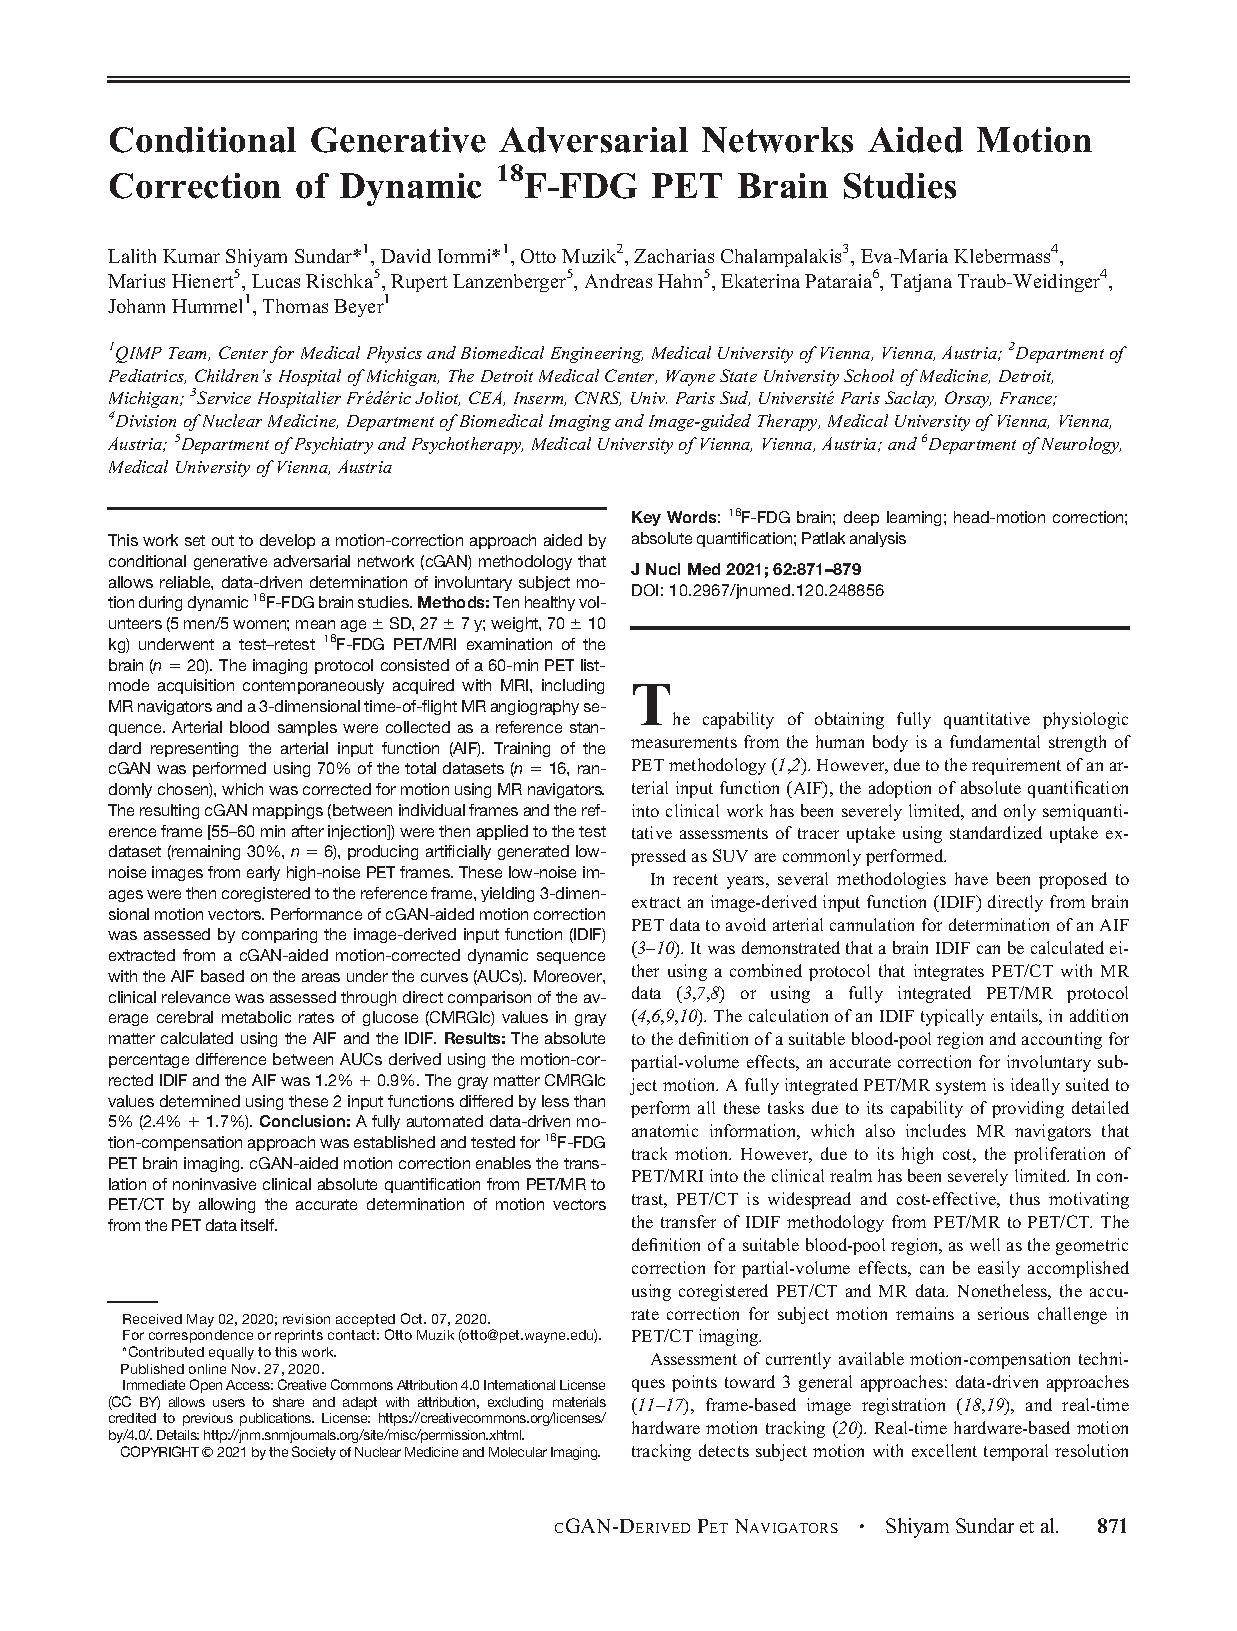
\includepdf[pages=-]{SecondaryContributions/871.full.pdf}
    \newpage 
    %%%%%%%%%%%%%%%%%%%%%%%%%%%%%%%%%%%%%%%%%%%%%%%%%%%%%%%%%%%%%%%%%%%%%%%%%%%%%%%%%%%%%%%%%%%%%%%%%%%%%%%%%%%%%%%%%%%%%%%%%%%%%%%%%%%%%%%%%%%%%%%%%%%%%%%%%%%%%%%%%%%%%%%
%%%%%%%%%%%%%%%%%%%%%%%%%%%%%%%%%%%%%%%%%%%%%%%%%%%%%%%%%%%%%%%%%%%%%%%%%%%%%%%%%%%%%%%%%%%%%%%%%%%%%%%%%%%%%%%%%%%%%%%%%%%%%%%%%%%%%%%%%%%%%%%%%%%%%%%%%%%%%%%%%%%%%%%
%%% Modèle pour la 4ème de couverture des thèses préparées à l'Université Paris-Saclay, basé sur le modèle produit par Nikolas STOTT / Template for back cover of thesis made at Université Paris-Saclay, based on the template made by Nikolas STOTT
%%% Mis à jour par Aurélien ARNOUX (École polytechnique)/ Updated by Aurélien ARNOUX (École polytechnique)
%%% Les instructions concernant chaque donnée à remplir sont données en bloc de commentaire / Rules to fill this file are given in comment blocks
%%% ATTENTION Ces informations doivent tenir sur une seule page une fois compilées / WARNING These informations must contain in no more than one page once compiled
%%%%%%%%%%%%%%%%%%%%%%%%%%%%%%%%%%%%%%%%%%%%%%%%%%%%%%%%%%%%%%%%%%%%%%%%%%%%%%%%%%%%%%%%%%%%%%%%%%%%%%%%%%%%%%%%%%%%%%%%%%%%%%%%%%%%%%%%%%%%%%%%%%%%%%%%%%%%%%%%%%%%%%%
%%% Version du 23 mai 2019 (Merci à Thibault CHEVALÉRIAS (CEA) pour ses suggestions et corrections)
%%%%%%%%%%%%%%%%%%%%%%%%%%%%%%%%%%%%%%%%%%%%%%%%%%%%%%%%%%%%%%%%%%%%%%%%%%%%%%%%%%%%%%%%%%%%%%%%%%%%%%%%%%%%%%%%%%%%%%%%%%%%%%%%%%%%%%%%%%%%%%%%%%%%%%%%%%%%%%%%%%%%%%%


\label{form_last}
%%%%%%%%%%%%%%%%%%%%%%%%%%%%%%%%%%%%%%%%%%%%%%%%%%%%%%%%%%%%%%%%%%%%%%%%%%%%%%%%%%%%%%%%%%%%%%%%%%%%%%%%%%%%%%%%%%%%%%%%%%%%%%%%%%%%%%%%%%%%%%%%%%%%%%%%%%%%%%%%%%%%%%%
%%%%%%%%%%%%%%%%%%%%%%%%%%%%%%%%%%%%%%%%%%%%%%%%%%%%%%%%%%%%%%%%%%%%%%%%%%%%%%%%%%%%%%%%%%%%%%%%%%%%%%%%%%%%%%%%%%%%%%%%%%%%%%%%%%%%%%%%%%%%%%%%%%%%%%%%%%%%%%%%%%%%%%%
%%% Formulaire / Form
%%% Remplacer les paramètres des \newcommand par les informations demandées / Replace \newcommand parameters by asked informations
%%%%%%%%%%%%%%%%%%%%%%%%%%%%%%%%%%%%%%%%%%%%%%%%%%%%%%%%%%%%%%%%%%%%%%%%%%%%%%%%%%%%%%%%%%%%%%%%%%%%%%%%%%%%%%%%%%%%%%%%%%%%%%%%%%%%%%%%%%%%%%%%%%%%%%%%%%%%%%%%%%%%%%%
%%%%%%%%%%%%%%%%%%%%%%%%%%%%%%%%%%%%%%%%%%%%%%%%%%%%%%%%%%%%%%%%%%%%%%%%%%%%%%%%%%%%%%%%%%%%%%%%%%%%%%%%%%%%%%%%%%%%%%%%%%%%%%%%%%%%%%%%%%%%%%%%%%%%%%%%%%%%%%%%%%%%%%%

\newcommand{\logoEd}{ed}																		%% Logo de l'école doctorale. Indiquer le sigle / Doctoral school logo. Indicate the acronym : 2MIB; AAIF; ABIES; BIOSIGNE; CBMS; EDMH; EDOM; EDPIF; EDSP; EOBE; INTERFACES; ITFA; PHENIICS; SDSV; SDV; SHS; SMEMAG; SSMMH; STIC
\newcommand{\PhDTitleFR}{titre (en français)}													%% Titre de la thèse en français / Thesis title in french
\newcommand{\keywordsFR}{3 à 6 mots clés}														%% Mots clés en français, séprarés par des , / Keywords in french, separated by ,
\newcommand{\abstractFR}{\lipsum[1-3]}															%% Résumé en français / abstract in french

\newcommand{\PhDTitleEN}{titre (en anglais)}													%% Titre de la thèse en anglais / Thesis title in english
\newcommand{\keywordsEN}{3 à 6 mots clés}														%% Mots clés en anglais, séprarés par des , / Keywords in english, separated by ,
\newcommand{\abstractEN}{\lipsum[1-3]}															%% Résumé en anglais / abstract in english

\label{layout_last}
%%%%%%%%%%%%%%%%%%%%%%%%%%%%%%%%%%%%%%%%%%%%%%%%%%%%%%%%%%%%%%%%%%%%%%%%%%%%%%%%%%%%%%%%%%%%%%%%%%%%%%%%%%%%%%%%%%%%%%%%%%%%%%%%%%%%%%%%%%%%%%%%%%%%%%%%%%%%%%%%%%%%%%%
%%%%%%%%%%%%%%%%%%%%%%%%%%%%%%%%%%%%%%%%%%%%%%%%%%%%%%%%%%%%%%%%%%%%%%%%%%%%%%%%%%%%%%%%%%%%%%%%%%%%%%%%%%%%%%%%%%%%%%%%%%%%%%%%%%%%%%%%%%%%%%%%%%%%%%%%%%%%%%%%%%%%%%%
%%% Mise en page / Page layout      
%%% NE RIEN MODIFIER / DO NOT MODIFY
%%%%%%%%%%%%%%%%%%%%%%%%%%%%%%%%%%%%%%%%%%%%%%%%%%%%%%%%%%%%%%%%%%%%%%%%%%%%%%%%%%%%%%%%%%%%%%%%%%%%%%%%%%%%%%%%%%%%%%%%%%%%%%%%%%%%%%%%%%%%%%%%%%%%%%%%%%%%%%%%%%%%%%%
%%%%%%%%%%%%%%%%%%%%%%%%%%%%%%%%%%%%%%%%%%%%%%%%%%%%%%%%%%%%%%%%%%%%%%%%%%%%%%%%%%%%%%%%%%%%%%%%%%%%%%%%%%%%%%%%%%%%%%%%%%%%%%%%%%%%%%%%%%%%%%%%%%%%%%%%%%%%%%%%%%%%%%%

\pagestyle{empty}

%%% Logo de l'école doctorale. Le nom du fichier correspond au sigle de l'ED / Doctoral school logo. Filename correspond to doctoral school acronym
%%% Les noms valides sont / Valid names are : 2MIB; AAIF; ABIES; BIOSIGNE; CBMS; EDMH; EDOM; EDPIF; EDSP; EOBE; INTERFACES; ITFA; PHENIICS; SDSV; SDV; SHS; SMEMAG; SSMMH; STIC
\begin{textblock*}{61mm}(16mm,3mm)
    \textblockcolour{white}
	\noindent\includegraphics[height=24mm]{media/ed/\logoEd.jpeg}
\end{textblock*}



%%%Titre de la thèse en français / Thesis title in french
\begin{singlespace}
\begin{center}
\fcolorbox{bordeau}{white}{\parbox{0.95\textwidth}{
{\bf Titre:} \PhDTitleFR 
\medskip

%%%Mots clés en français, séprarés par des ; / Keywords in french, separated by ;
{\bf Mots clés:} \keywordsFR 
\vspace{-2mm}

%%% Résumé en français / abstract in french
\begin{multicols}{2}
{\bf Résumé:} 
\abstractFR 
\end{multicols}
}}
\end{center}

\vspace*{0mm}

%%%Titre de la thèse en anglais / Thesis title in english
\begin{center}
\fcolorbox{bordeau}{white}{\parbox{0.95\textwidth}{
{\bf Title:} \PhDTitleEN 

\medskip

%%%Mots clés en anglais, séprarés par des ; / Keywords in english, separated by ;
{\bf Keywords:}  \keywordsEN %%3 à 6 mots clés%%
\vspace{-2mm}
\begin{multicols}{2}
	
%%% Résumé en anglais / abstract in english
{\bf Abstract:} 
\abstractEN
\end{multicols}
}}
\end{center}

\begin{textblock*}{161mm}(10mm,270mm)
\textblockcolour{white}
\color{bordeau}
{\bf\noindent Université Paris-Saclay	         }

\noindent Espace Technologique / Immeuble Discovery 

\noindent Route de l’Orme aux Merisiers RD 128 / 91190 Saint-Aubin, France 
\end{textblock*}

\begin{textblock*}{0mm}(182mm,255mm)
\textblockcolour{white}

\includegraphics[width=20mm]{media/UPSACLAY-petit}
\end{textblock*}
\end{singlespace}
\end{document}